\documentclass[UTF8, a4paper, 11pt]{article}
\usepackage{diagbox}
\usepackage{subfigure}
\usepackage[UTF8, scheme=plain]{ctex}
\usepackage{fontspec}
\usepackage{float}
\usepackage{amsmath}
\newtheorem{myDef}{Definition}
\usepackage{graphicx}
\usepackage{geometry}
\usepackage{listings}
\usepackage{xcolor}
\usepackage{caption}
\geometry{scale=0.8}
\linespread{1.5}
\usepackage{hyperref}
\usepackage{color}
\usepackage{fontspec}
\usepackage{enumitem}
\usepackage[linesnumbered,boxed]{algorithm2e}    
\usepackage{xeCJK}
\usepackage{indentfirst} 
\graphicspath{{Pics/}} 	% 在于.tex同级的目录下创建名为pic的文件夹,存放图片


\setlength{\parindent}{2em}

\lstset{
    language={C},
    frame=shadowbox,
    breaklines=true,
    numbers=left,
    backgroundcolor=\color[RGB]{245,245,244},
    rulesepcolor=\color{red!20!green!20!blue!20},
    numberstyle={\color[RGB]{0,192,192}\tiny},
    basicstyle=\footnotesize \fontspec{Source Code Pro}
}
\setenumerate[1]{itemsep=0pt,partopsep=0pt,parsep=\parskip,topsep=0pt}
\setitemize[1]{itemsep=0pt,partopsep=0pt,parsep=\parskip,topsep=0pt}
\setdescription{itemsep=0pt,partopsep=0pt,parsep=\parskip,topsep=0pt}


\title{	
\normalfont \normalsize
\textsc{School of Data and Computer Science, Sun Yat-sen University} \\ [25pt] %textsc small capital letters
\rule{\textwidth}{0.5pt} \\[0.4cm] % Thin top horizontal rule
\huge 数电实验2\\ % The assignment title
\rule{\textwidth}{2pt} \\[0.5cm] % Thick bottom horizontal rule
\author{18308045 谷正阳}
\date{\normalsize\today}
}

\begin{document}
\maketitle
\tableofcontents
\newpage
\section{仿真实验}
\subsection{ex2.1}
\subsubsection{电路图}
\begin{figure}[H]
    \centering
    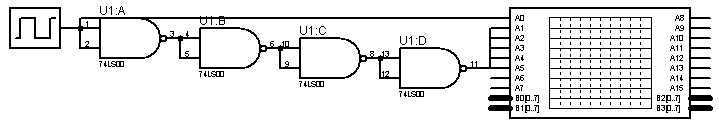
\includegraphics[width=0.8\textwidth]{ex2.1电路图.jpg}
\end{figure}
\subsubsection{波形图}
\begin{figure}[H]
    \centering
    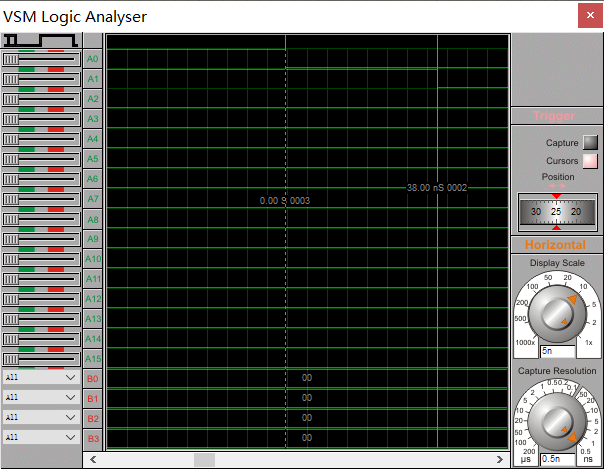
\includegraphics[width=0.8\textwidth]{ex2.1波形图.png}
\end{figure}
在把捕捉分辨率跳到很低的时候,可以看出$t_{pd}=\frac{38ns}4=9.5ns$。
\subsection{ex2.2}
\subsubsection{电路图}
\begin{figure}[H]
    \centering
    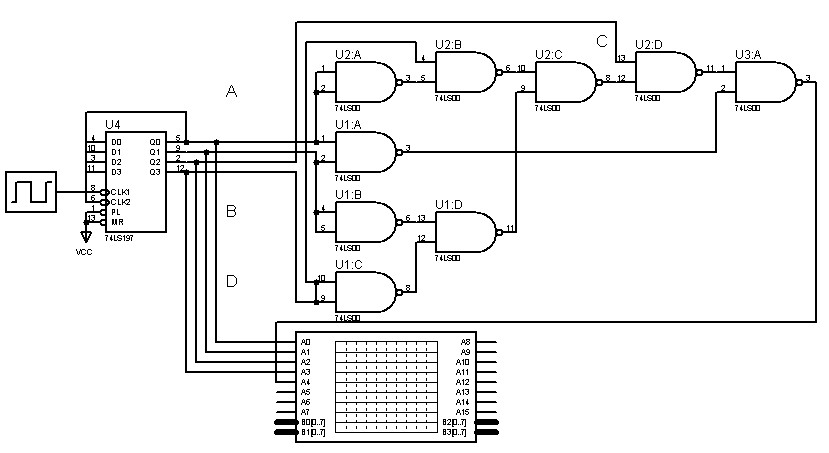
\includegraphics[width=0.8\textwidth]{ex2.2电路图.jpg}
\end{figure}
\subsubsection{真值表}
$$\begin{aligned}
F=&\overline{\overline{AB}\cdot\overline{C\cdot(\overline{\overline{\bar B\bar D}\cdot\overline{\bar AD}})}}\\
=&AB+C\cdot(\overline{\overline{\bar B\bar D}\cdot\overline{\bar AD}})\\
=&AB+C\cdot(\bar B\bar D+\bar AD)\\
=&AB+\bar BC\bar D+\bar ACD
\end{aligned}$$
\begin{table}[H]
\center
\begin{tabular}{|l|l|l|l|l|}
\hline
$A$ & $B$ & $C$ & $D$ & $F$ \\ \hline
0   & 0   & 0   & 0   & 0   \\ \hline
1   & 0   & 0   & 0   & 0   \\ \hline
0   & 1   & 0   & 0   & 0   \\ \hline
1   & 1   & 0   & 0   & 1   \\ \hline
0   & 0   & 1   & 0   & 1   \\ \hline
1   & 0   & 1   & 0   & 1   \\ \hline
0   & 1   & 1   & 0   & 0   \\ \hline
1   & 1   & 1   & 0   & 1   \\ \hline
0   & 0   & 0   & 1   & 0   \\ \hline
1   & 0   & 0   & 1   & 0   \\ \hline
0   & 1   & 0   & 1   & 0   \\ \hline
1   & 1   & 0   & 1   & 1   \\ \hline
0   & 0   & 1   & 1   & 1   \\ \hline
1   & 0   & 1   & 1   & 0   \\ \hline
0   & 1   & 1   & 1   & 1   \\ \hline
1   & 1   & 1   & 1   & 1   \\ \hline  
\end{tabular}
\end{table}
\subsubsection{波形图}
\begin{figure}[H]
    \centering
    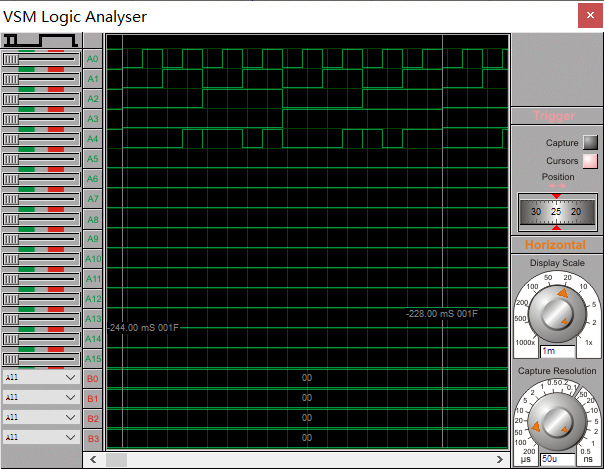
\includegraphics[width=0.8\textwidth]{ex2.2波形图.png}
\end{figure}
A0,A1,A2,A3分别算A,B,C,D,可以看出和真值表一样,但是有几处毛刺。
\subsection{ex2.3}
\subsubsection{卡诺图}
\begin{table}[H]
\center
\begin{tabular}{|l|l|l|l|l|}
\hline
\diagbox{AB}{CD} & 00 & 01 & 11 & 10 \\ \hline
00               &    &    & 1  & 1  \\ \hline
01               &    &    & 1  &    \\ \hline
11               & 1  & 1  & 1  & 1  \\ \hline
10               &    &    &    & 1  \\ \hline
\end{tabular}
\end{table}
\subsubsection{冗余}
$$\begin{aligned}
F=&AB+\bar BC\bar D+\bar ACD\\
=&AB+\bar BC\bar D+\bar ACD+BCD+AC\bar D+\bar A\bar BC\\
=&\overline{\overline{AB}\cdot\overline{C\cdot(\overline{\overline{\bar B\bar D}\cdot\overline{\bar AD}})}}+BCD+AC\bar D+\bar A\bar BC\\
\end{aligned}$$
在此只解决$A$的毛刺,因而只加$BCD$一项。
\subsubsection{电路图}
\begin{figure}[H]
    \centering
    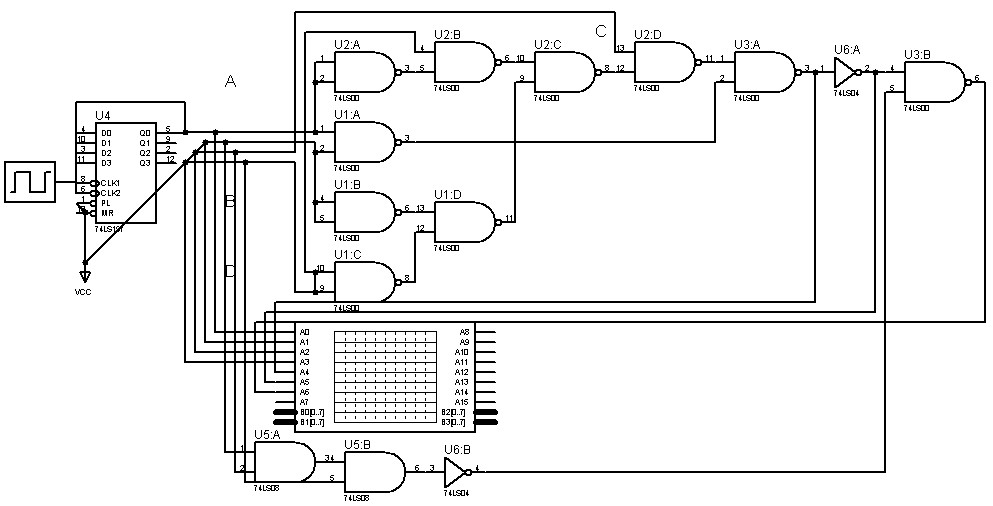
\includegraphics[width=0.8\textwidth]{ex2.3电路图.jpg}
\end{figure}
\subsubsection{波形图}
\begin{figure}[H]
    \centering
    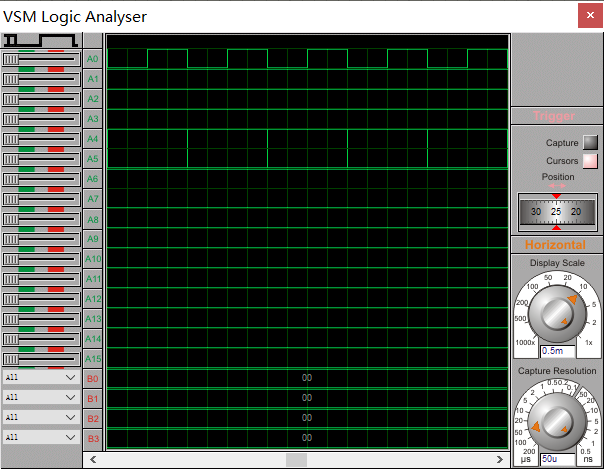
\includegraphics[width=0.8\textwidth]{ex2.3波形图.png}
\end{figure}
A0,A1,A2,A3分别是A,B,C,D,A4是F有毛刺,A5是F加反相器仍有毛刺,A6是F加冗余解决毛刺。
\subsection{ex2.4}
\subsubsection{电路图}
\begin{figure}[H]
    \centering
    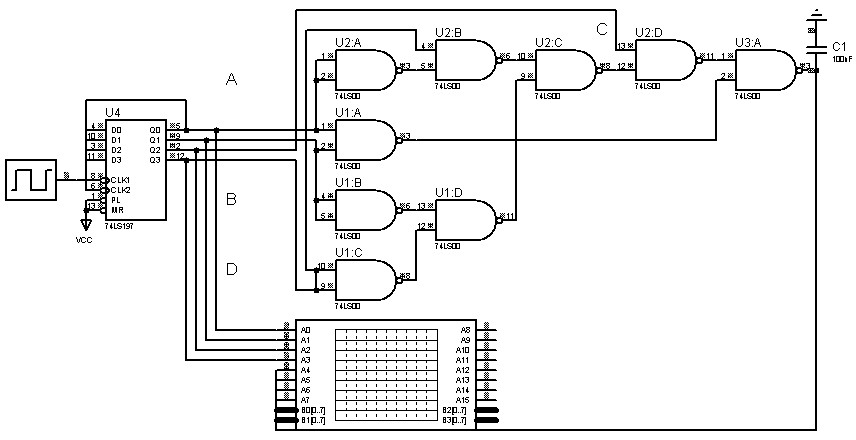
\includegraphics[width=0.8\textwidth]{ex2.4电路图.jpg}
\end{figure}
\subsubsection{波形图}
\begin{figure}[H]
    \centering
    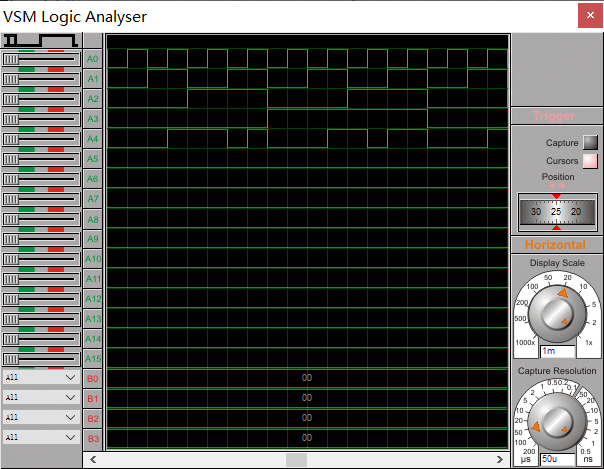
\includegraphics[width=0.8\textwidth]{ex2.4波形图.png}
\end{figure}
发现并联电容可以解决毛刺。
\section{实验箱实验}
\subsection{五、1.}
\begin{figure}[H]
    \centering
    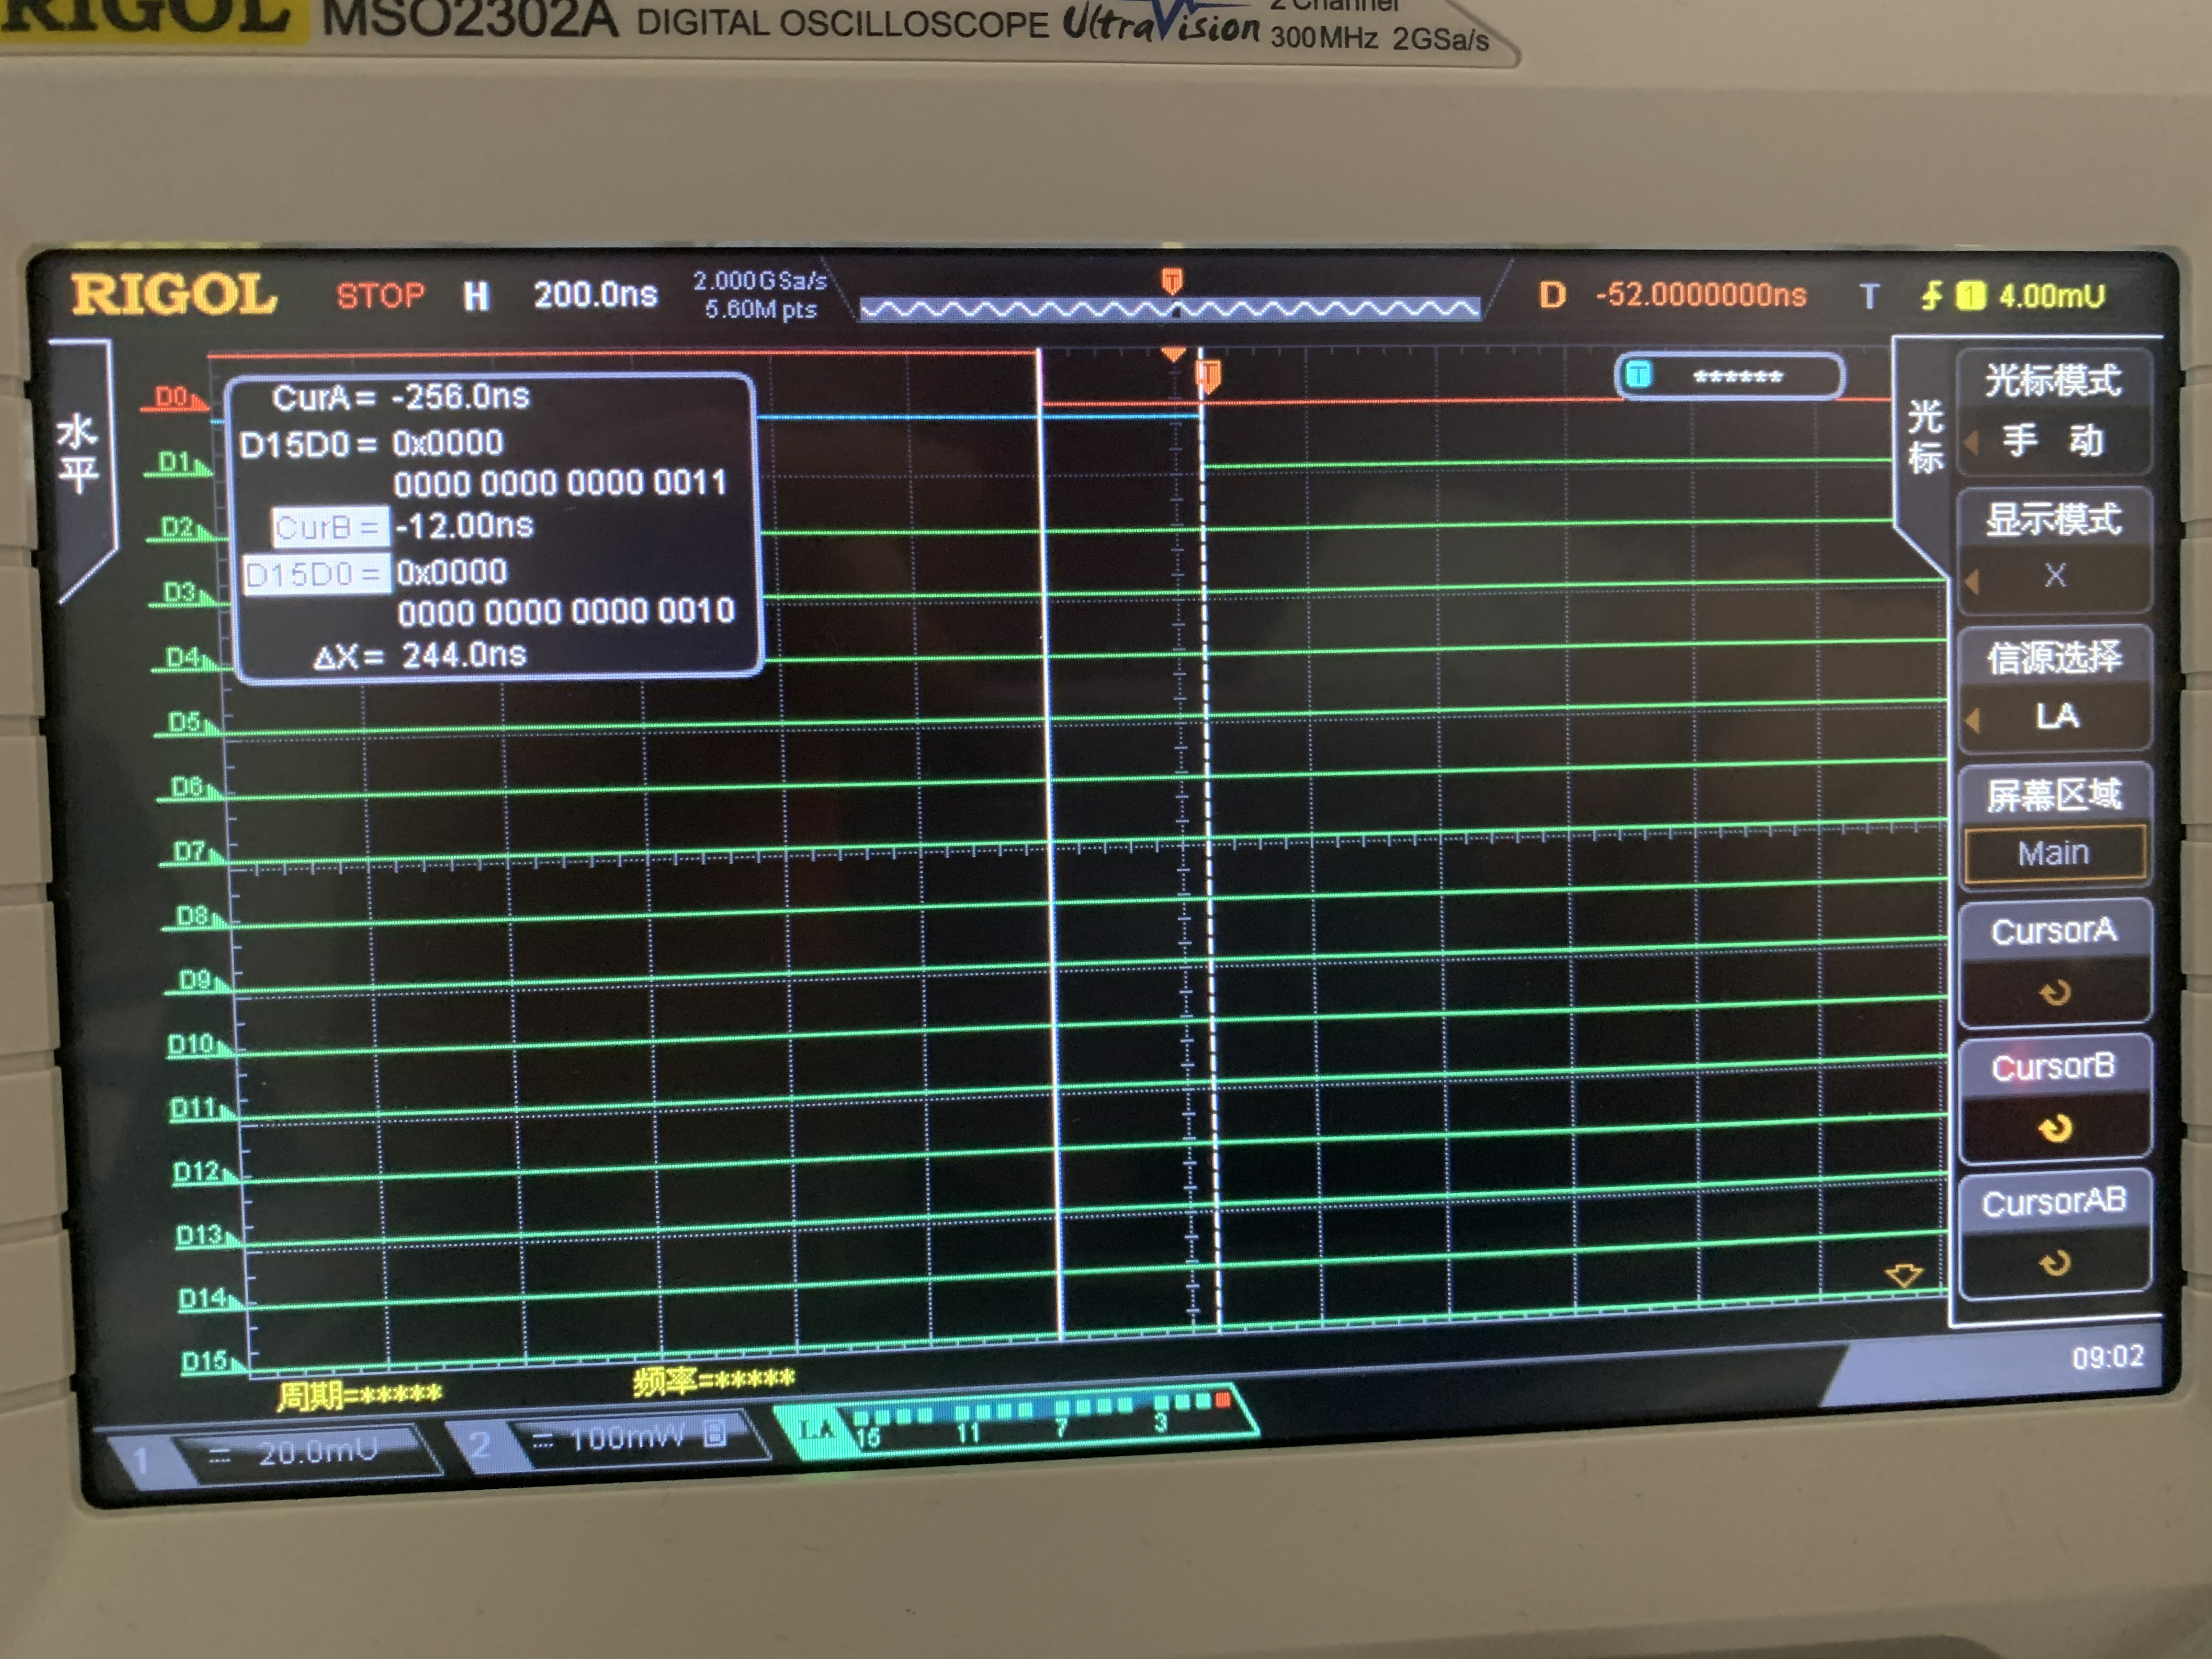
\includegraphics[width=0.8\textwidth]{延迟.JPG}
\end{figure}
$$t_{pd}=\frac{-12ns-(-256ns)}{4}=61ns$$
\subsection{五、2.}
\subsubsection{五、2.(3)}
下面以D、C、B、A按4位二进制数递增来排列:
\begin{figure}[H]
    \centering
    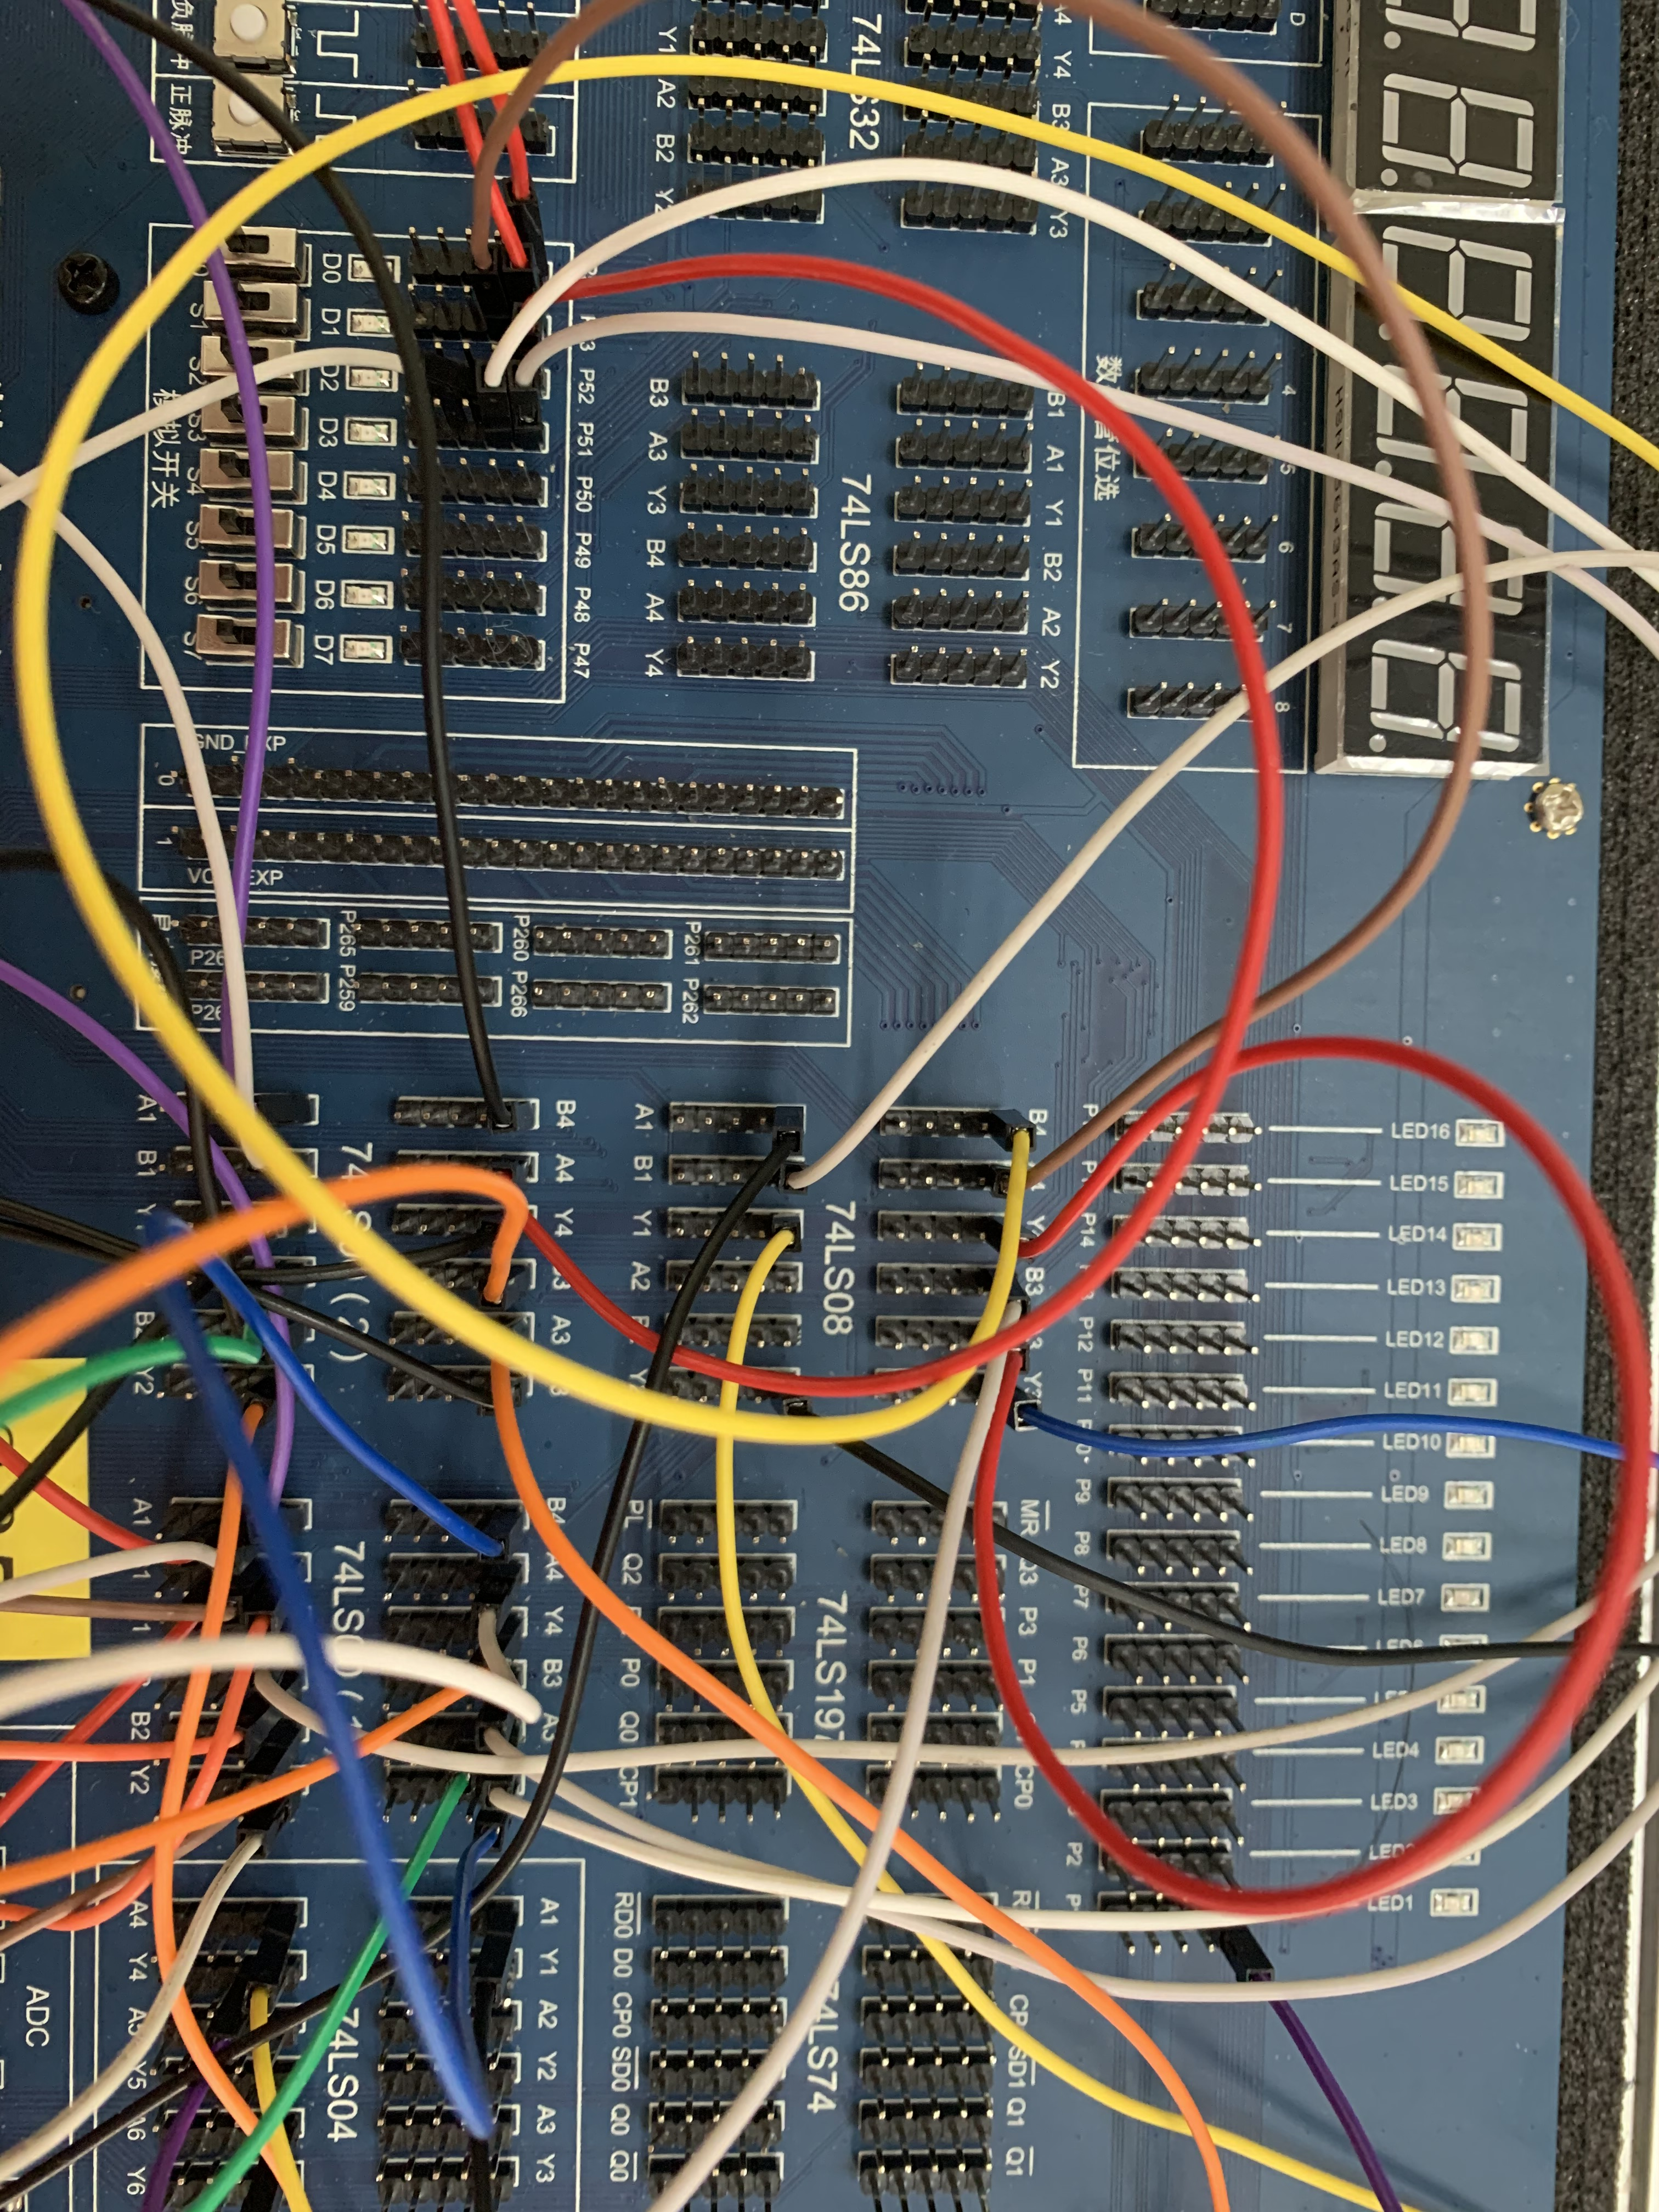
\includegraphics[width=0.8\textwidth]{0000.JPG}
\end{figure}
\begin{figure}[H]
    \centering
    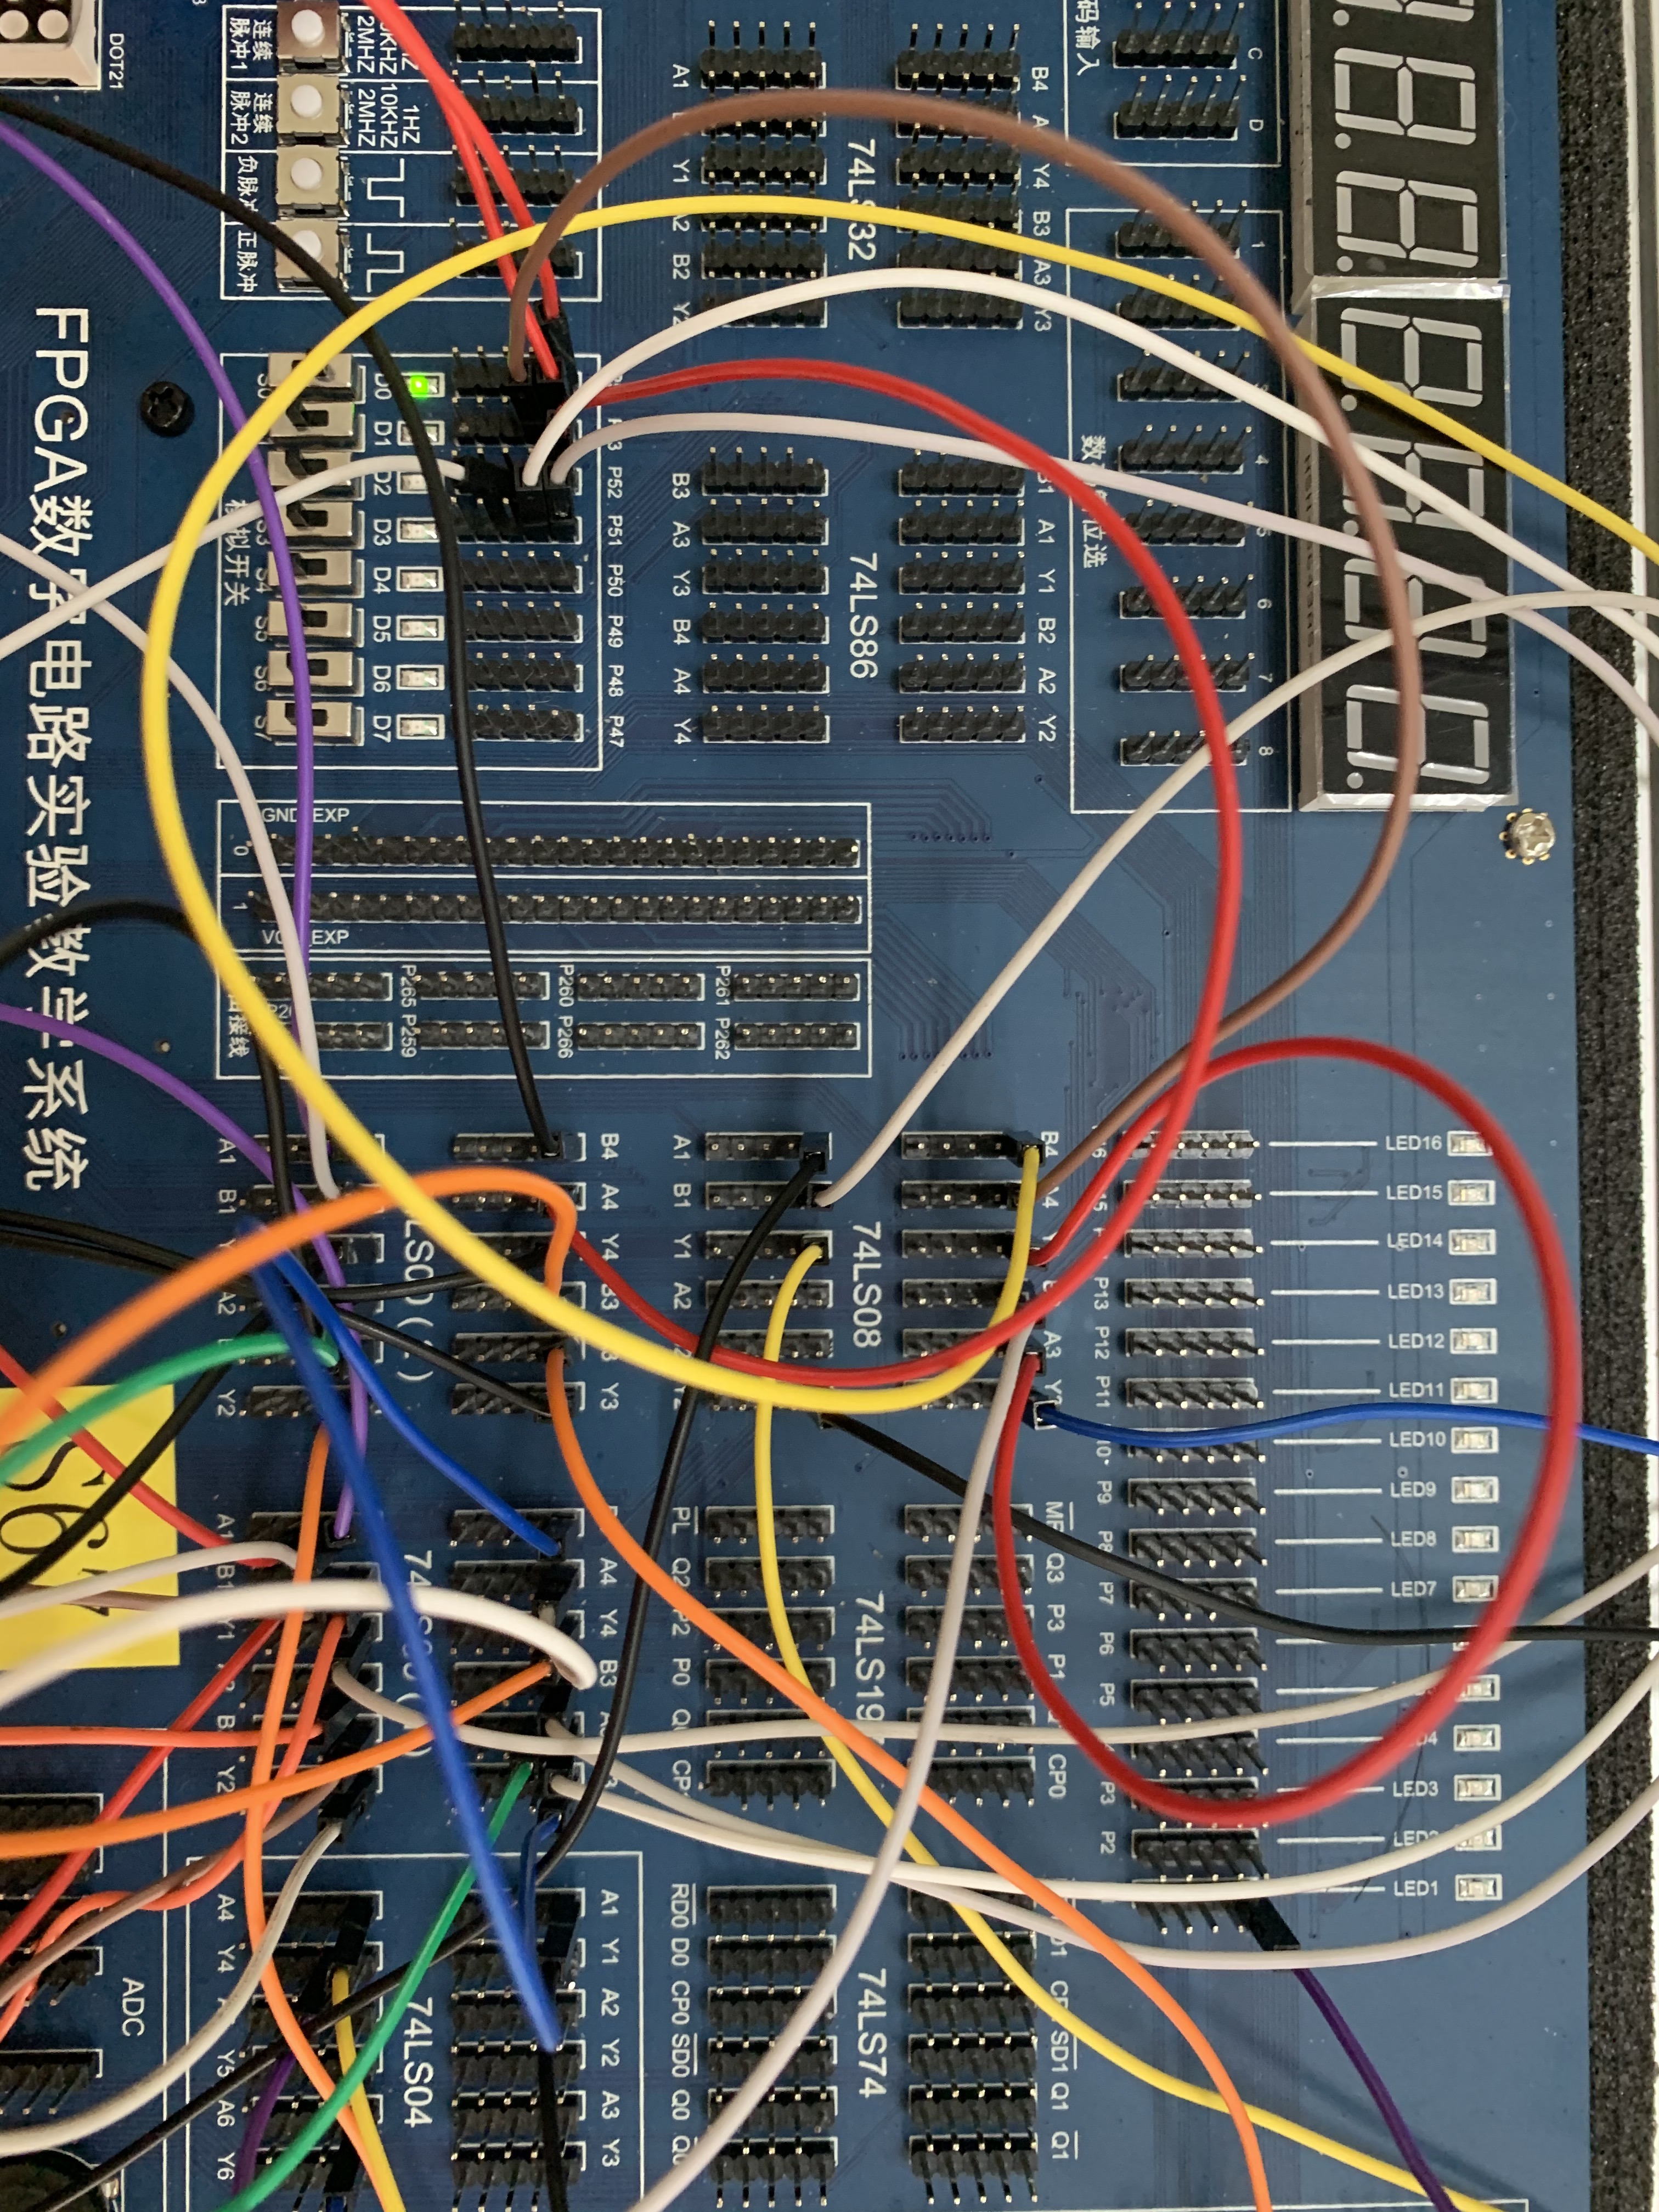
\includegraphics[width=0.8\textwidth]{0001.JPG}
\end{figure}
\begin{figure}[H]
    \centering
    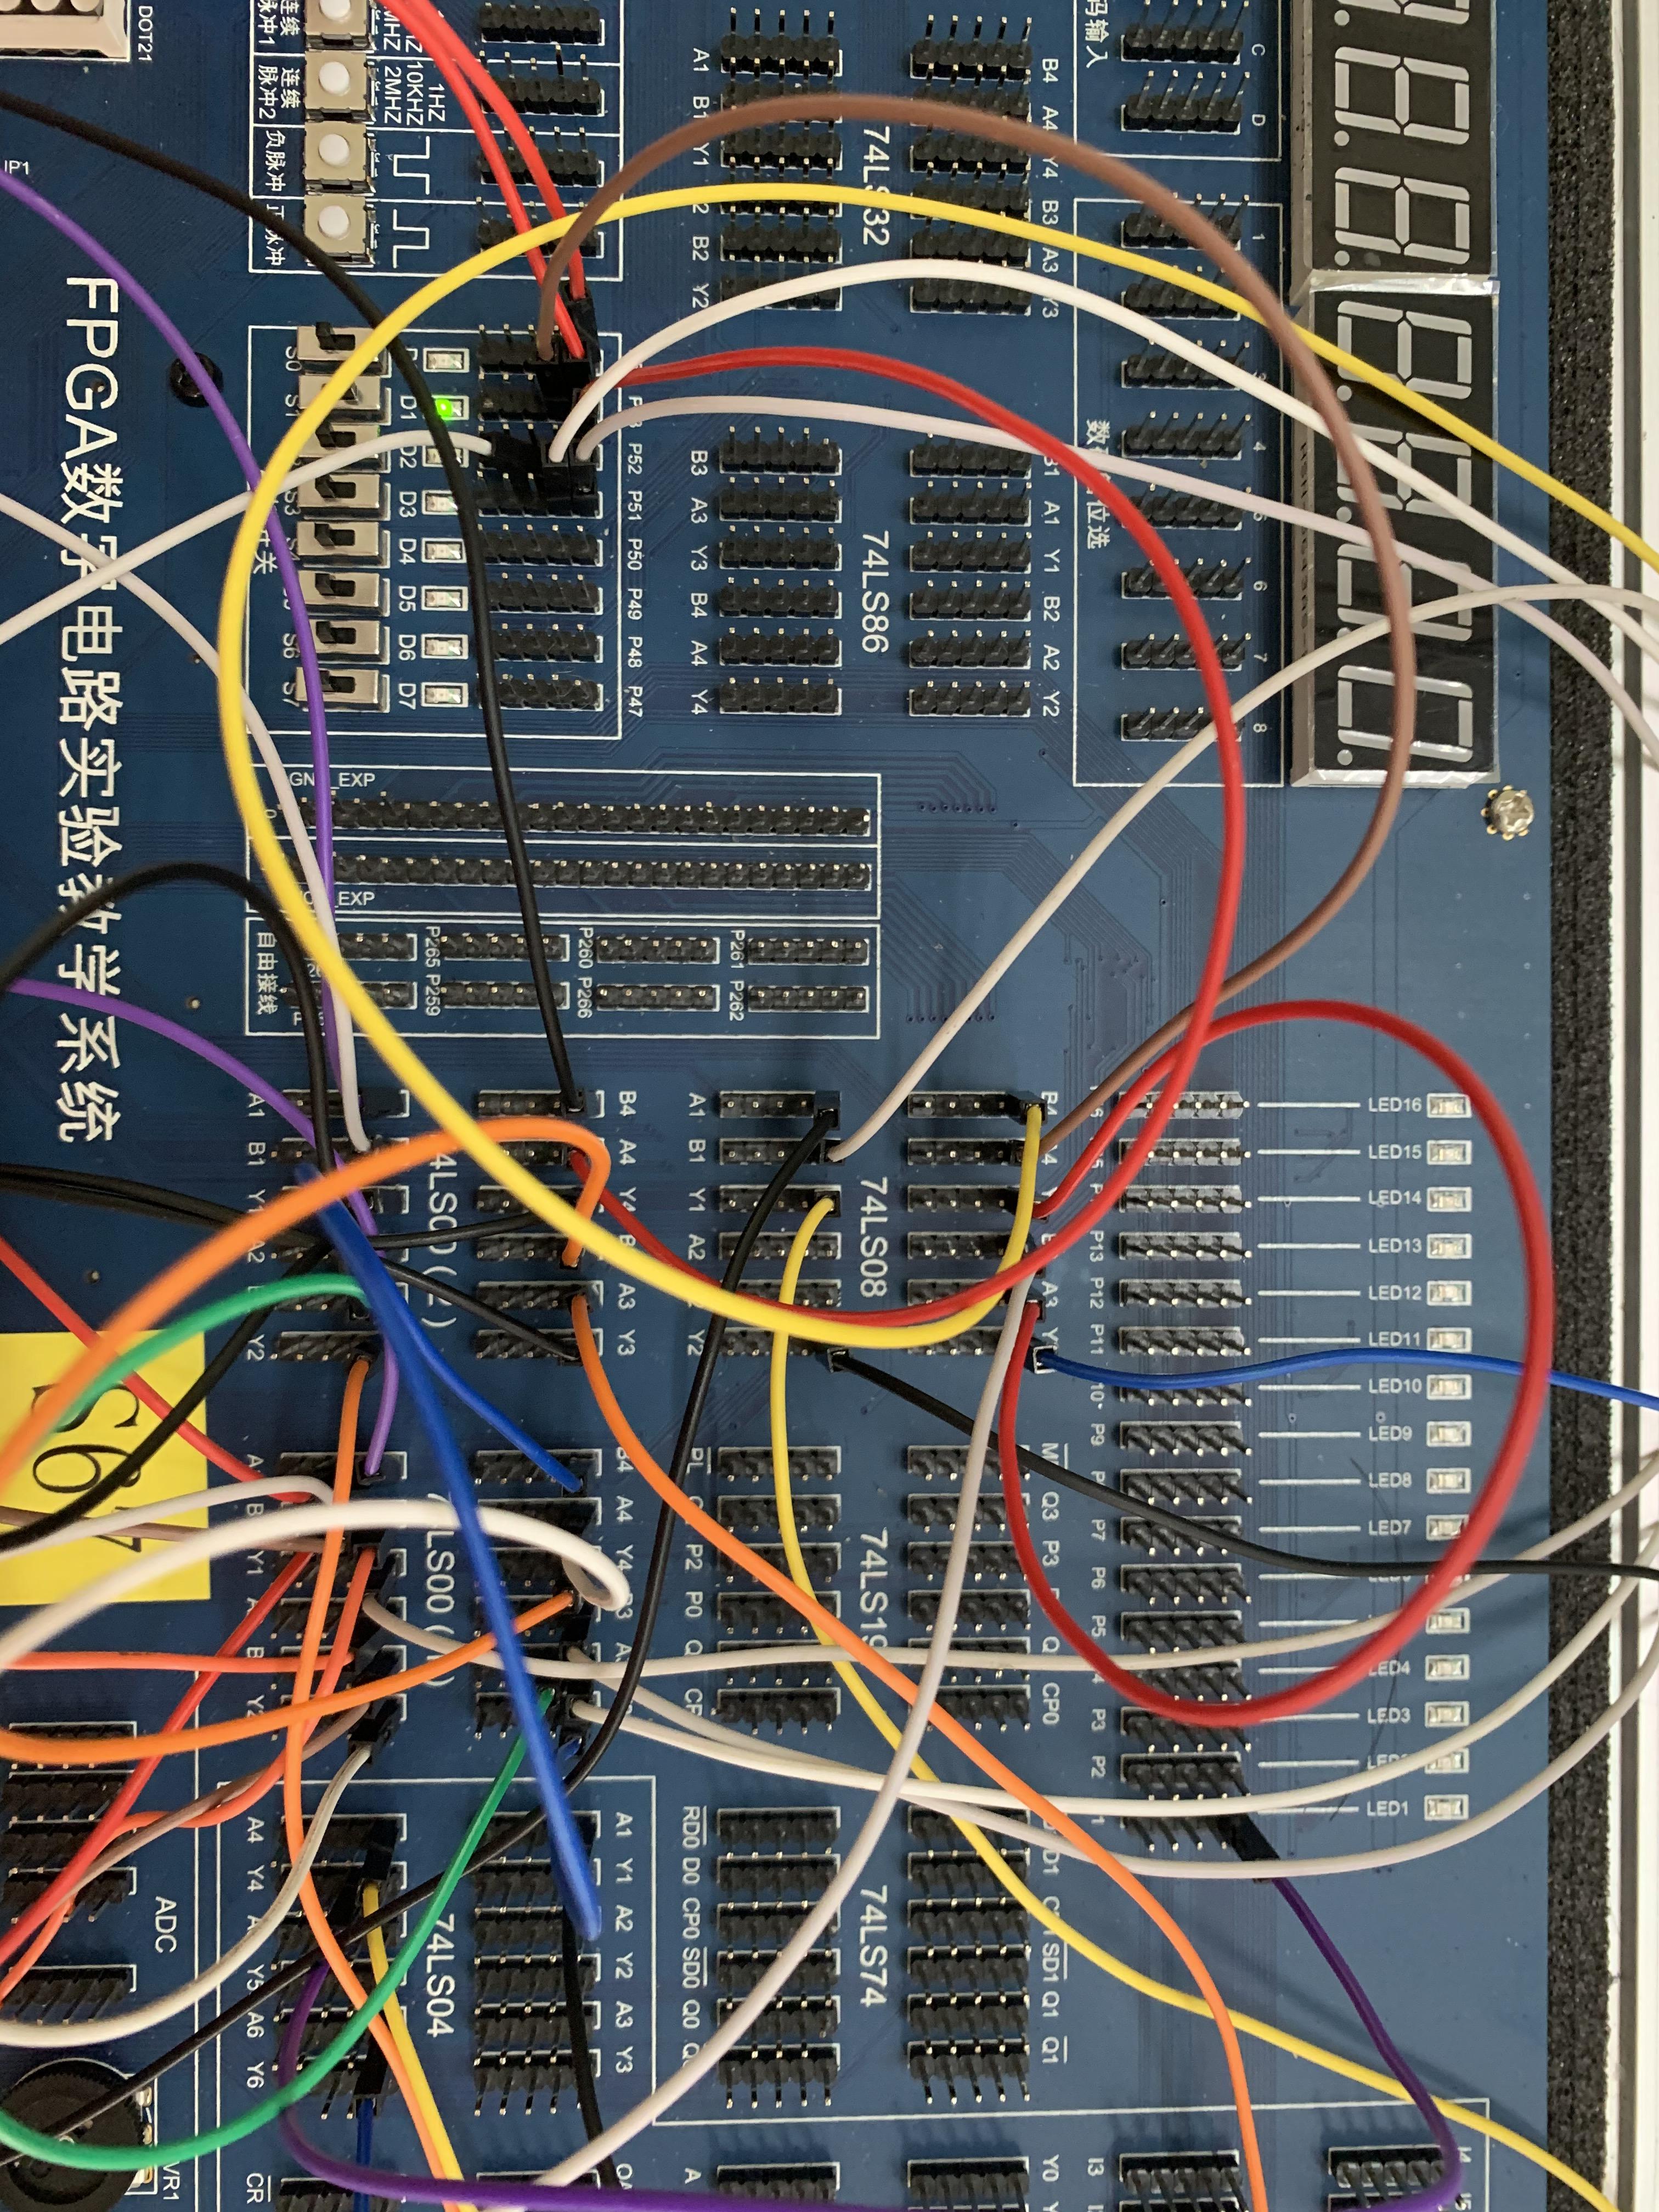
\includegraphics[width=0.8\textwidth]{0010.JPG}
\end{figure}
\begin{figure}[H]
    \centering
    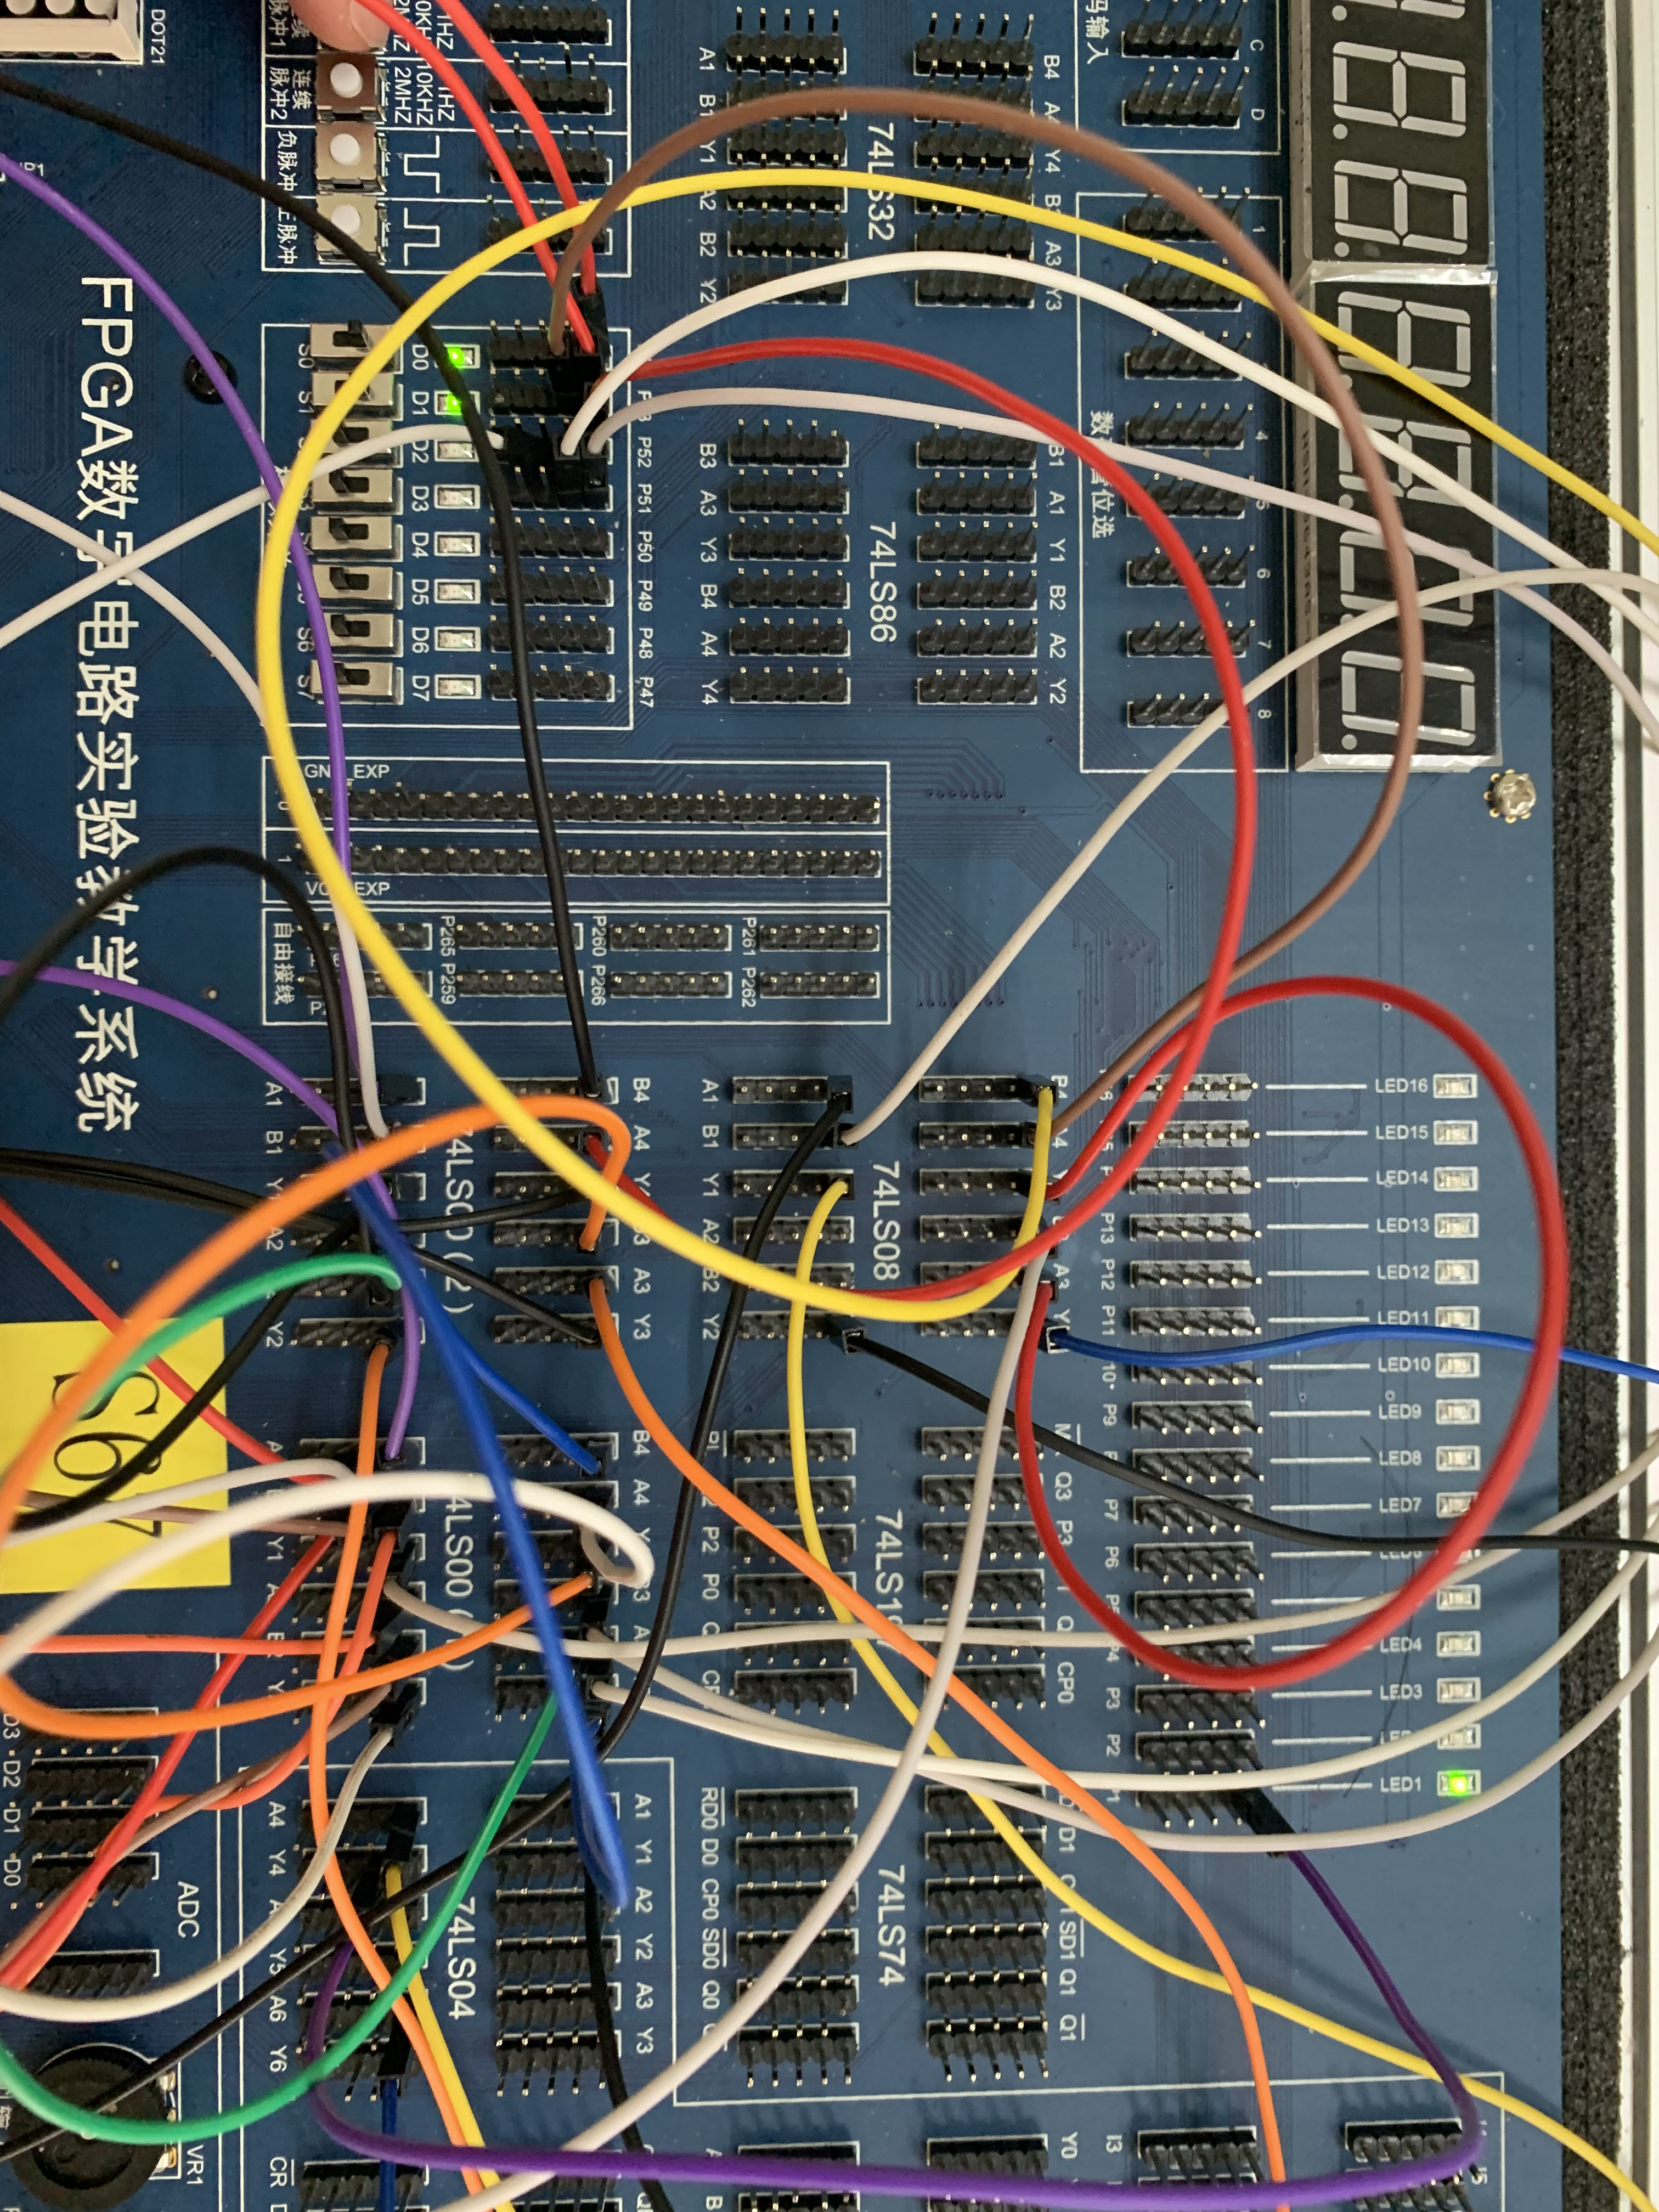
\includegraphics[width=0.8\textwidth]{0011.JPG}
\end{figure}
\begin{figure}[H]
    \centering
    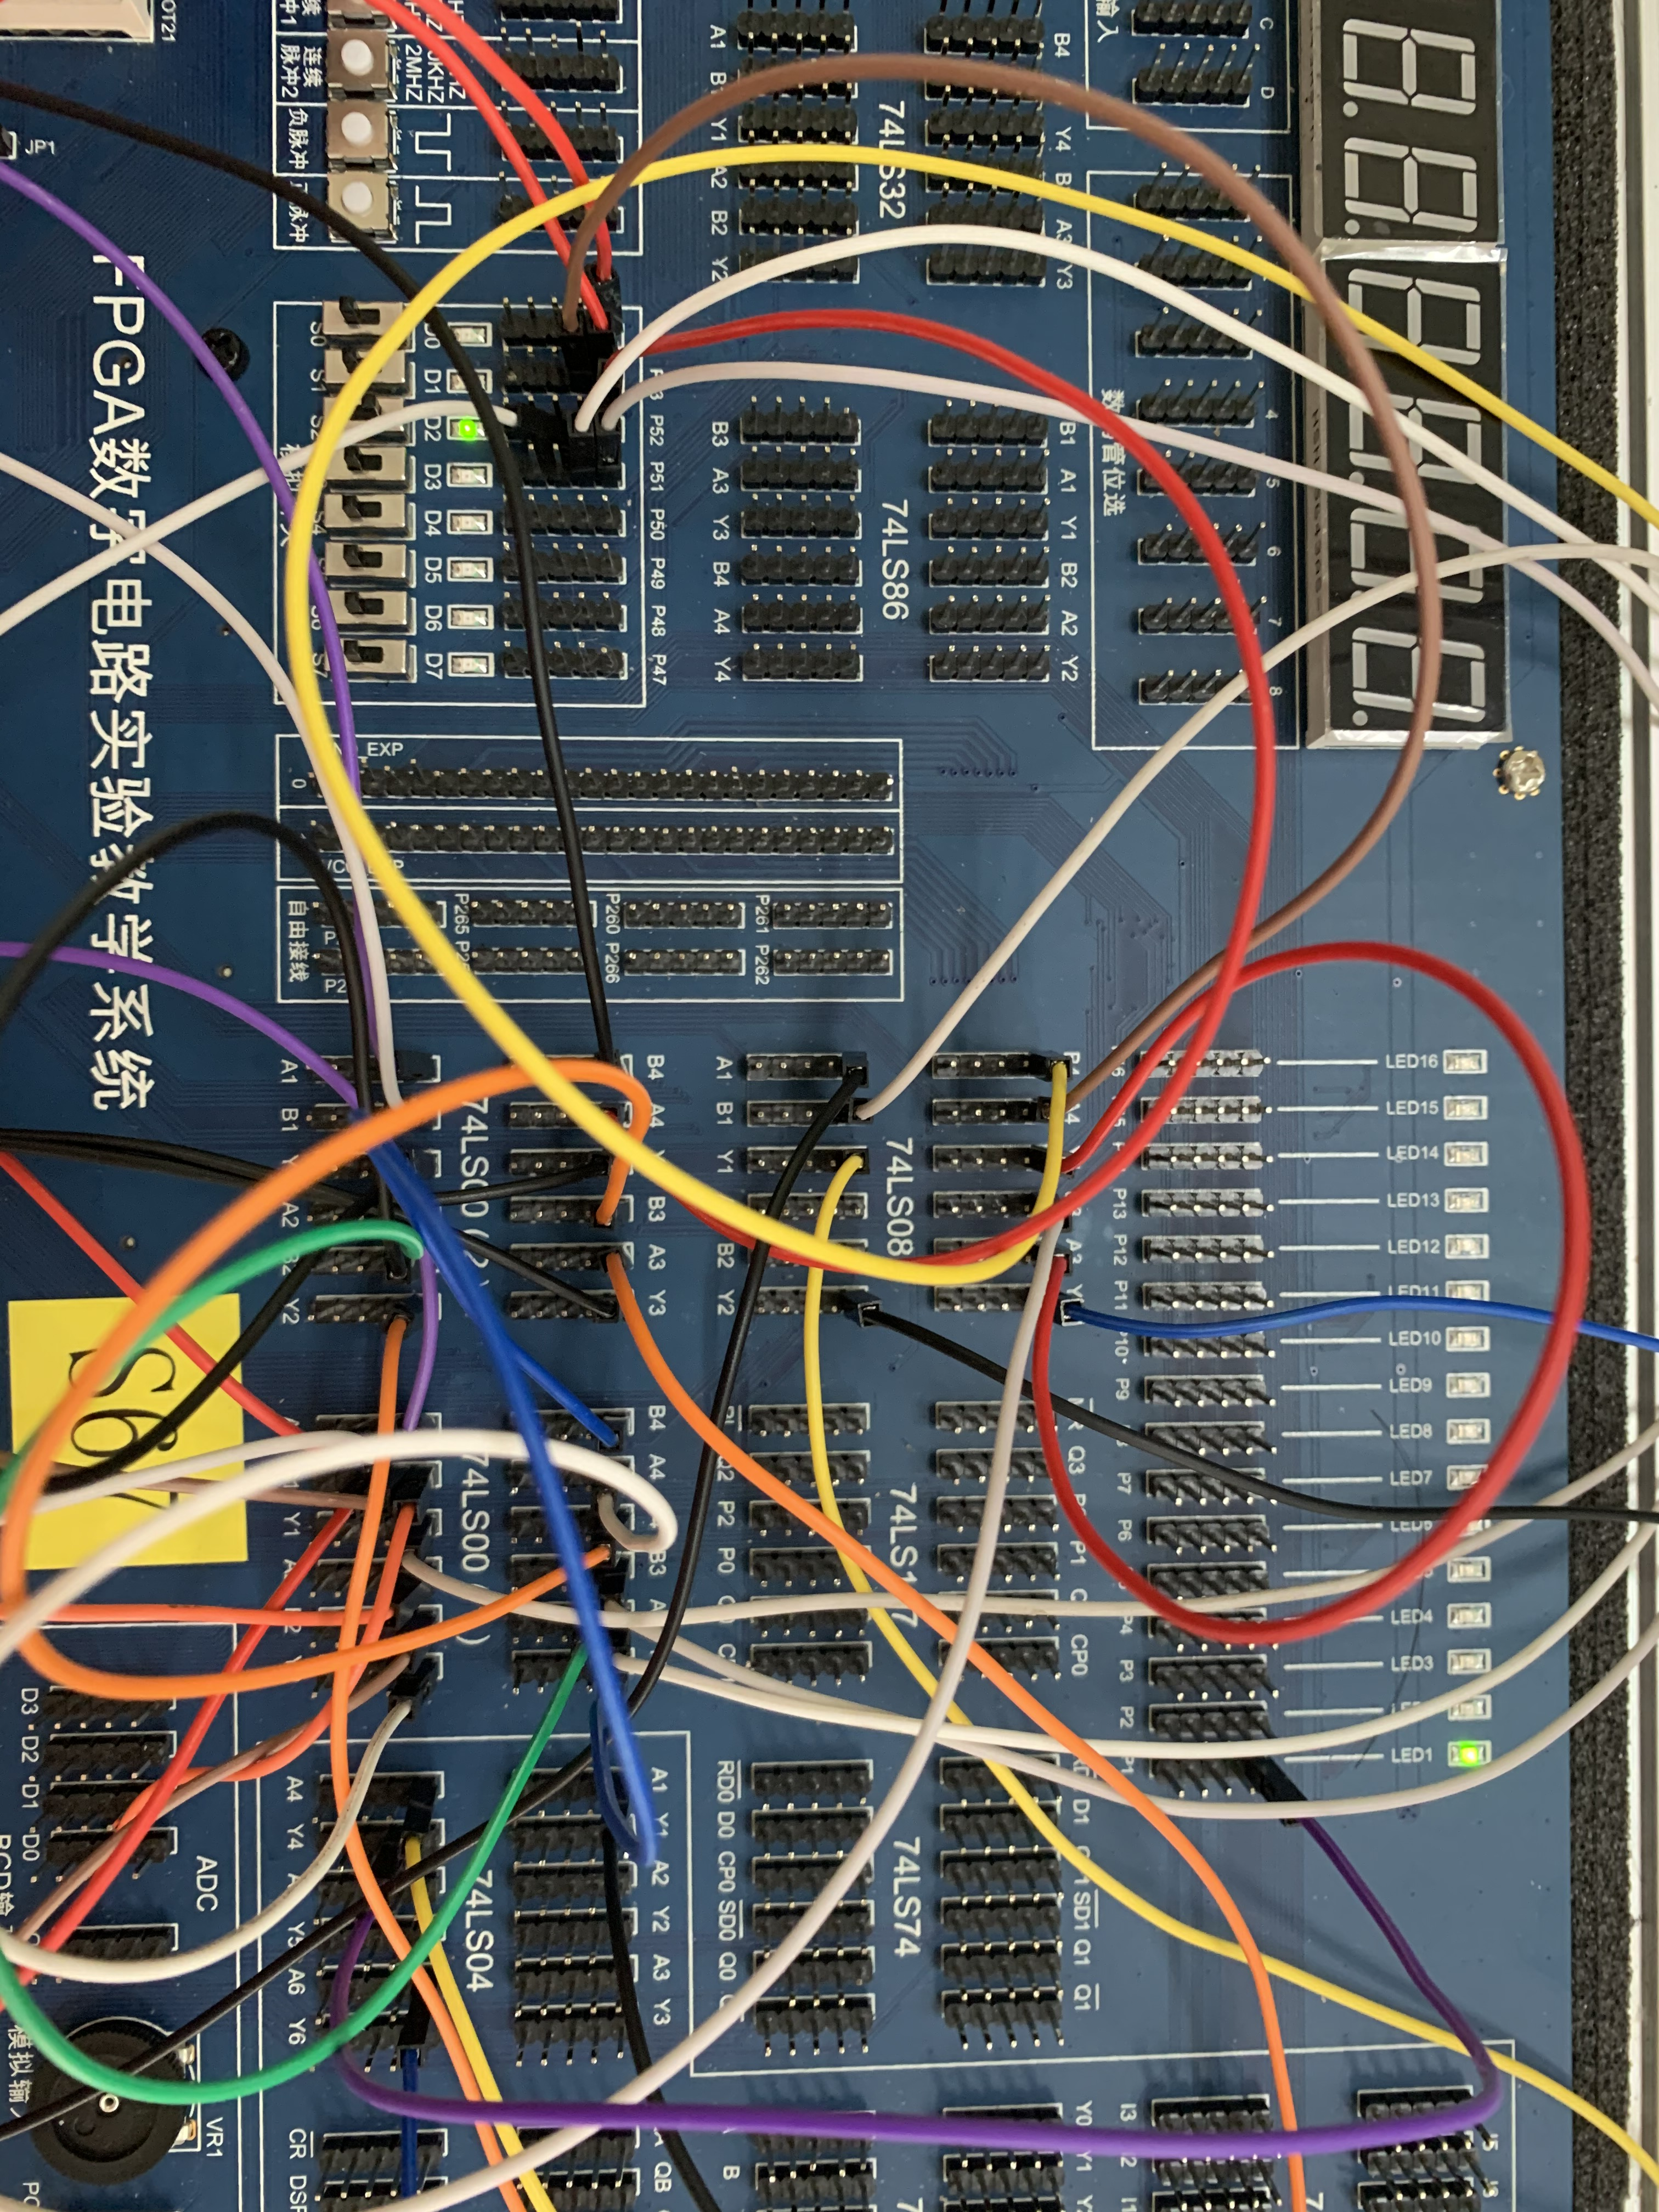
\includegraphics[width=0.8\textwidth]{0100.JPG}
\end{figure}
\begin{figure}[H]
    \centering
    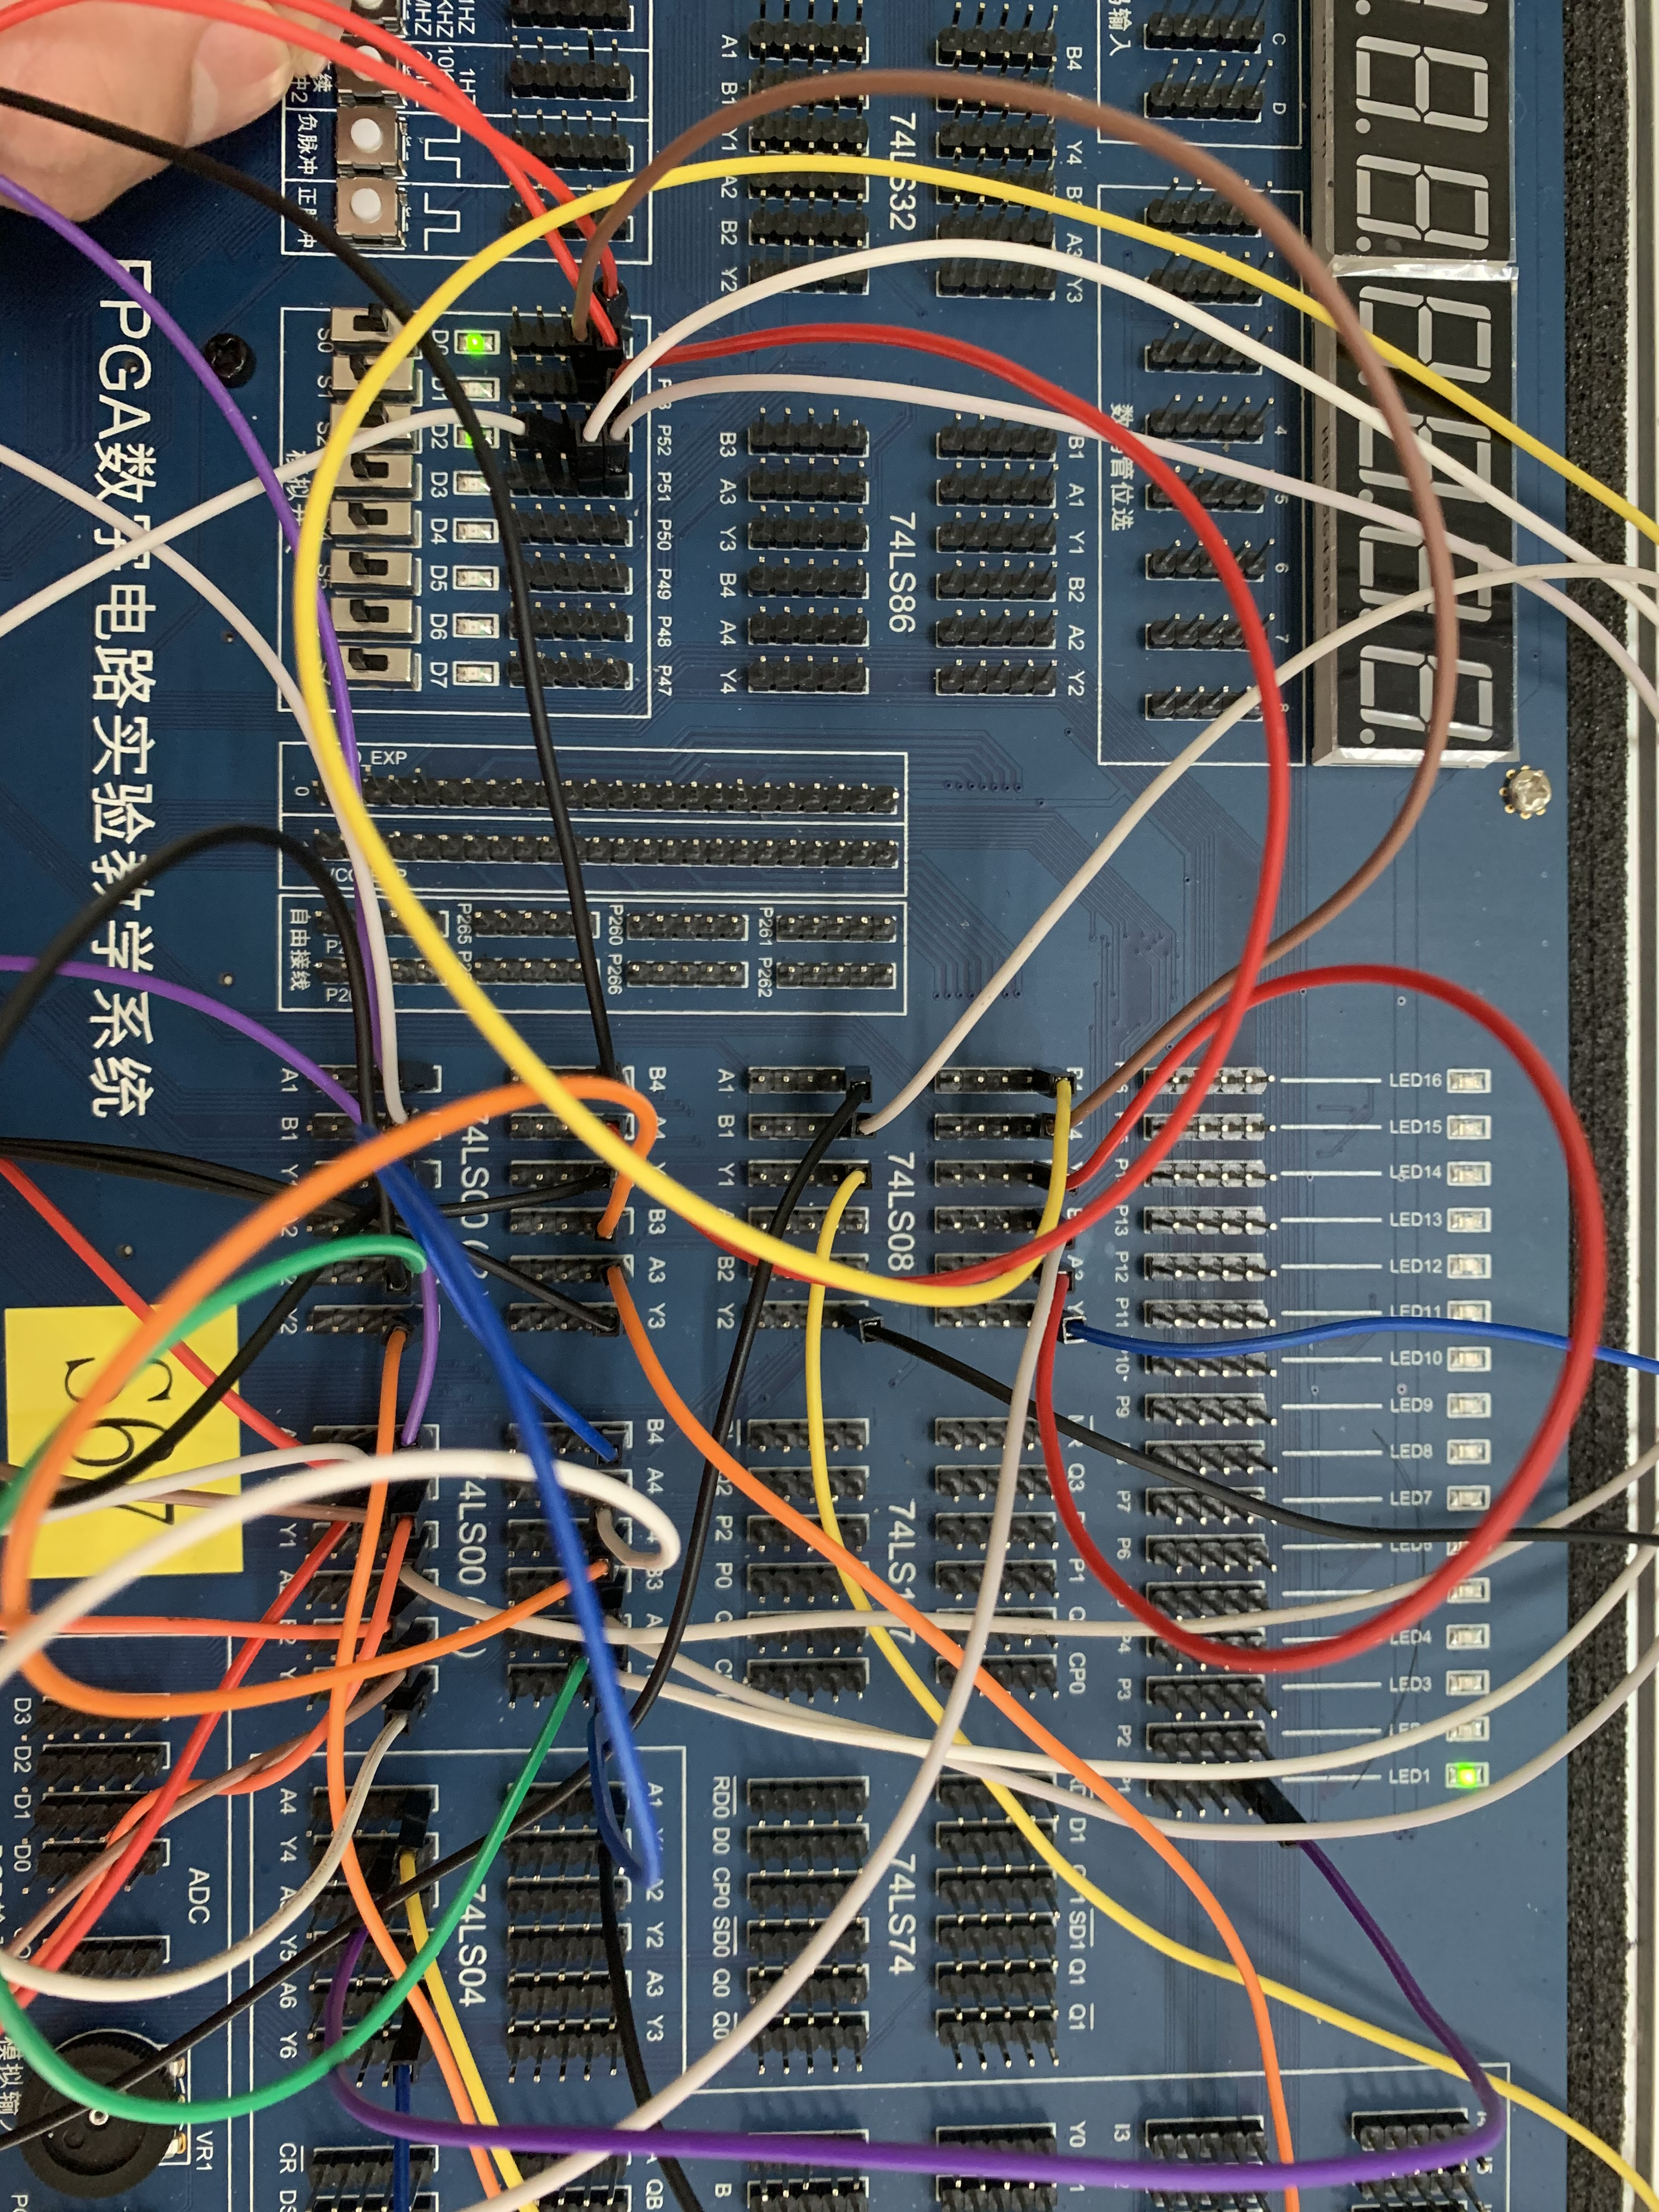
\includegraphics[width=0.8\textwidth]{0101.JPG}
\end{figure}
\begin{figure}[H]
    \centering
    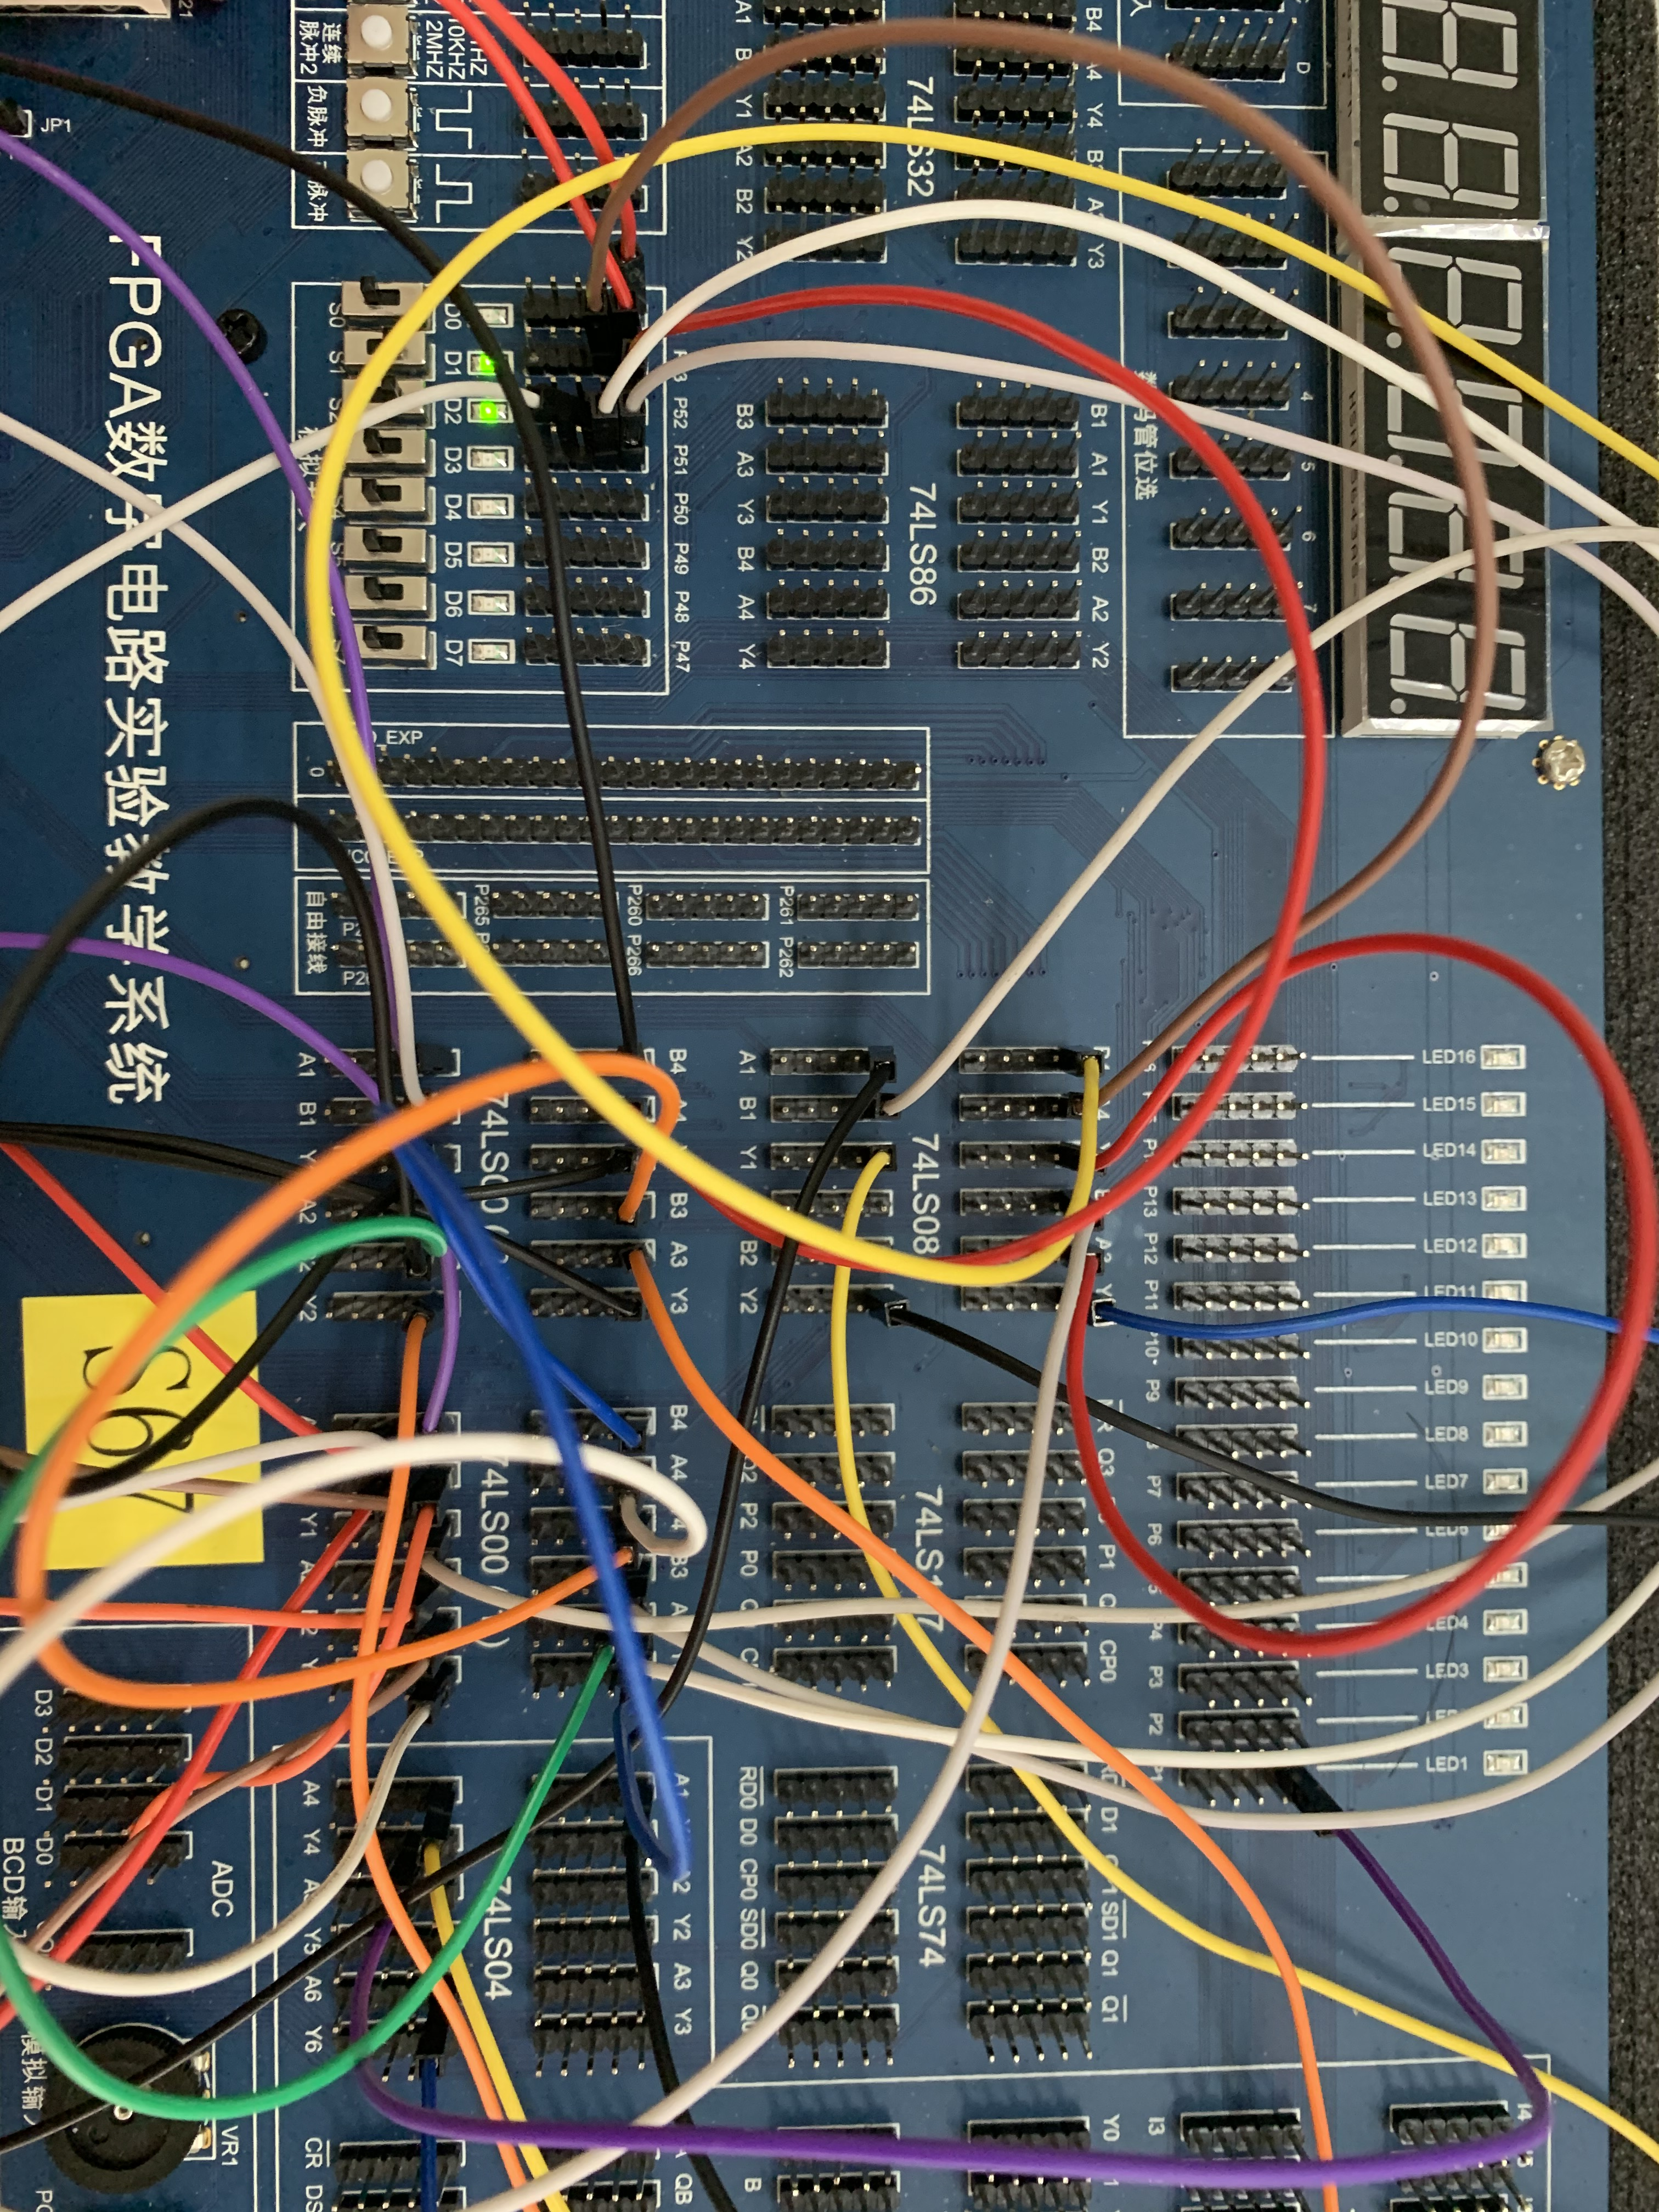
\includegraphics[width=0.8\textwidth]{0110.JPG}
\end{figure}
\begin{figure}[H]
    \centering
    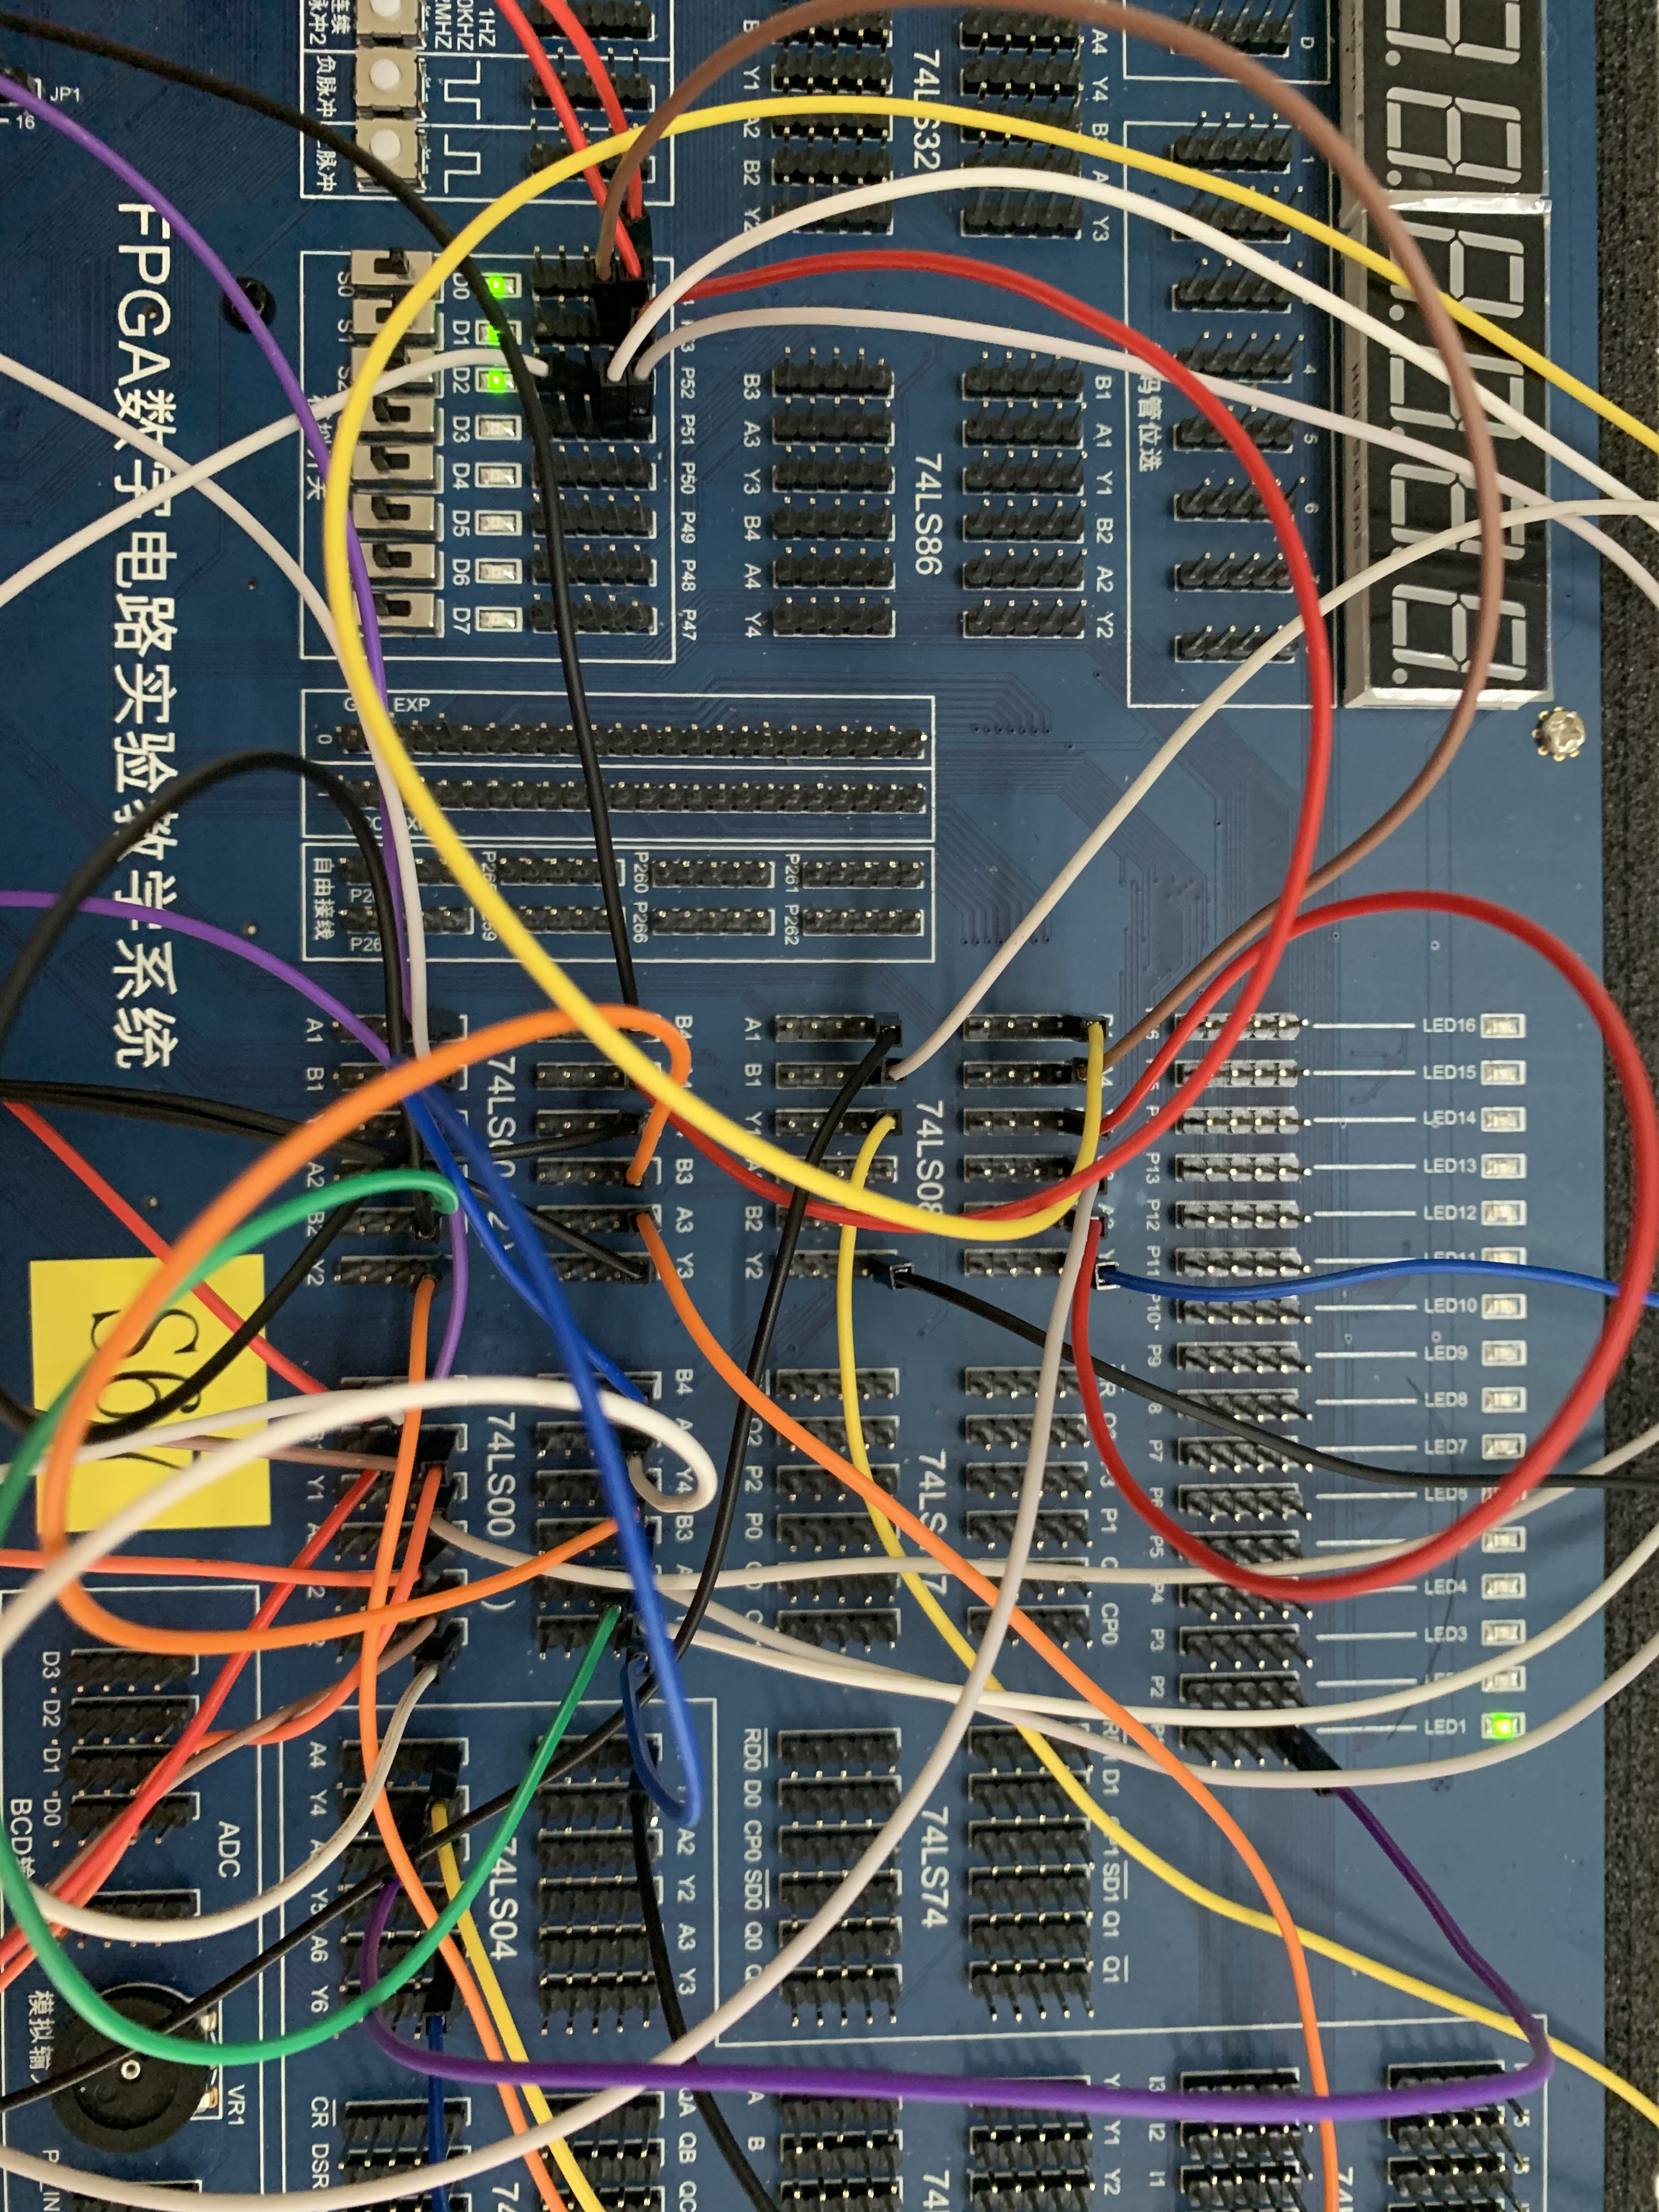
\includegraphics[width=0.8\textwidth]{0111.JPG}
\end{figure}
\begin{figure}[H]
    \centering
    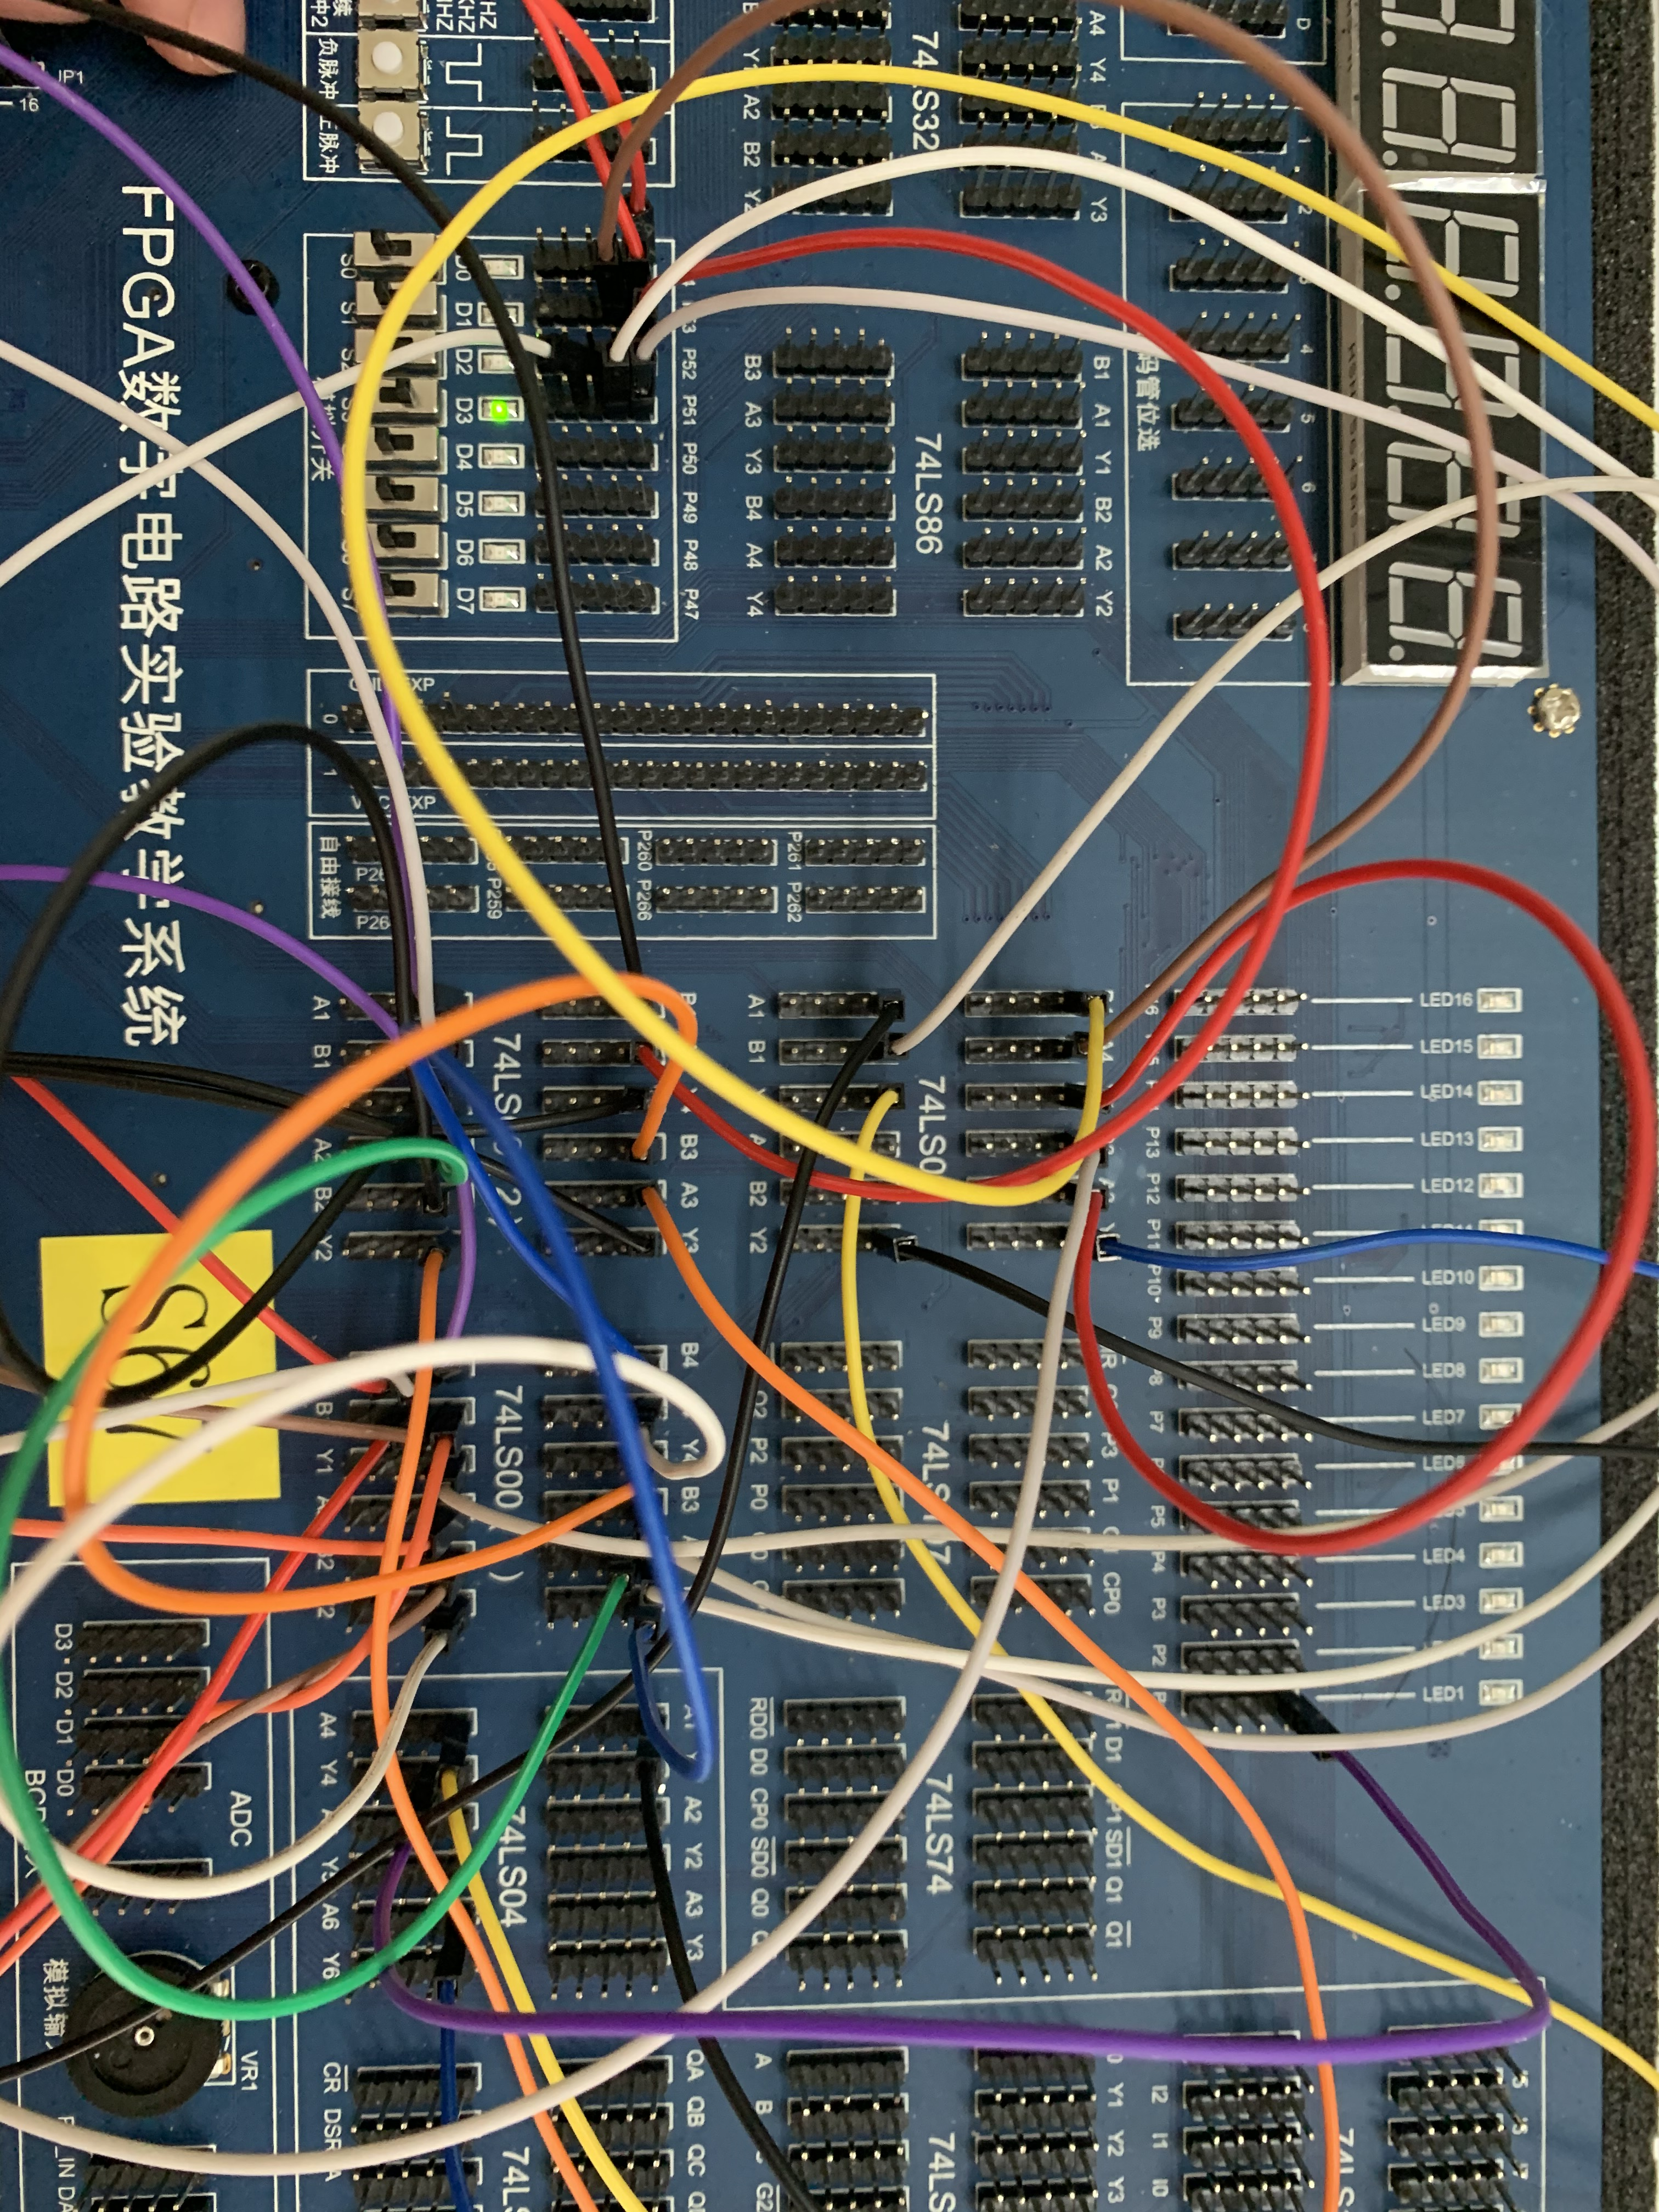
\includegraphics[width=0.8\textwidth]{1000.JPG}
\end{figure}
\begin{figure}[H]
    \centering
    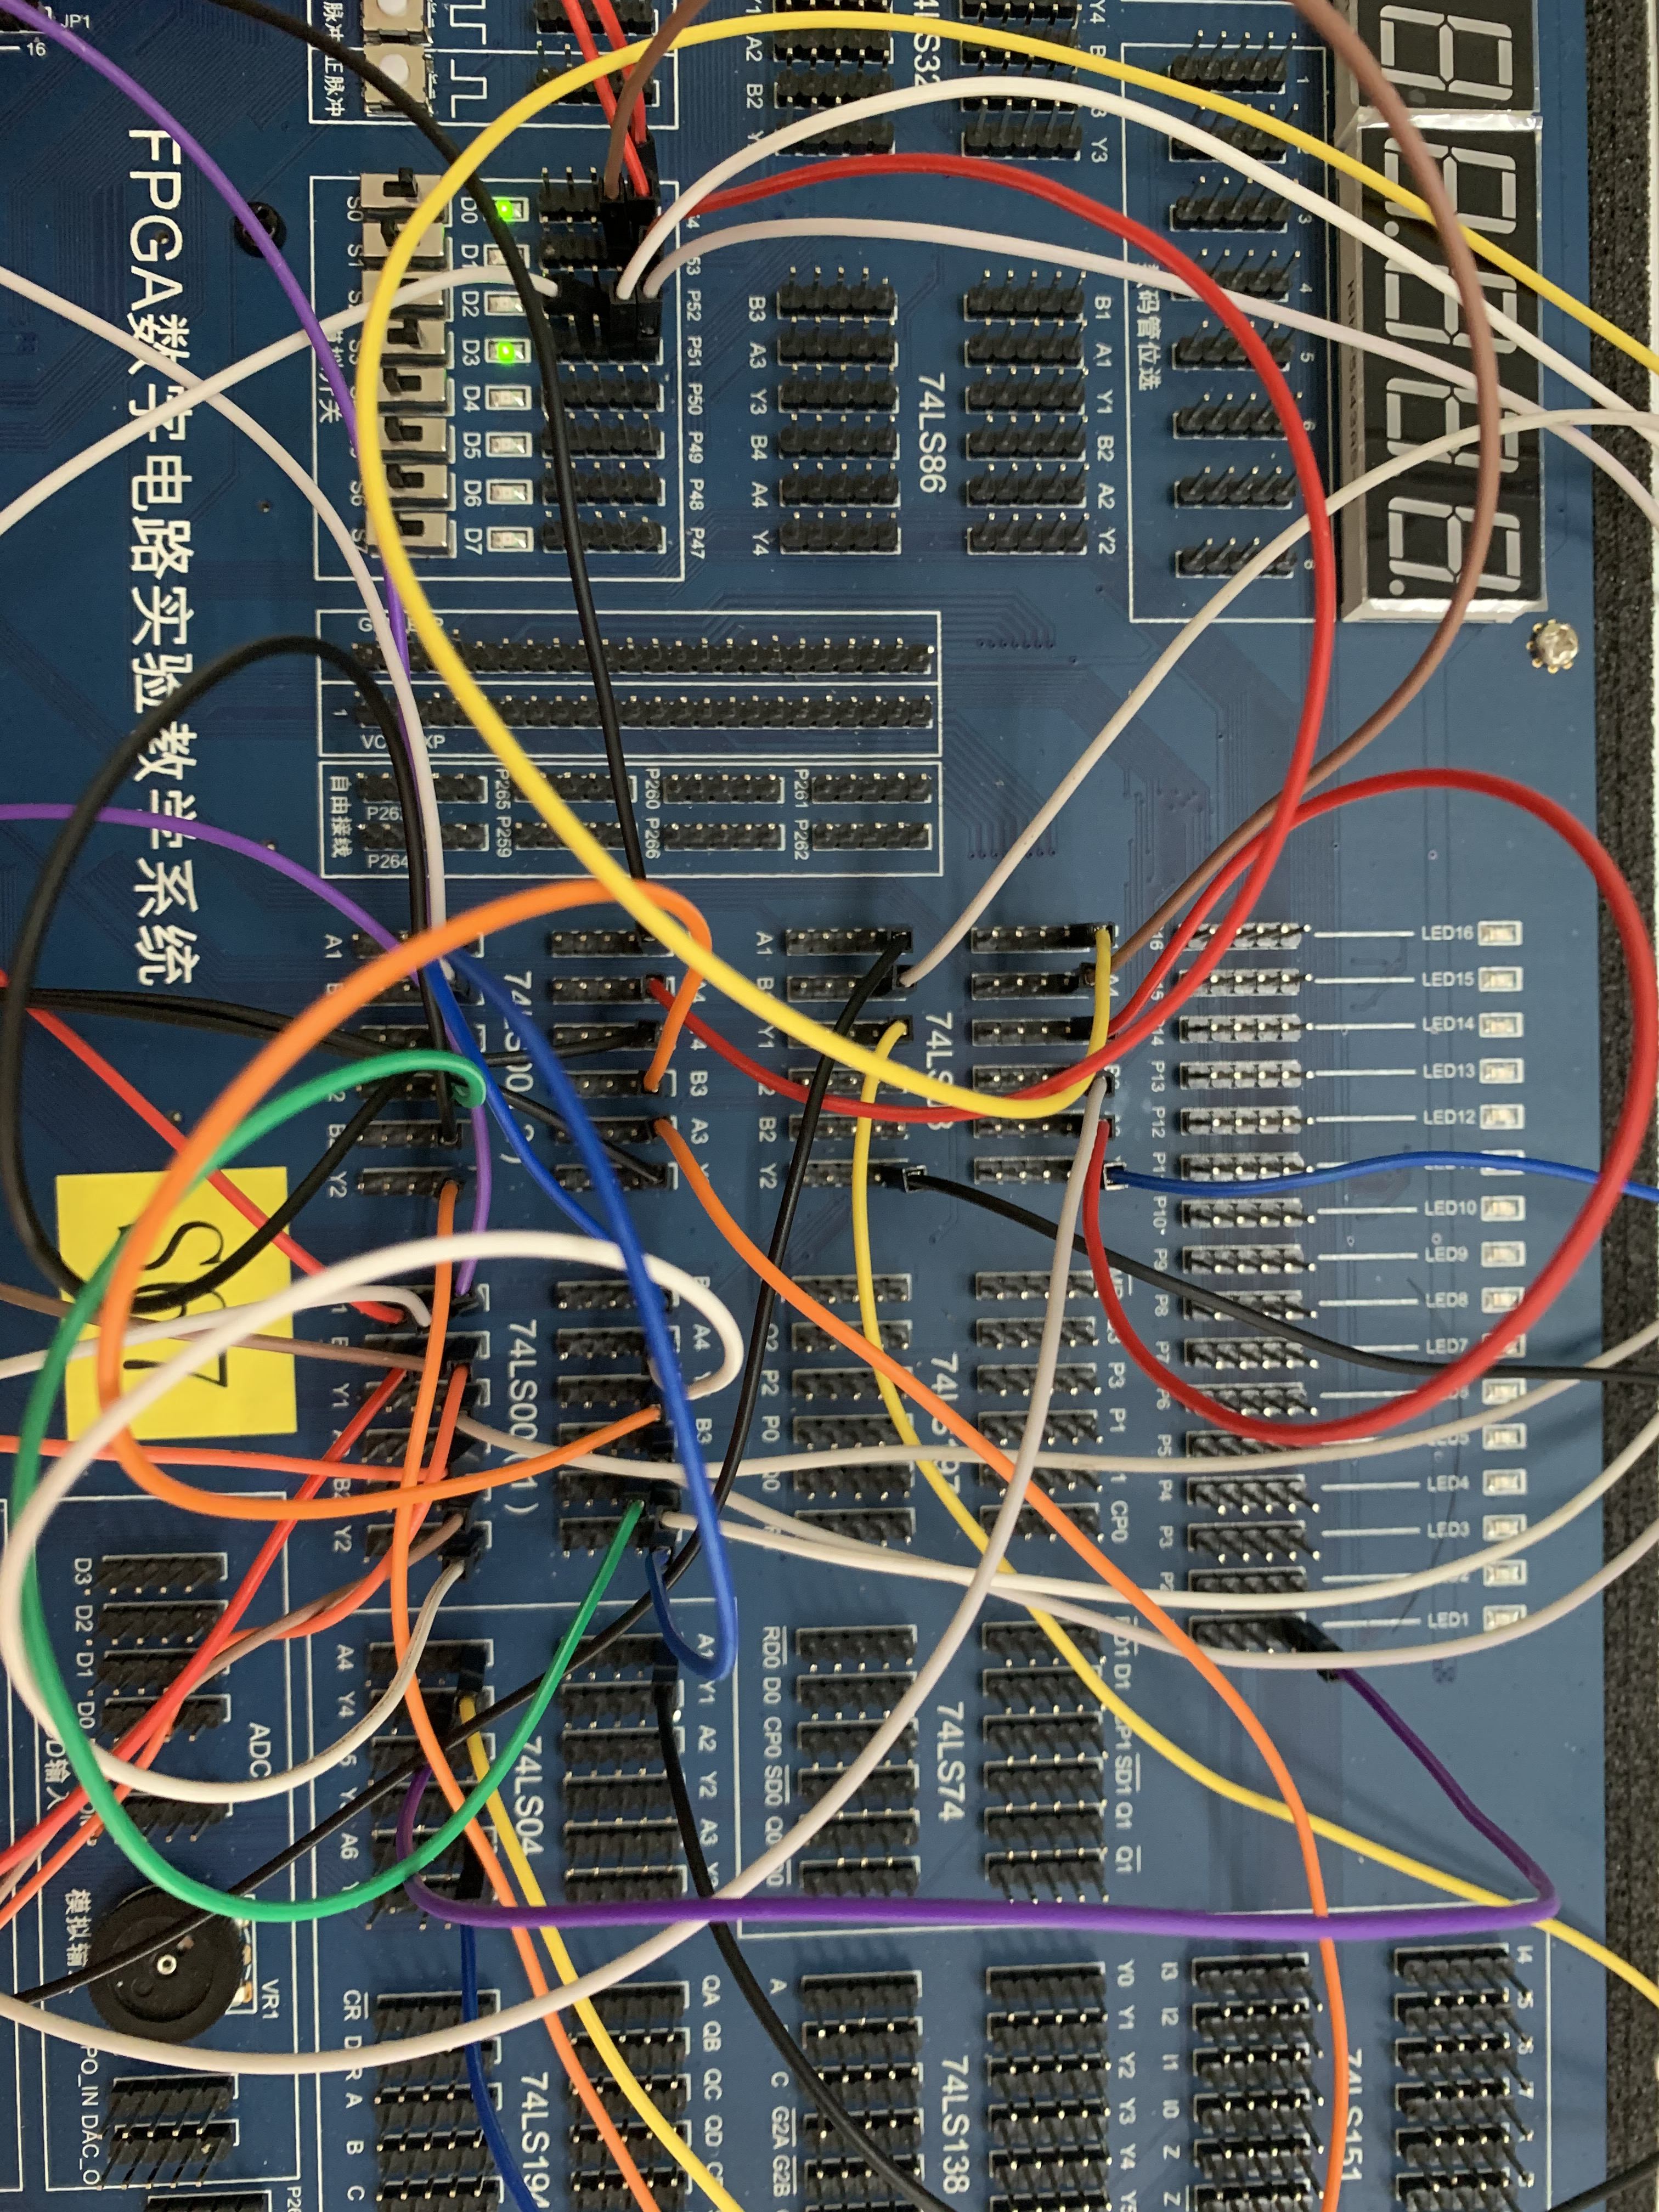
\includegraphics[width=0.8\textwidth]{1001.JPG}
\end{figure}
\begin{figure}[H]
    \centering
    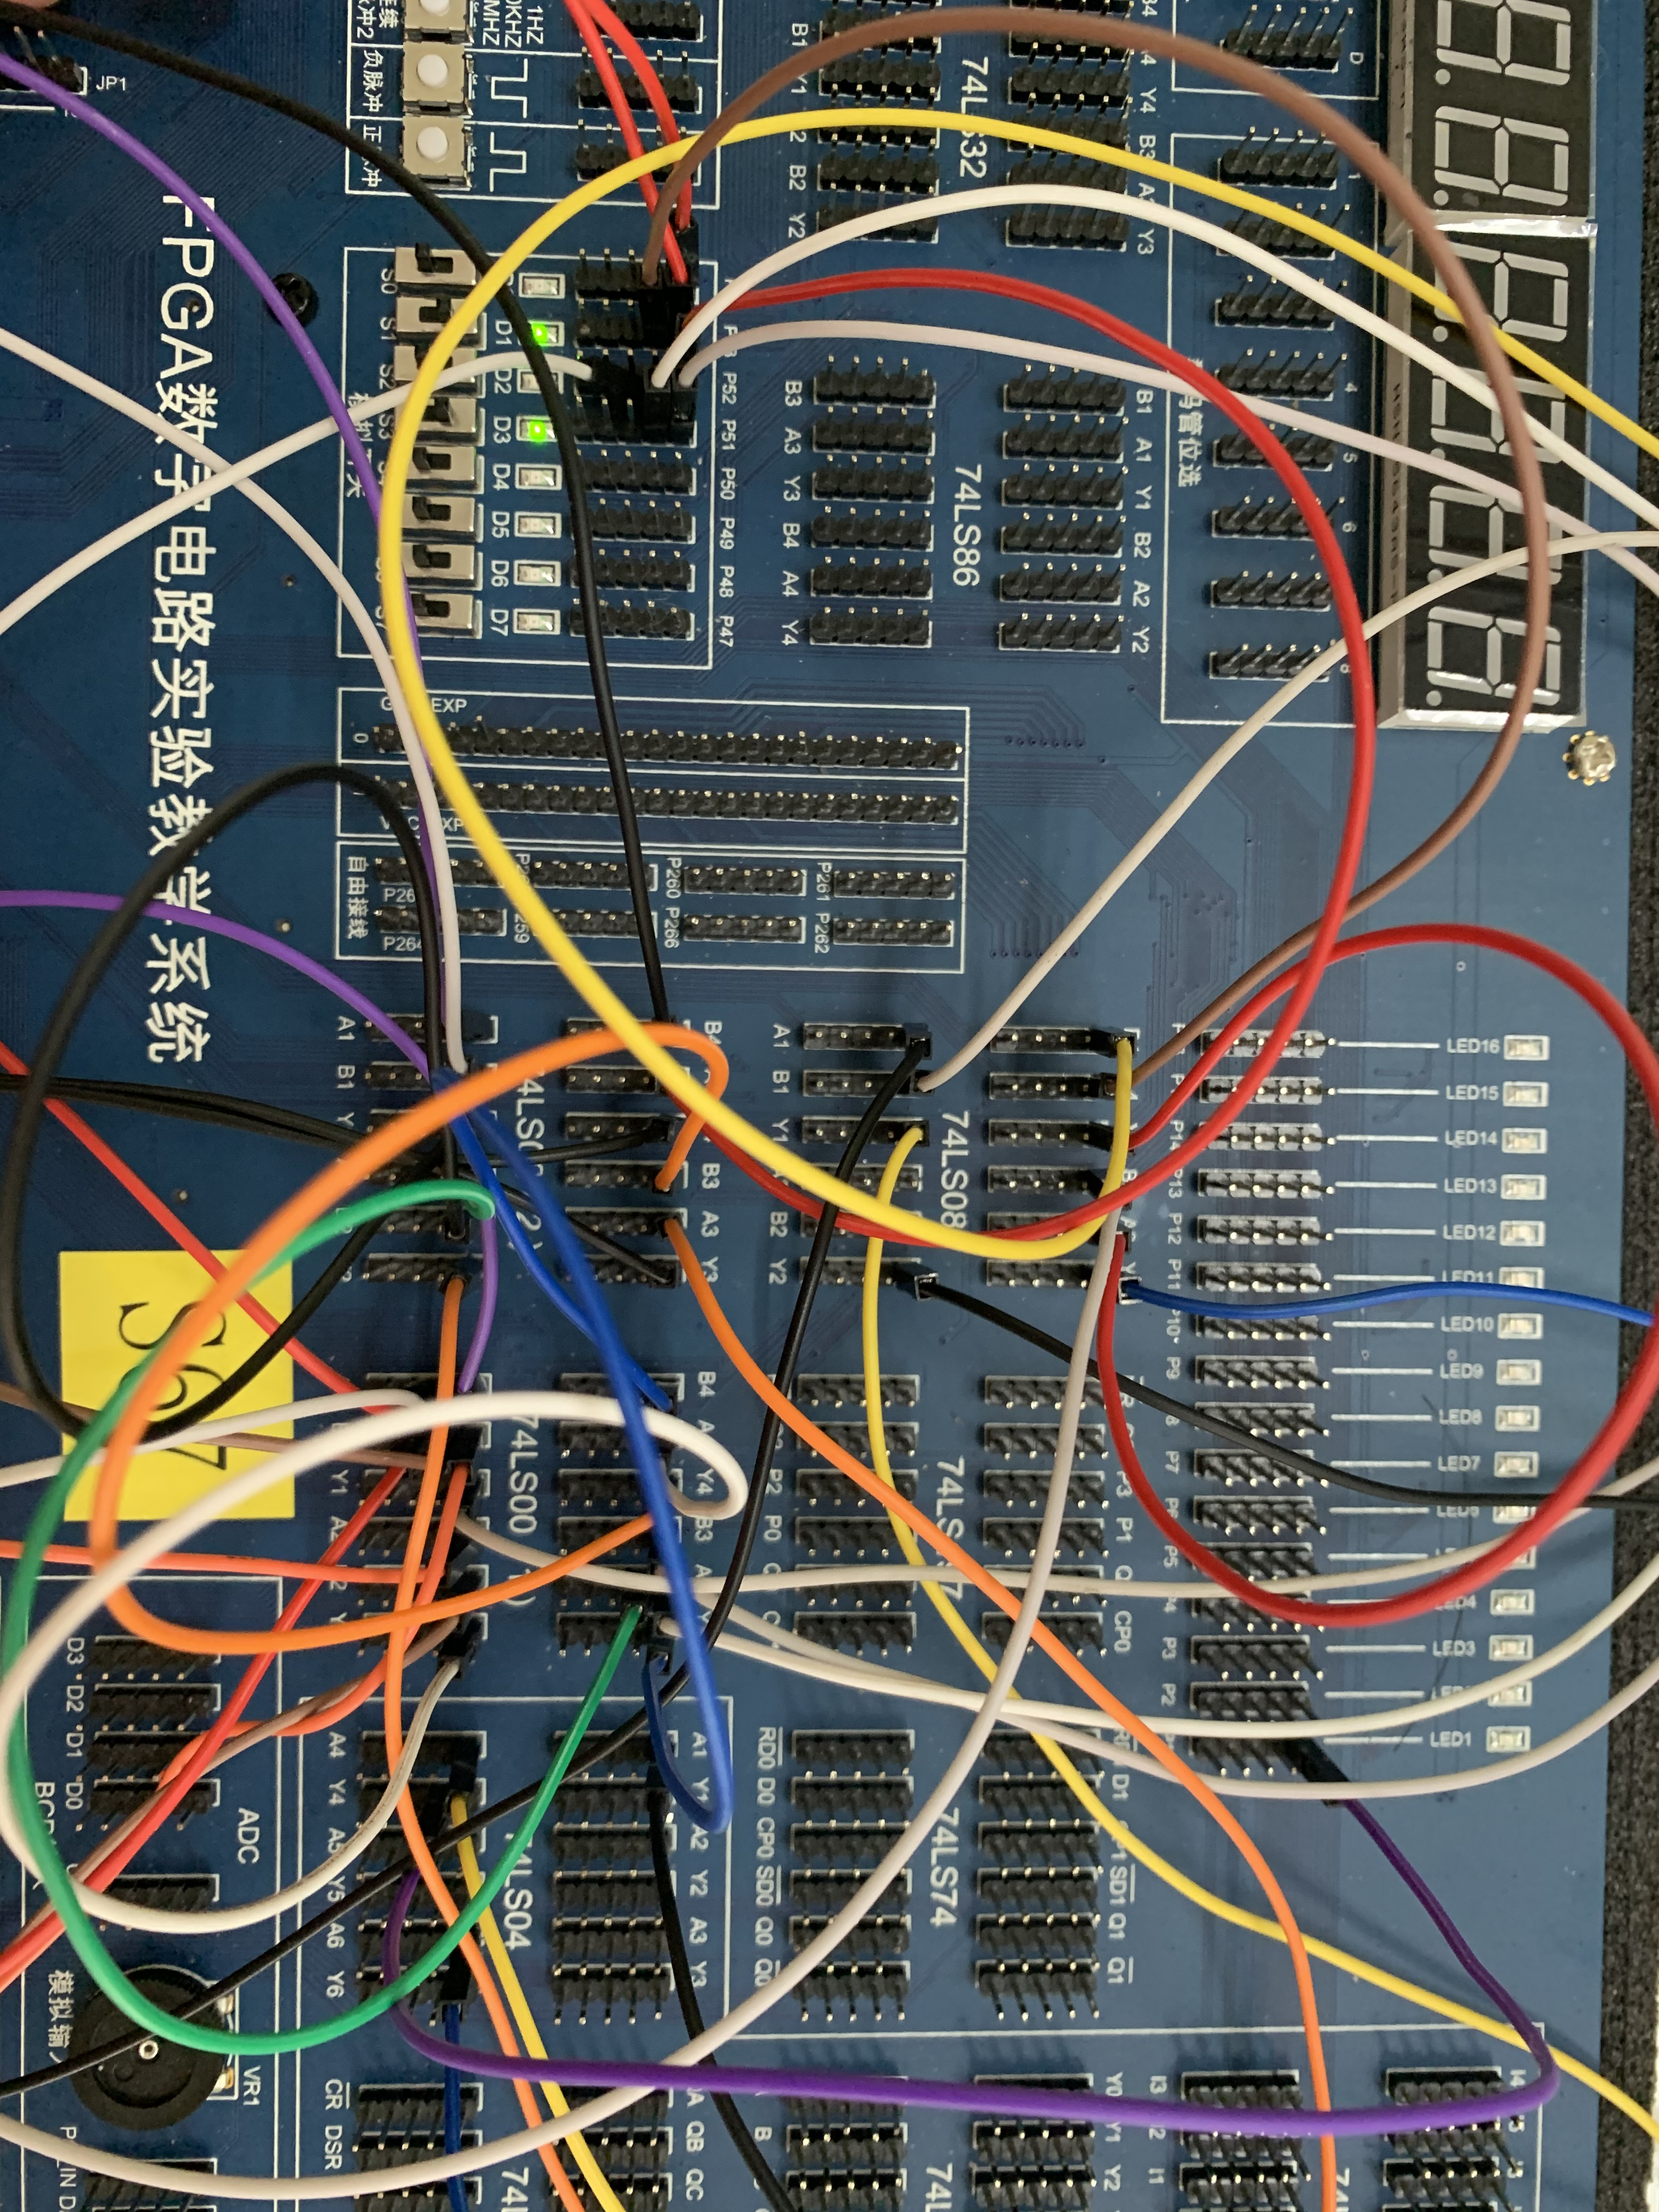
\includegraphics[width=0.8\textwidth]{1010.JPG}
\end{figure}
\begin{figure}[H]
    \centering
    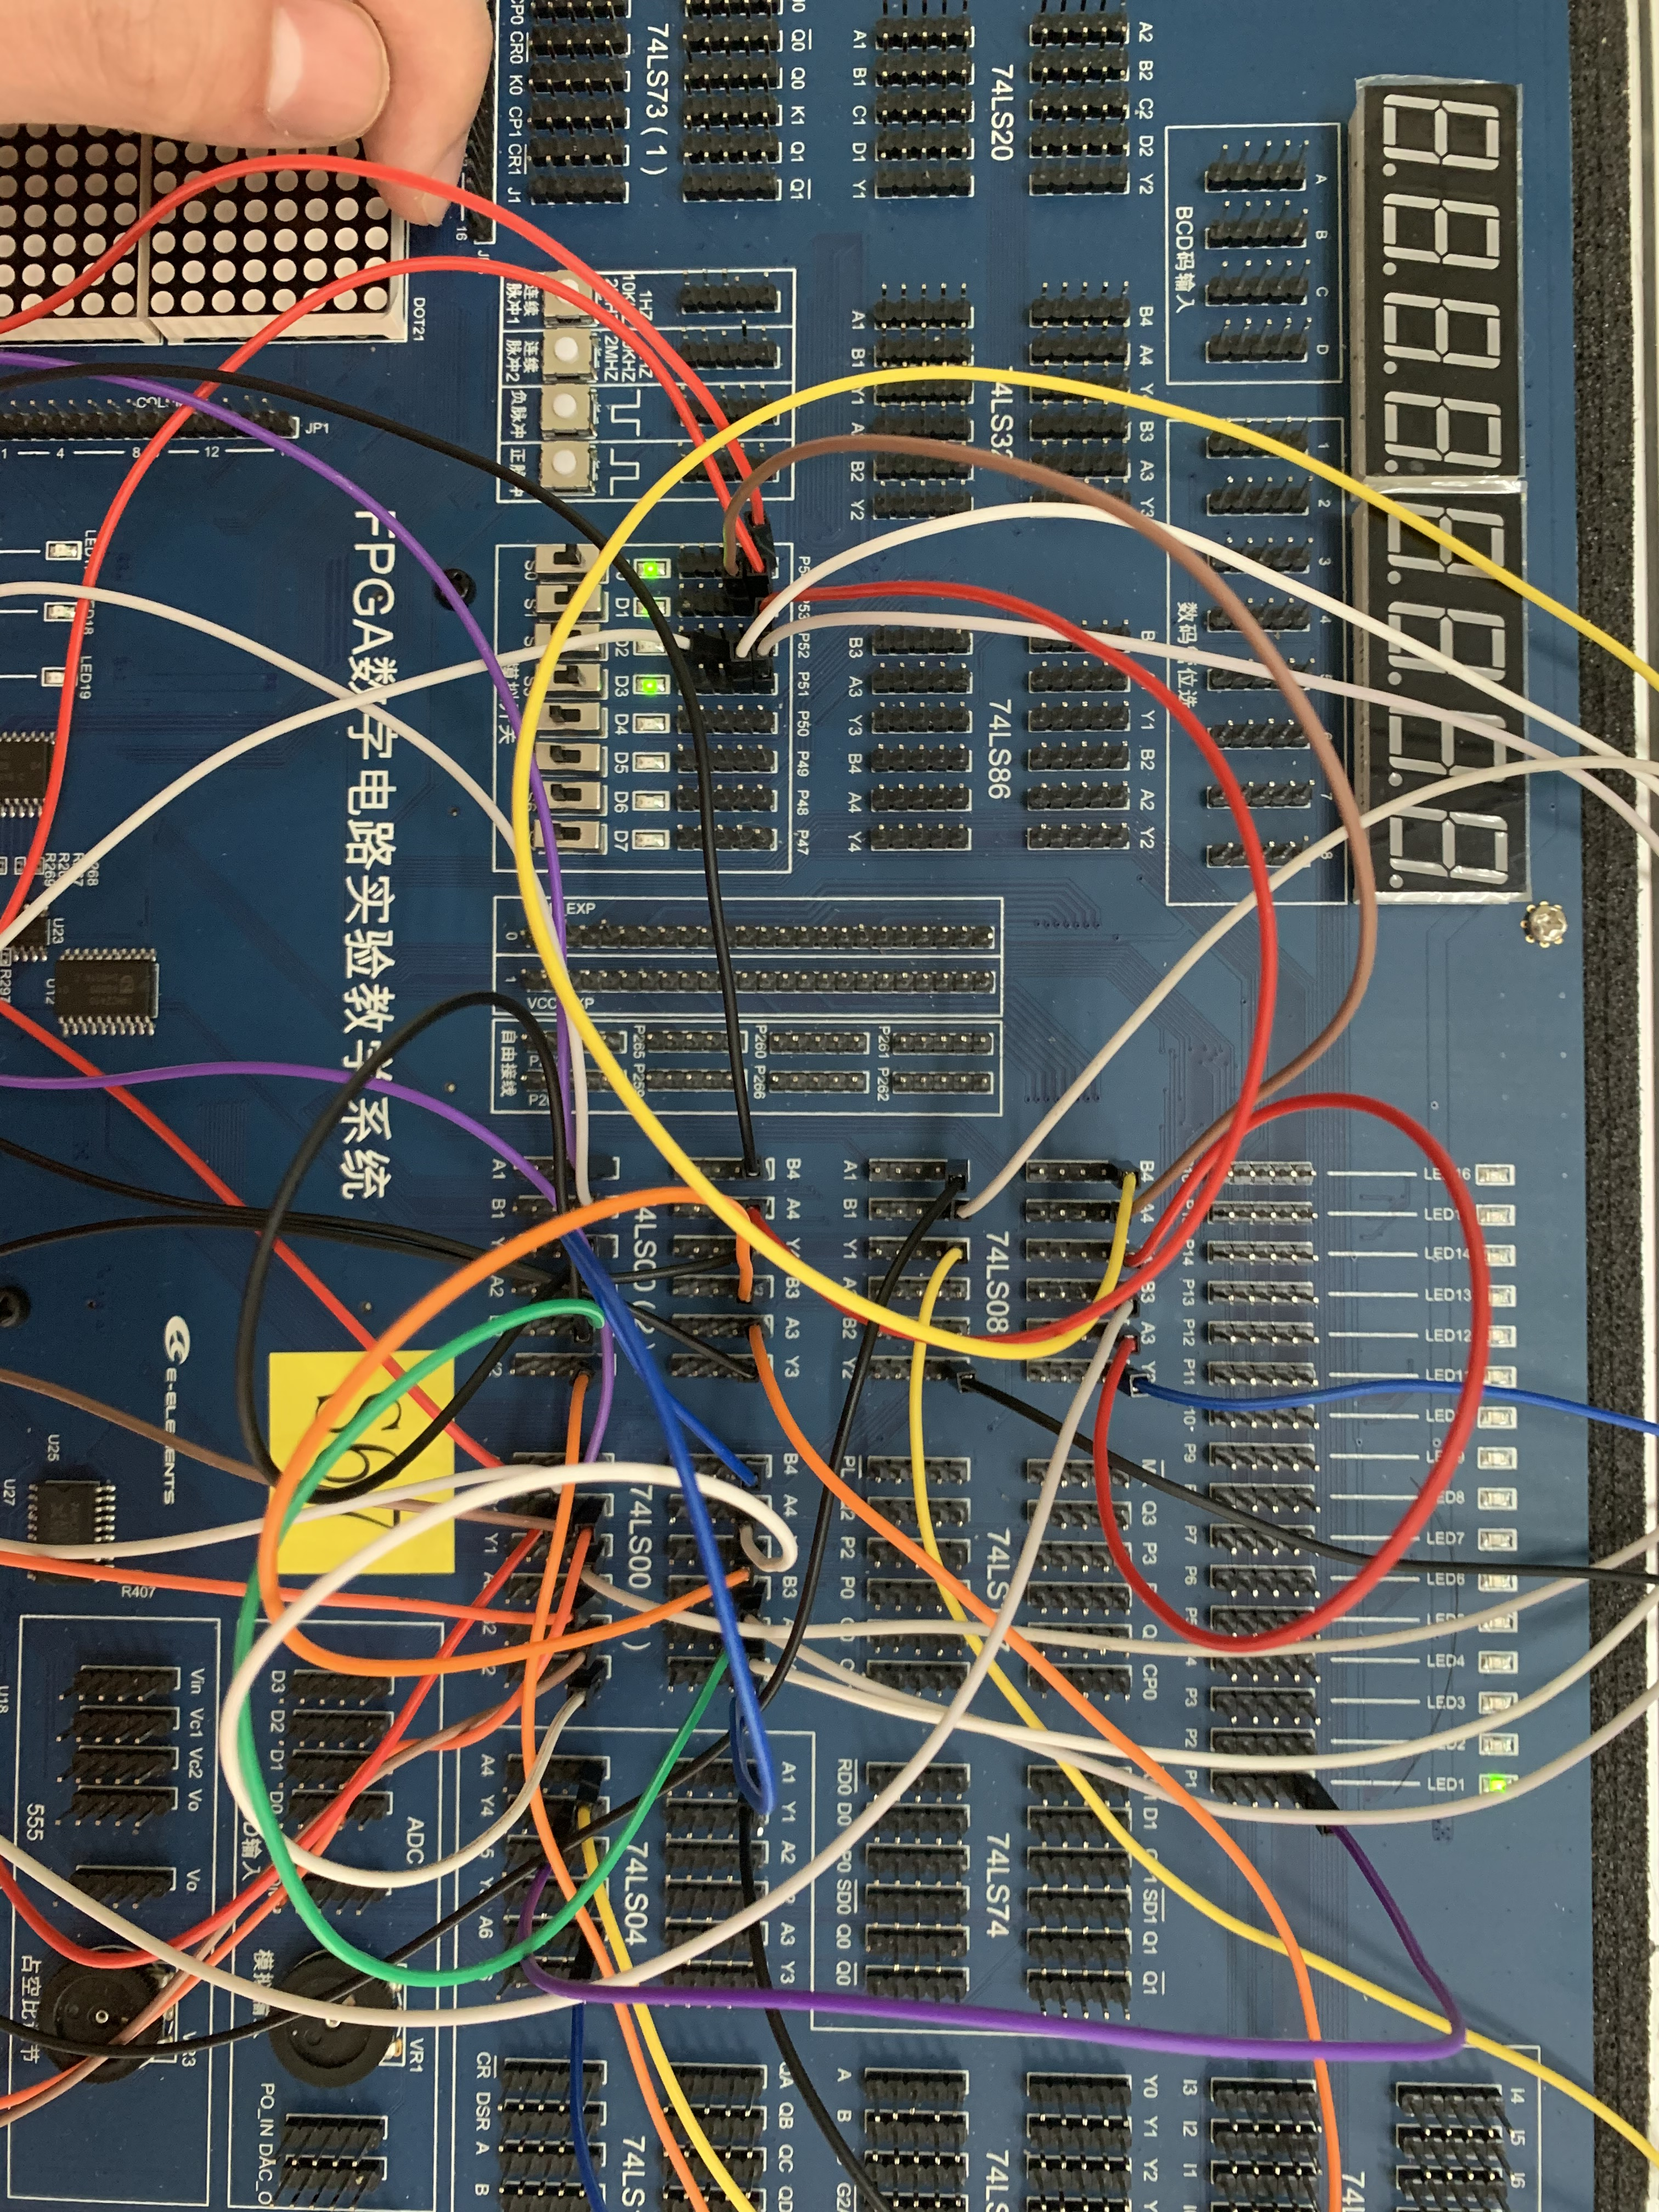
\includegraphics[width=0.8\textwidth]{1011.JPG}
\end{figure}
\begin{figure}[H]
    \centering
    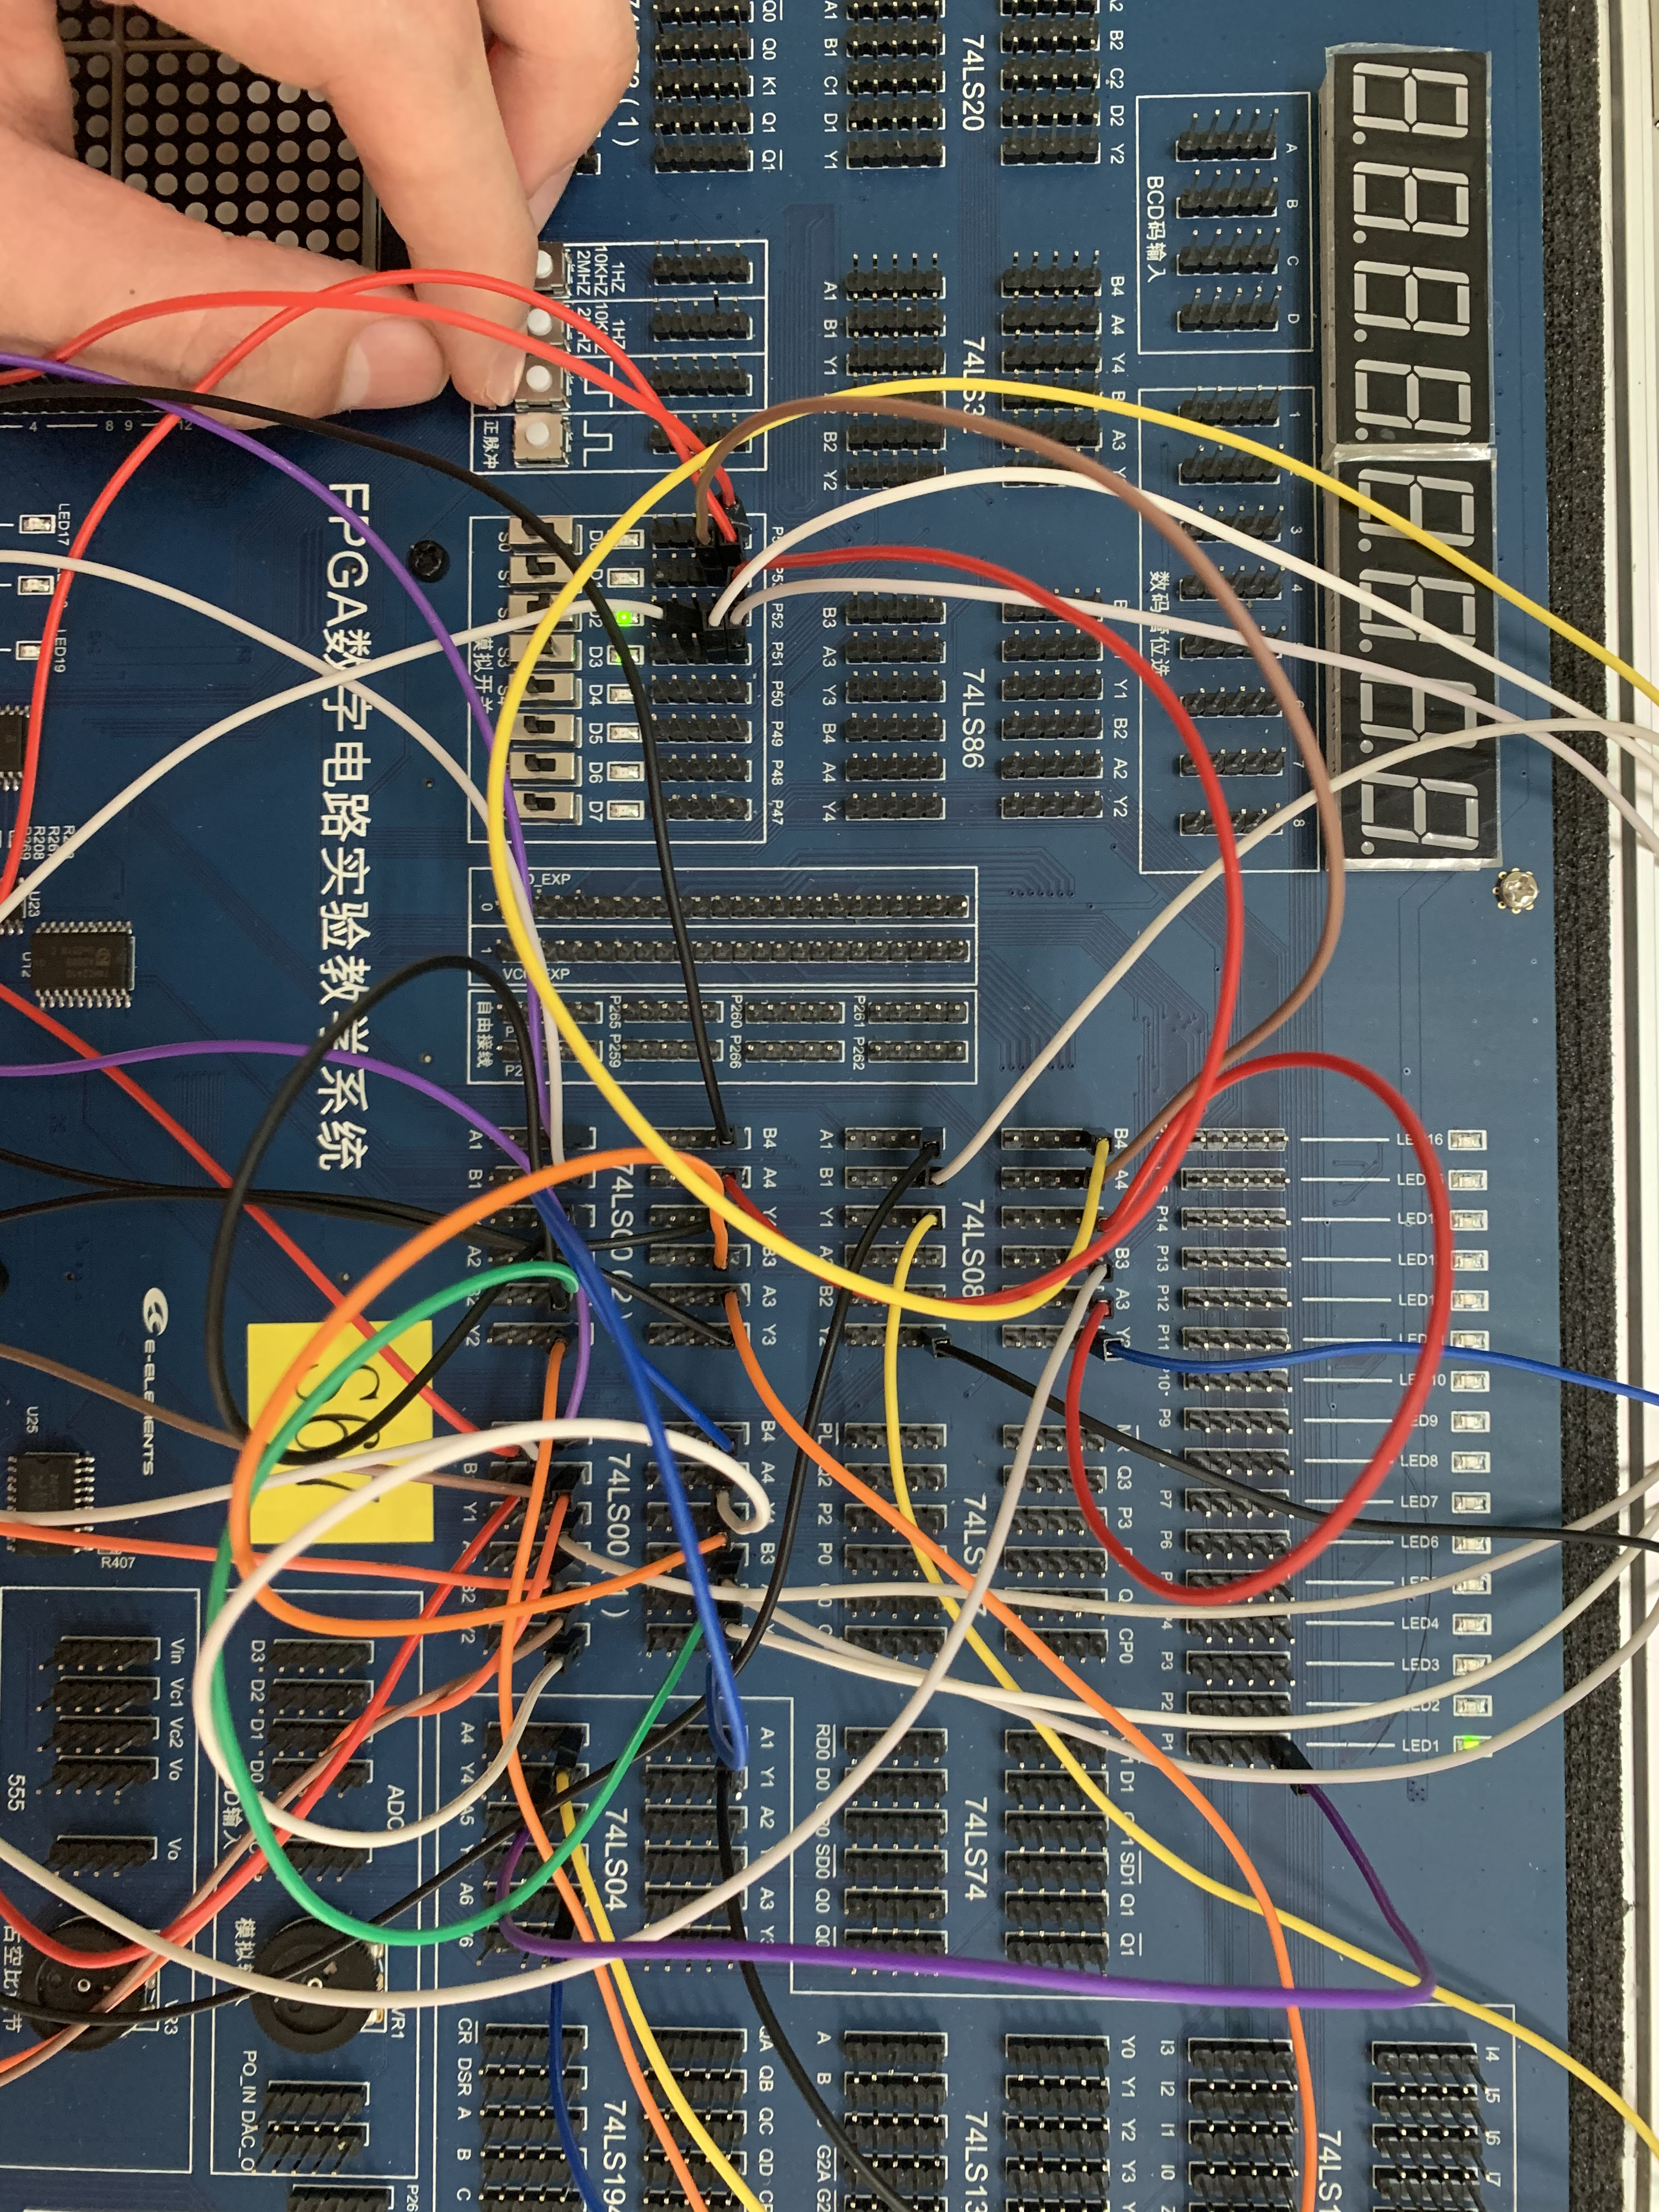
\includegraphics[width=0.8\textwidth]{1100.JPG}
\end{figure}
\begin{figure}[H]
    \centering
    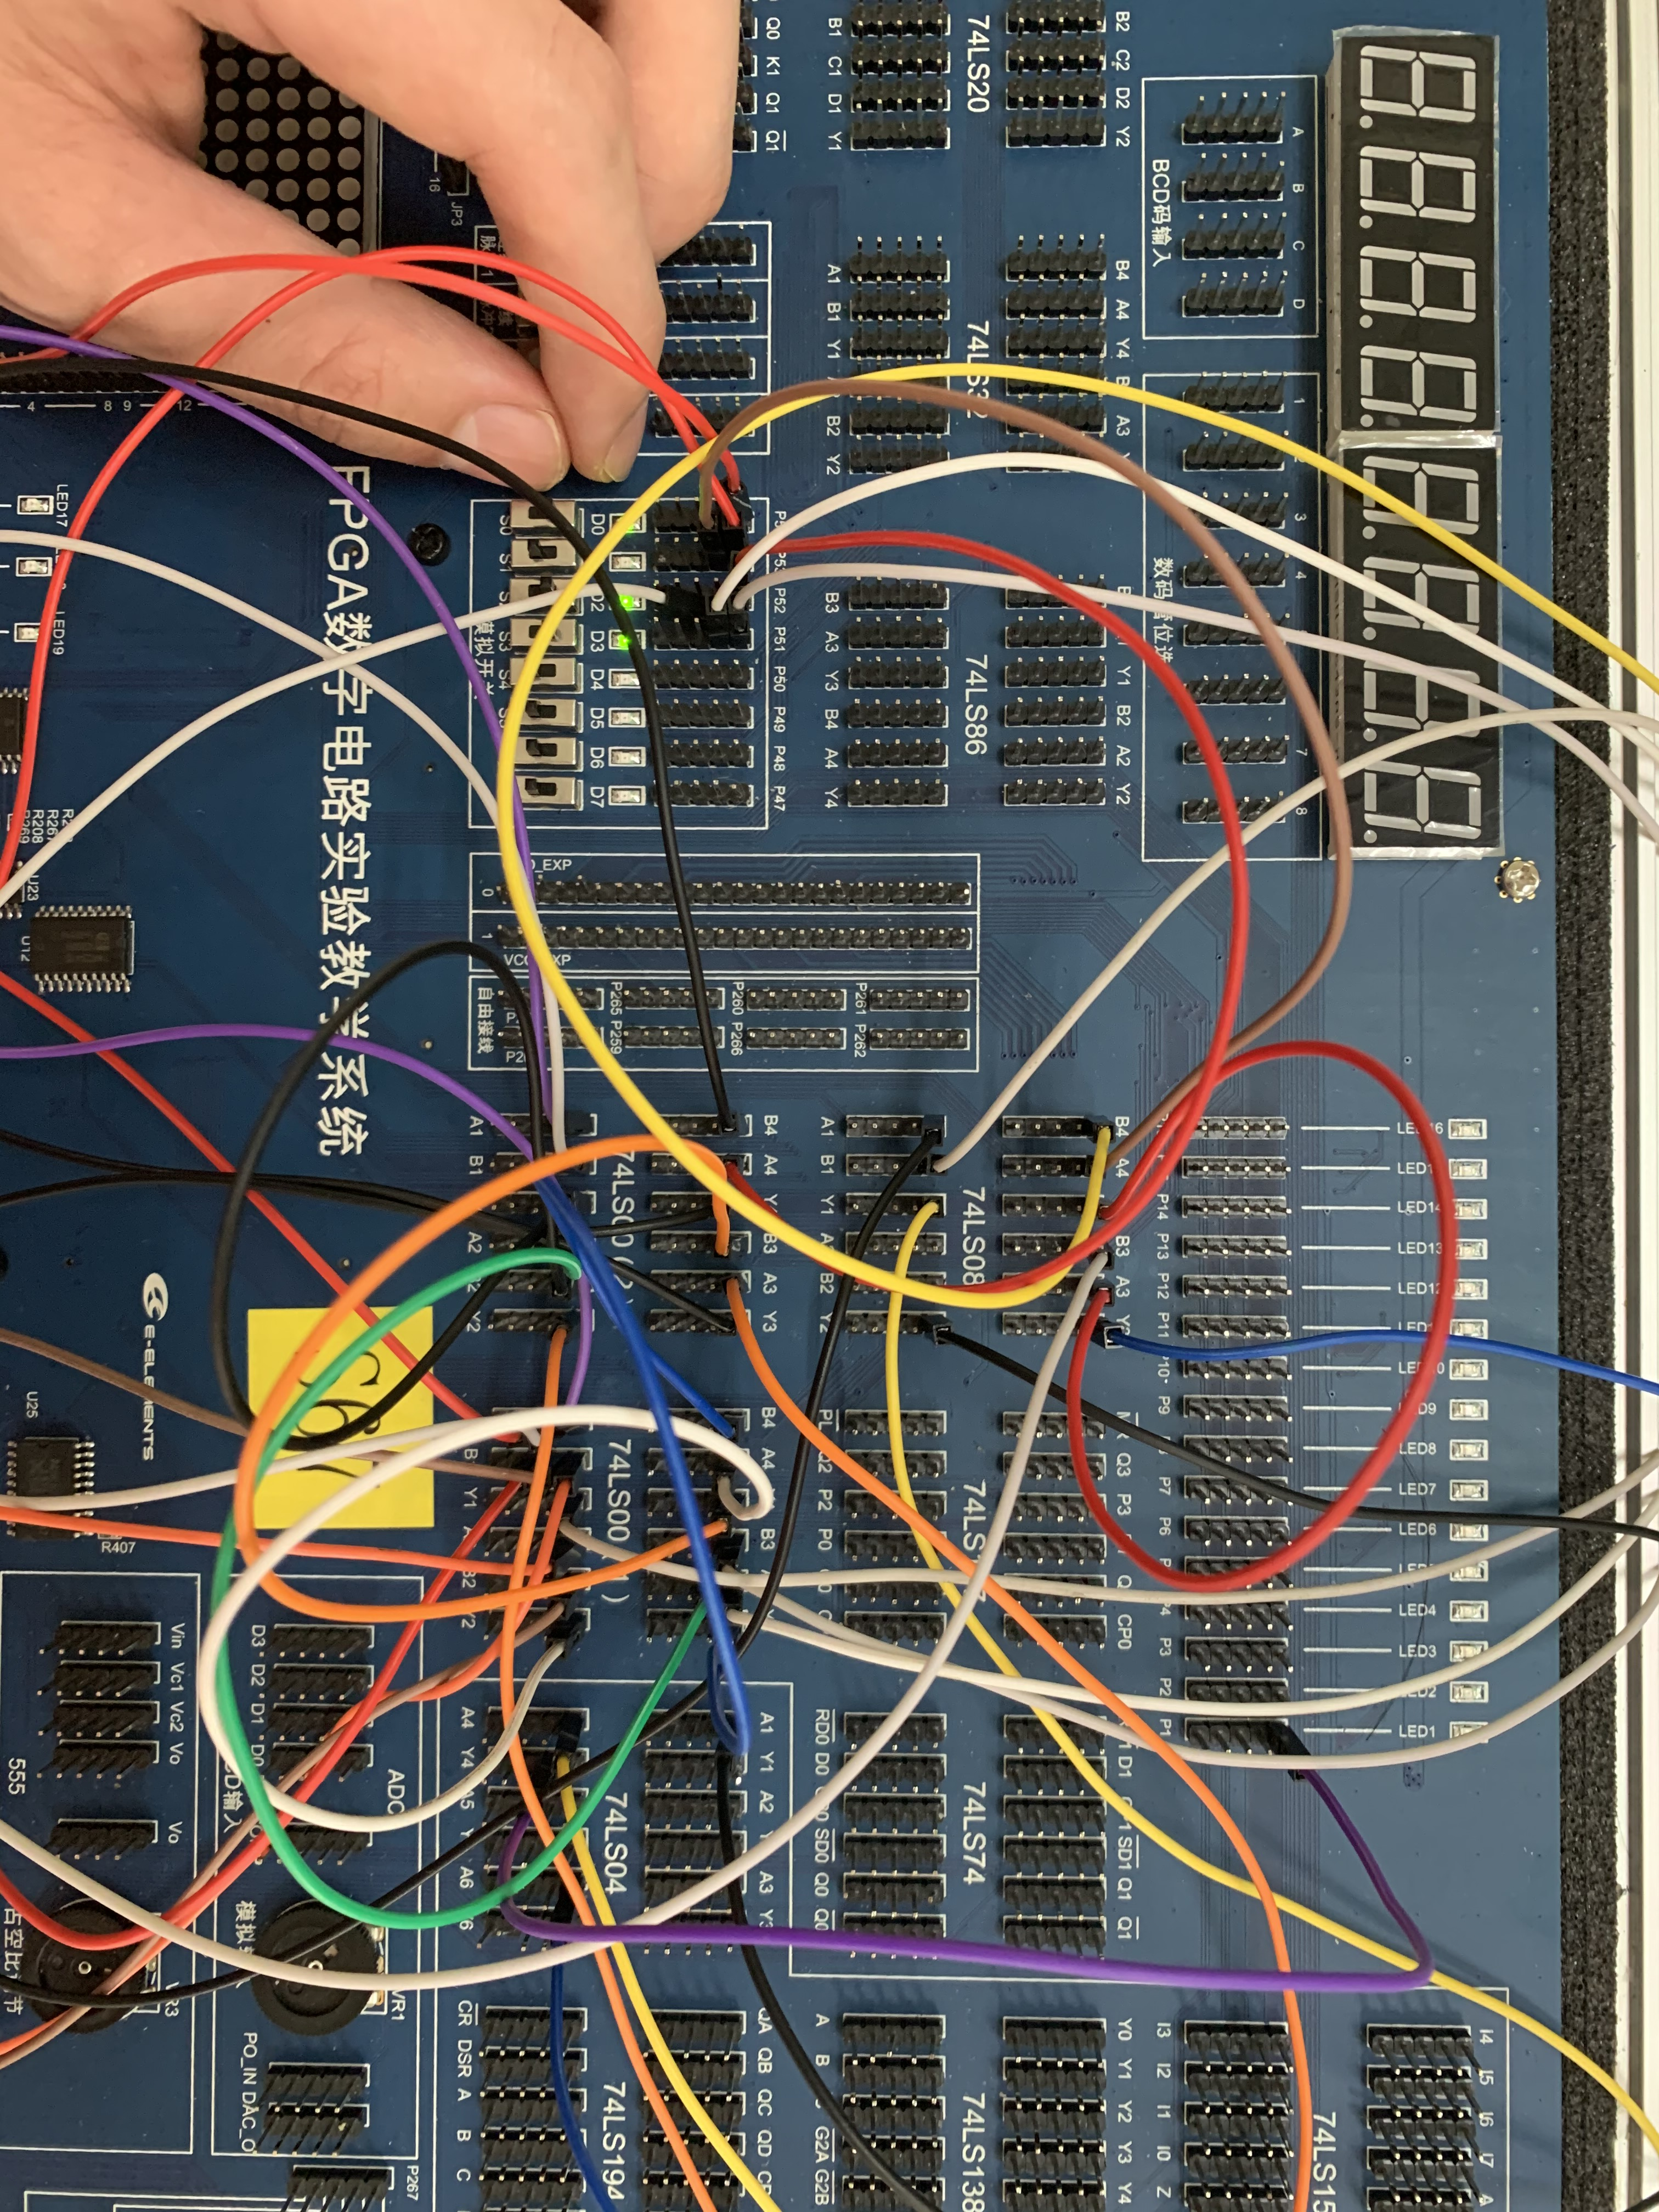
\includegraphics[width=0.8\textwidth]{1101.JPG}
\end{figure}
\begin{figure}[H]
    \centering
    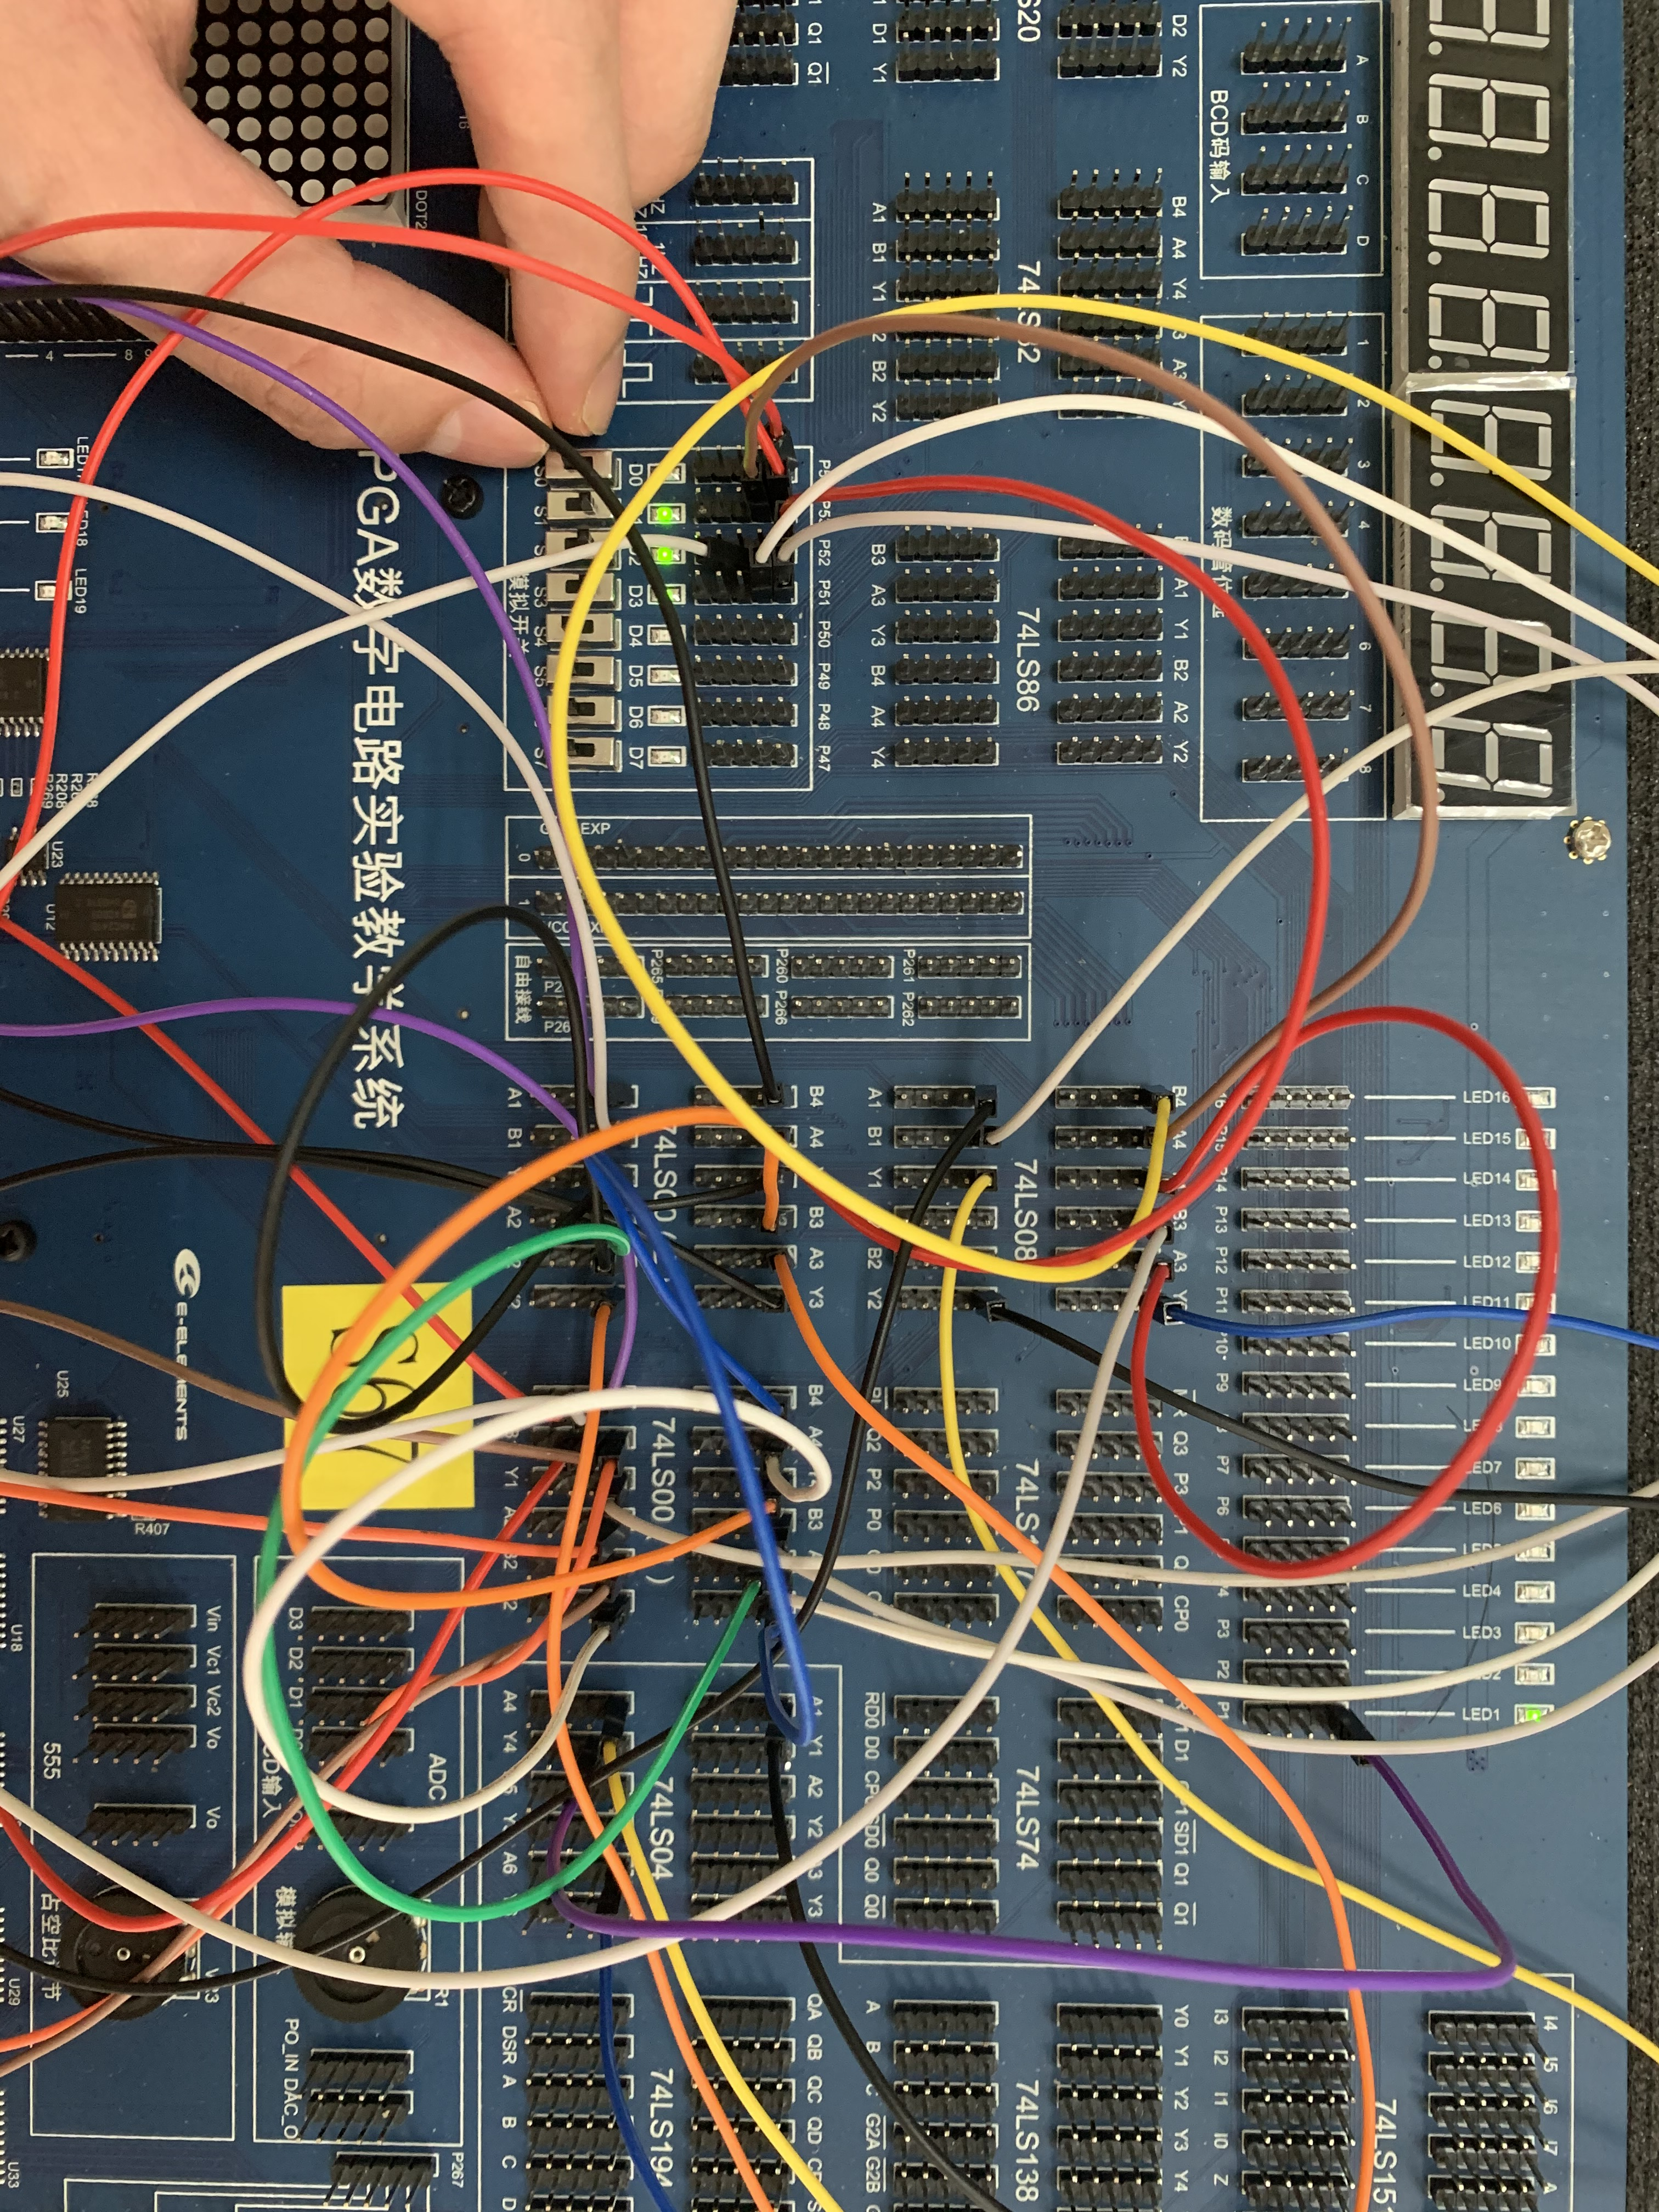
\includegraphics[width=0.8\textwidth]{1110.JPG}
\end{figure}
\begin{figure}[H]
    \centering
    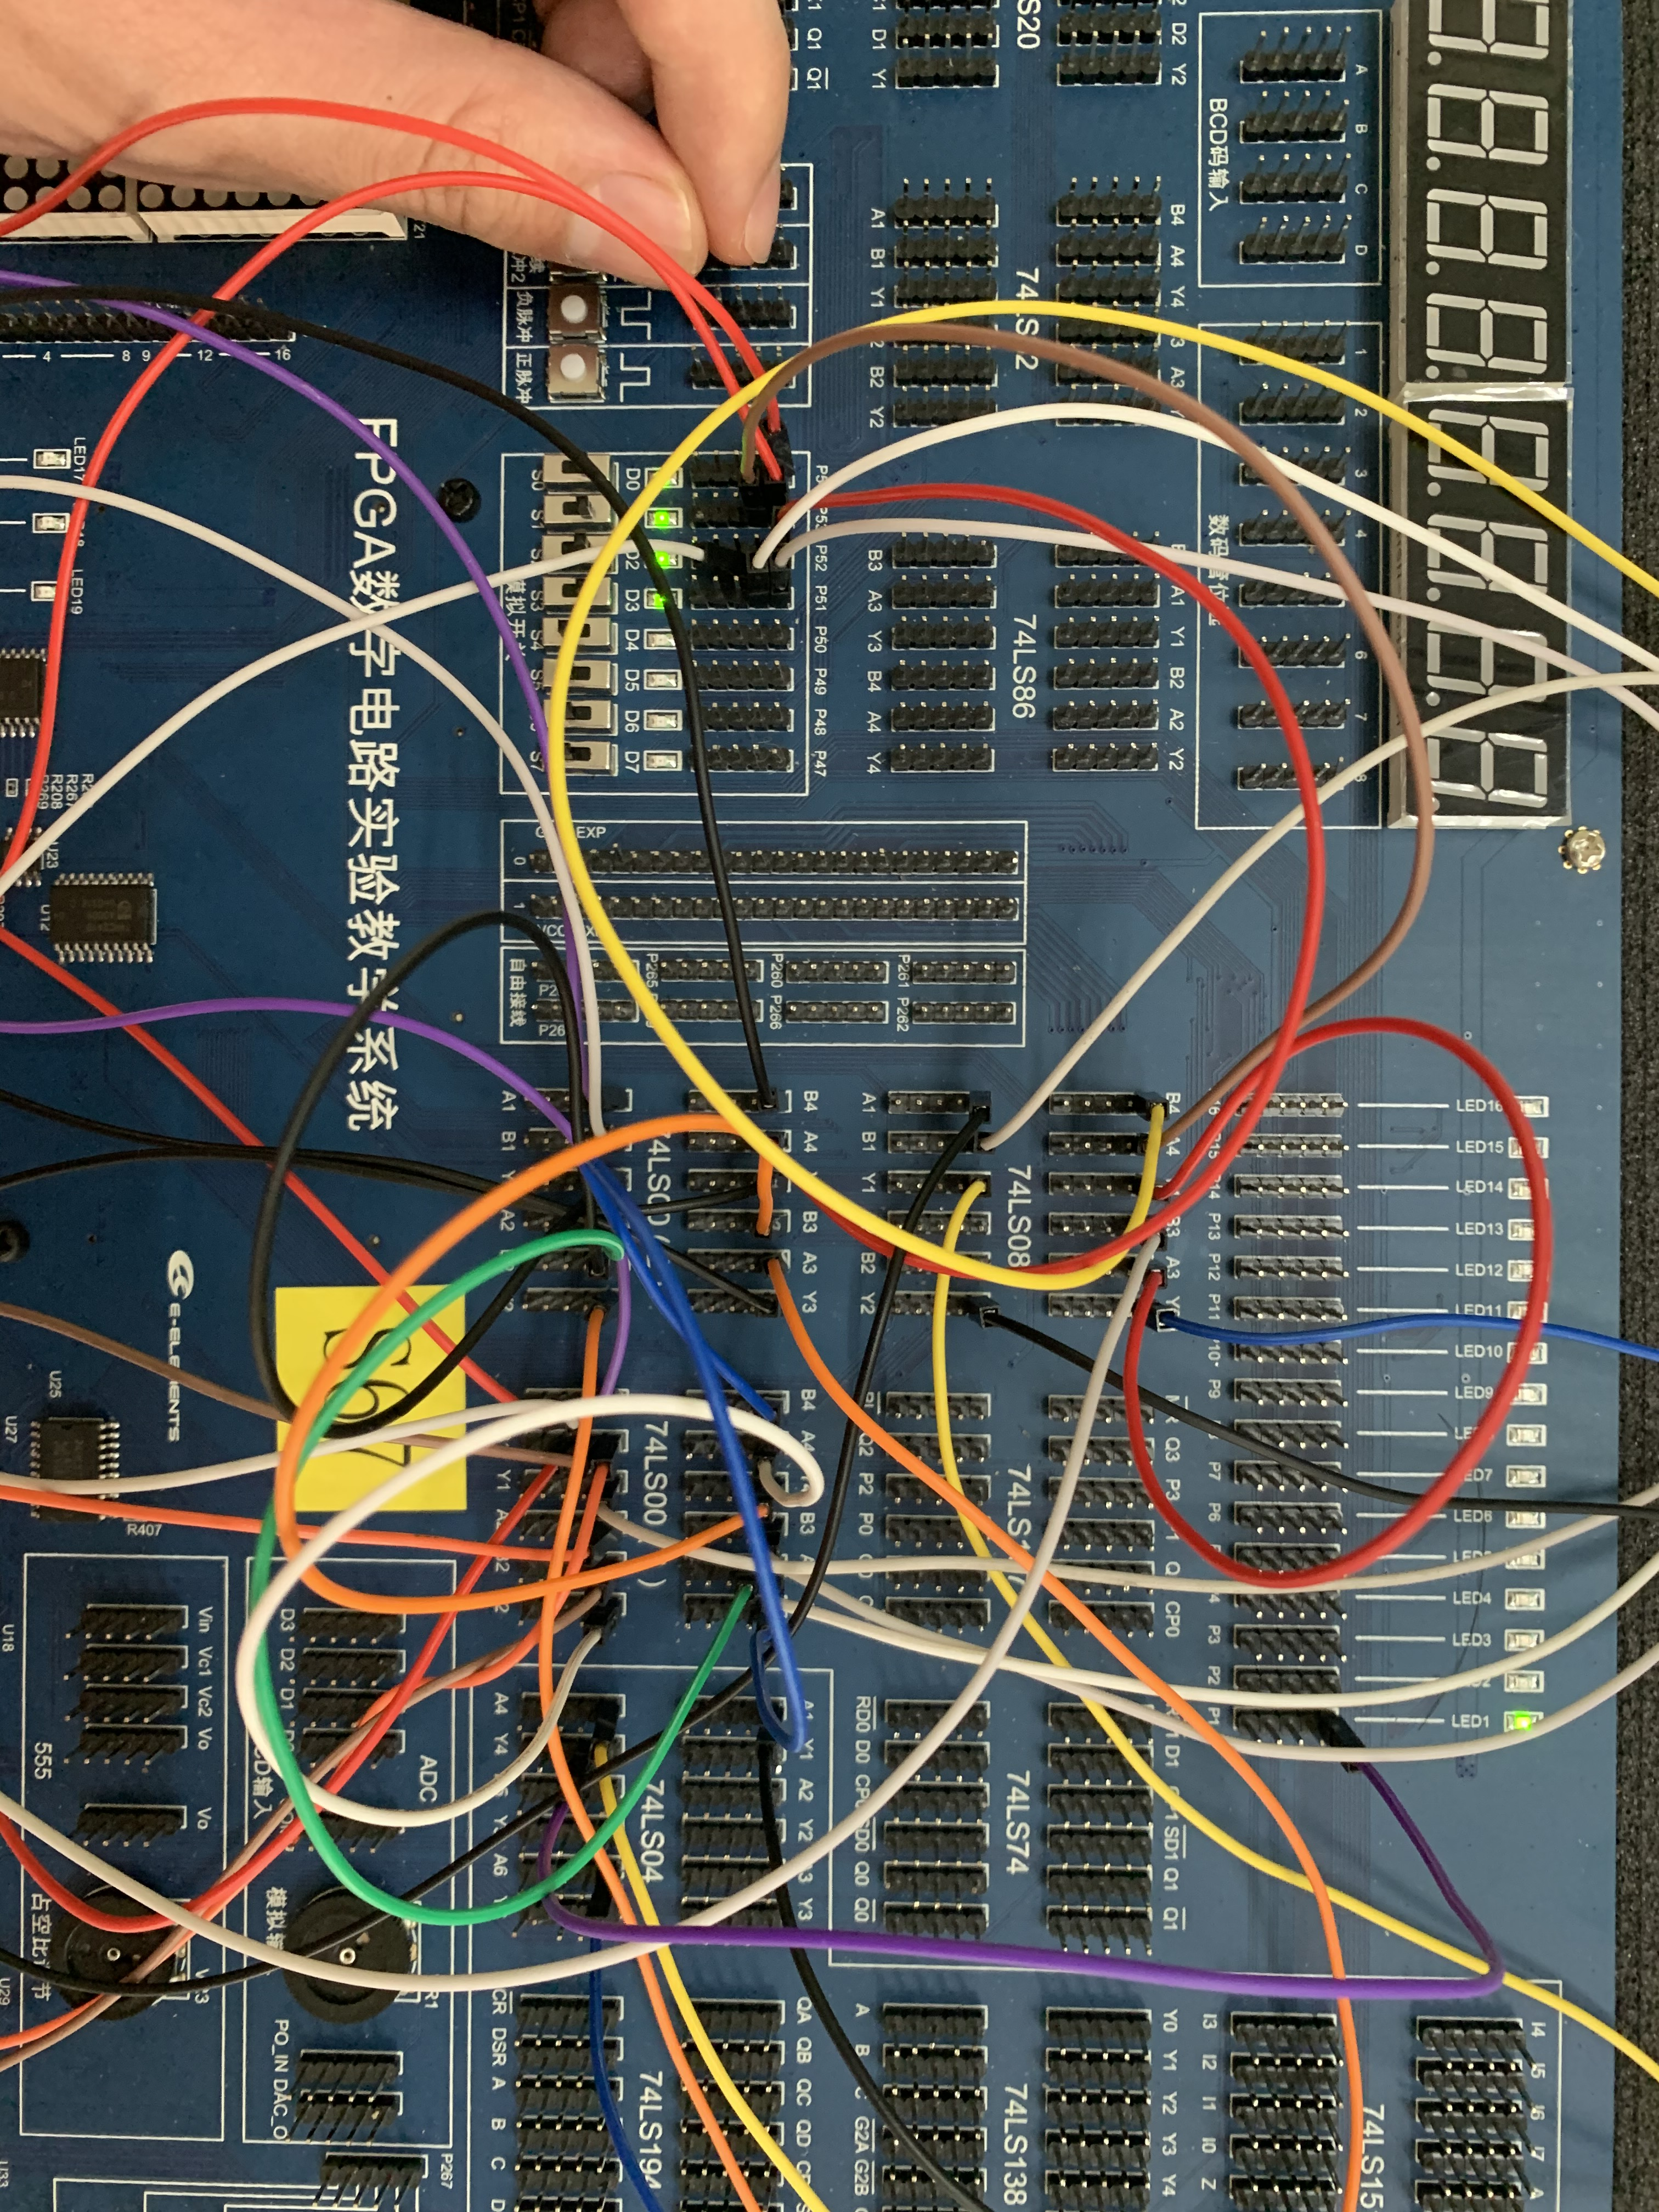
\includegraphics[width=0.8\textwidth]{1111.JPG}
\end{figure}
\subsubsection{五、2.(4)}
\begin{figure}[H]
    \centering
    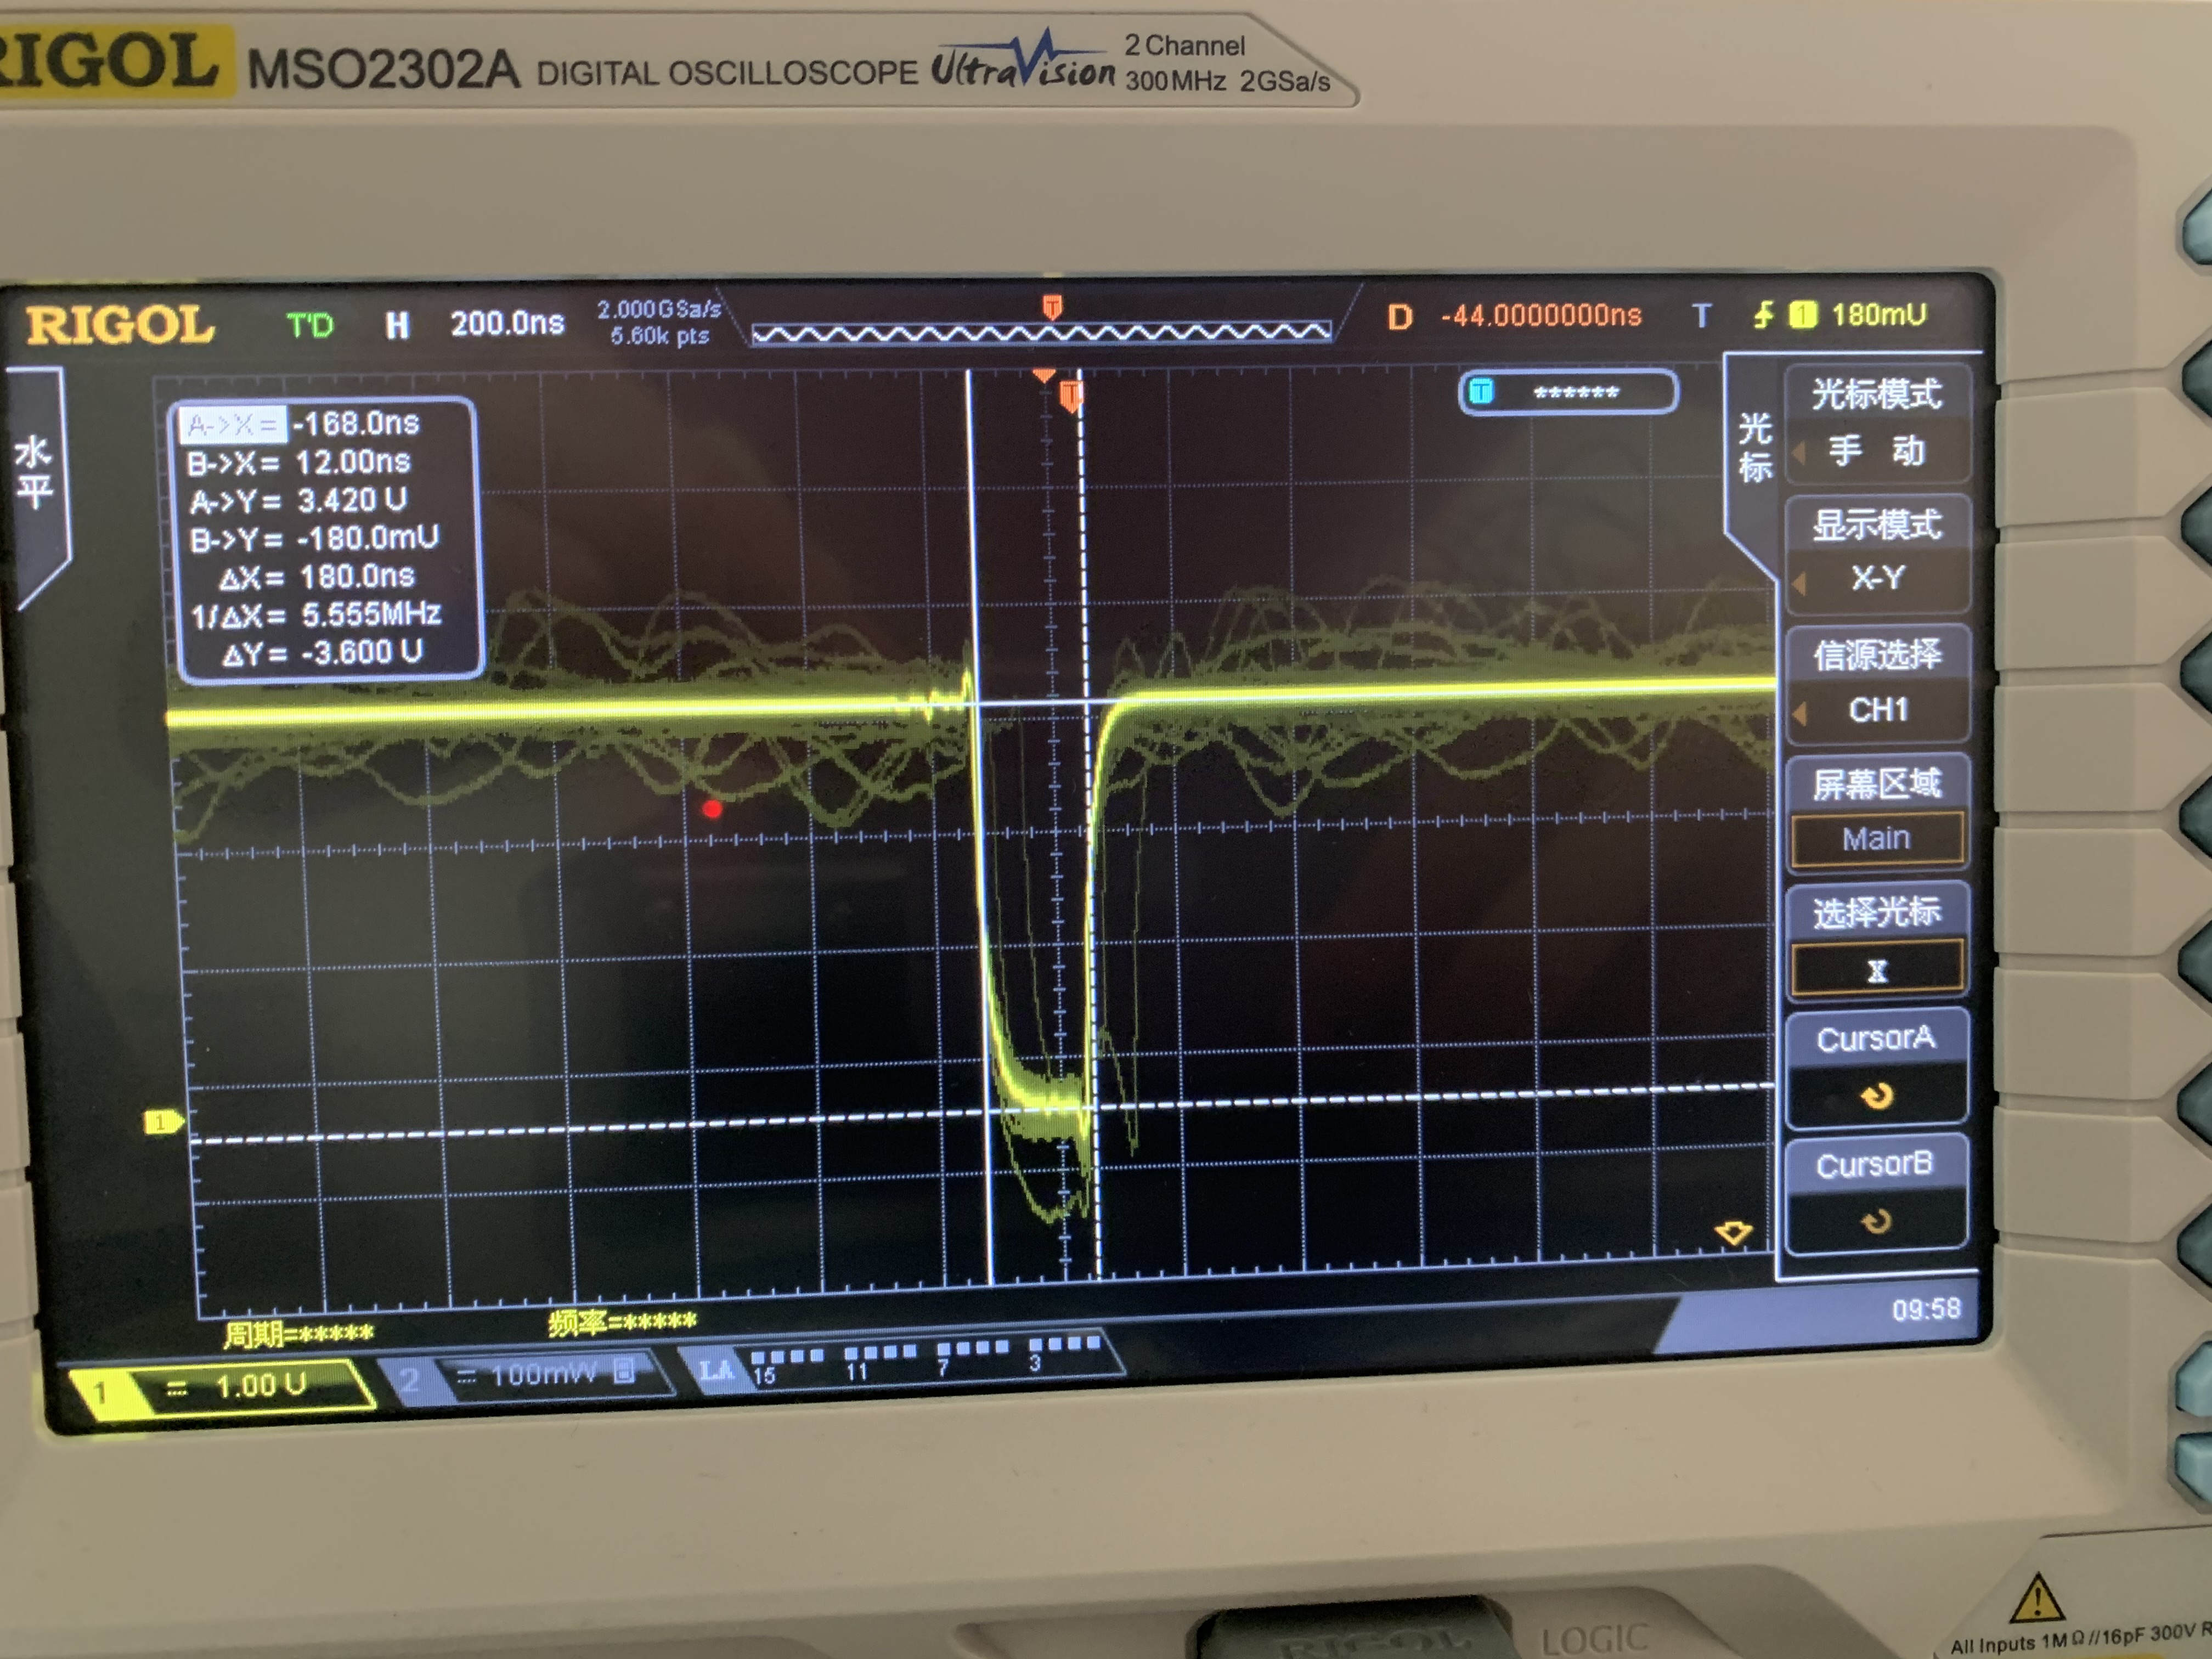
\includegraphics[width=0.8\textwidth]{模拟.JPG}
\end{figure}
$$V_{max}=3.6V$$
$$t_w=180ns$$
毛刺出现原因是$A$和$\bar A$输出均有延迟,当$A$变化时吗,两者难以同时改变输出。
\subsubsection{五、2.(5)}
\begin{figure}[H]
    \centering
    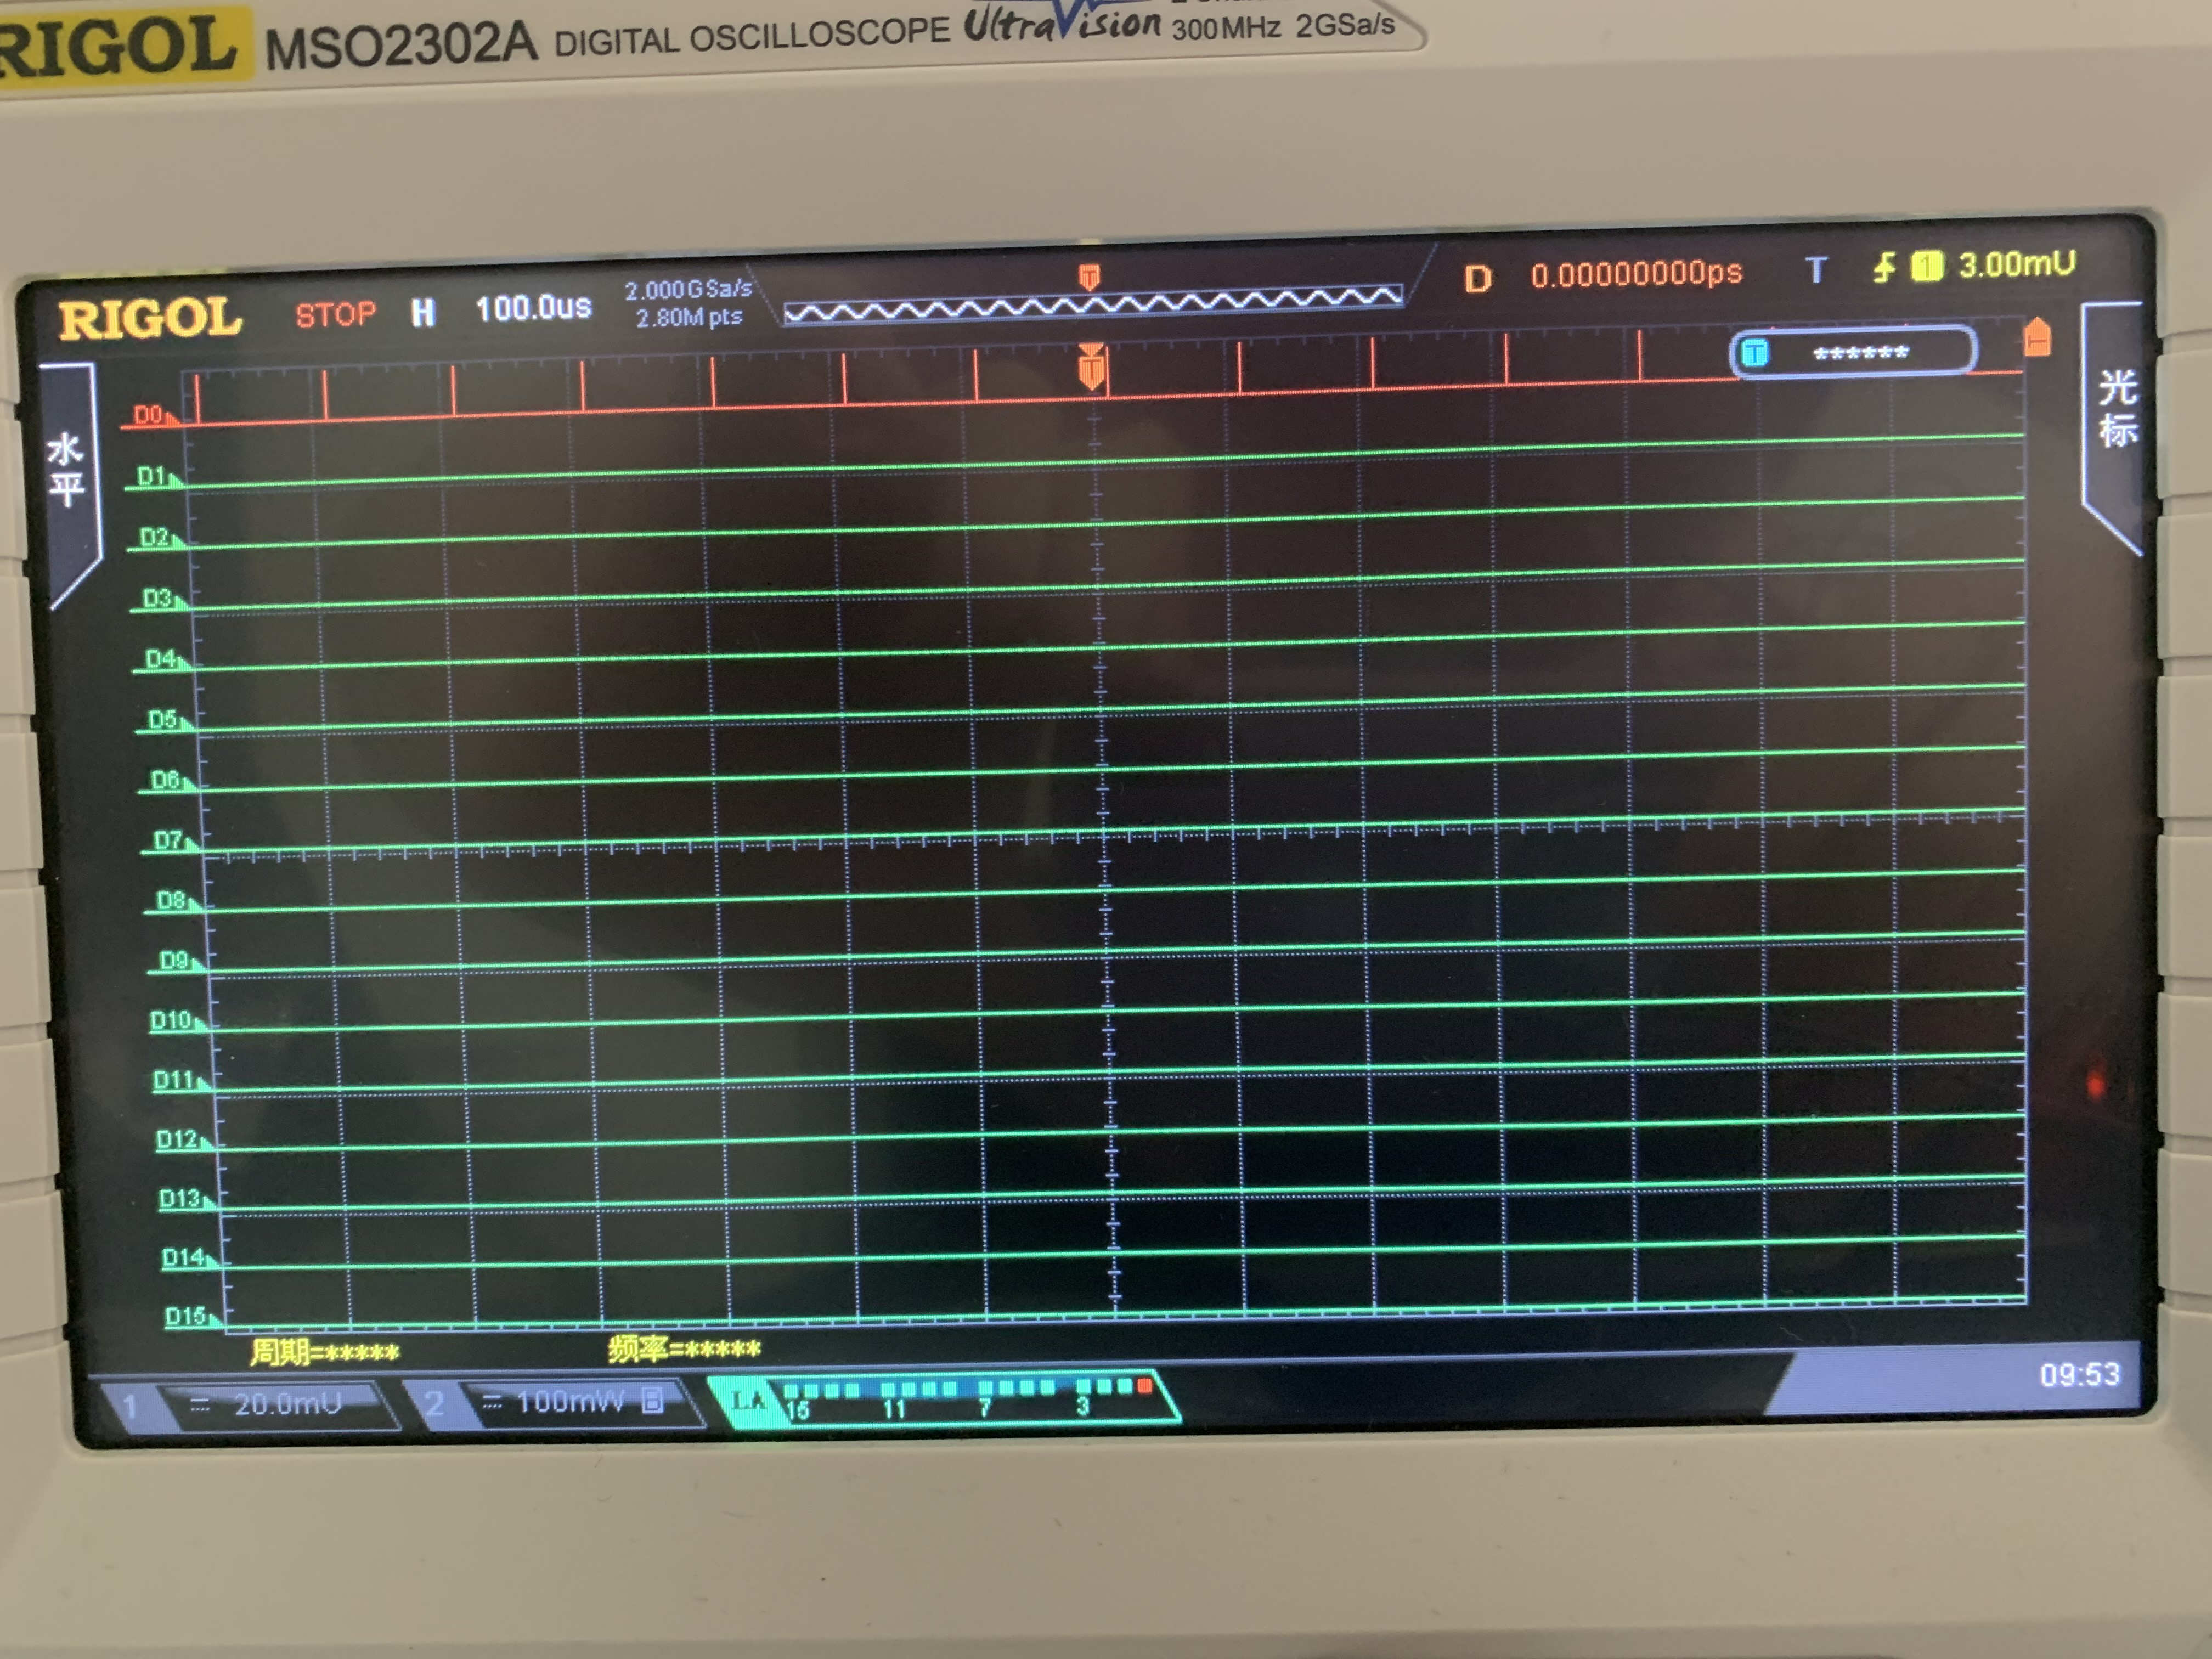
\includegraphics[width=0.8\textwidth]{反相.JPG}
\end{figure}
影响,因为毛刺也被输入到下一级电路中,相当于一个特殊的输入波形。
\subsection{思考题}
\begin{figure}[H]
    \centering
    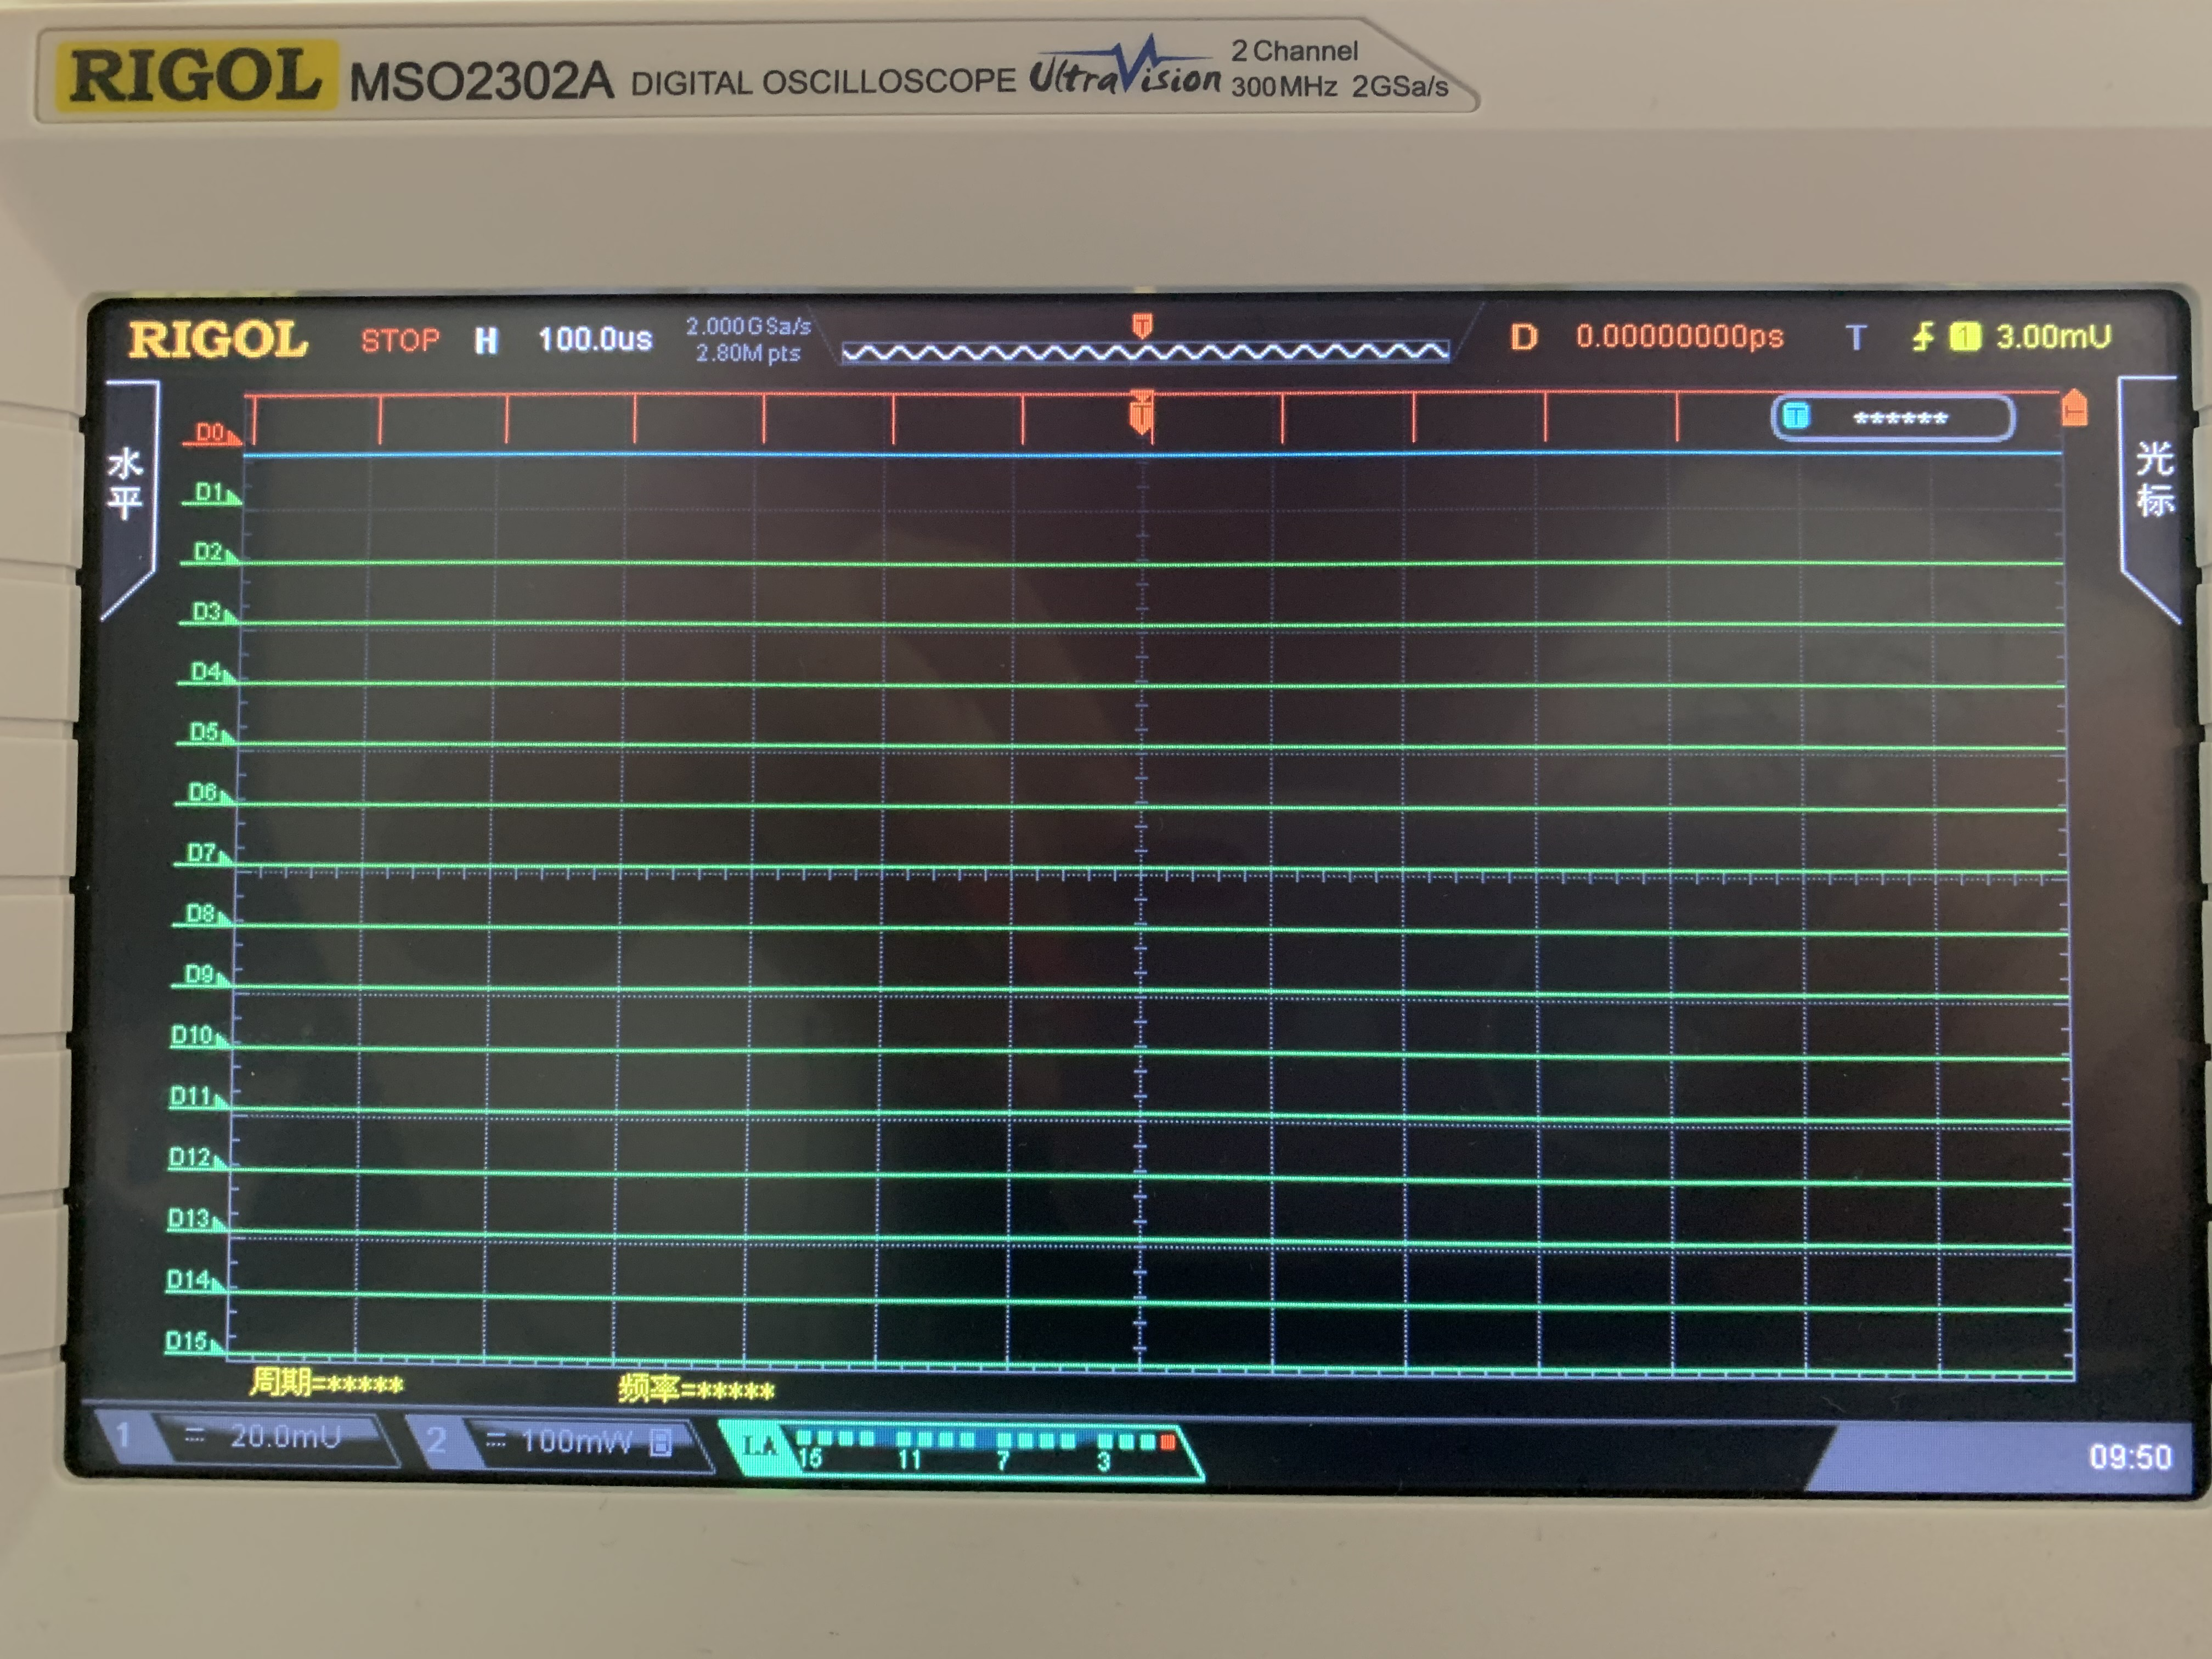
\includegraphics[width=0.8\textwidth]{冗余.JPG}
\end{figure}
D0是F,D1是F加冗余BCD,解决了毛刺。
\section{实验总结}
连接了更复杂的电路,了解了竞争冒险现象。
%\clearpage
%\bibliography{E:/Papers/LiuLab}
%\bibliographystyle{apalike}
\end{document}
%%% Local Variables:
%%% mode: latex
%%% TeX-master: t
%%% End:
